% Customizable fields and text areas start with % >> below.
% Lines starting with the comment character (%) are normally removed before release outside the collaboration, but not those comments ending lines

% svn info. These are modified by svn at checkout time.
% The last version of these macros found before the maketitle will be the one on the front page,
% so only the main file is tracked.
% Do not edit by hand!
\RCS$Revision: 401995 $
\RCS$HeadURL: svn+ssh://svn.cern.ch/reps/tdr2/notes/AN-16-378/trunk/AN-16-378.tex $
\RCS$Id: AN-16-378.tex 401995 2017-05-02 11:44:29Z stiegerb $
%%%%%%%%%%%%% local definitions %%%%%%%%%%%%%%%%%%%%%
% This allows for switching between one column and two column (cms@external) layouts
% The widths should  be modified for your particular figures. You'll need additional copies if you have more than one standard figure size.
\newlength\cmsFigWidth
\ifthenelse{\boolean{cms@external}}{\setlength\cmsFigWidth{0.85\columnwidth}}{\setlength\cmsFigWidth{0.4\textwidth}}
\ifthenelse{\boolean{cms@external}}{\providecommand{\cmsLeft}{top\xspace}}{\providecommand{\cmsLeft}{left\xspace}}
\ifthenelse{\boolean{cms@external}}{\providecommand{\cmsRight}{bottom\xspace}}{\providecommand{\cmsRight}{right\xspace}}
\newcommand{\tHq}{\ensuremath{\cPqt\PH\cPq}}
\newcommand{\tHW}{\ensuremath{\cPqt\PH\PW}}
\newcommand{\tH}{\ensuremath{\cPqt\PH}}
\newcommand{\ttH}{\ensuremath{\ttbar\PH}}
\newcommand{\ttZ}{\ensuremath{\ttbar\Z}}
\newcommand{\ttW}{\ensuremath{\ttbar\PW}}
\newcommand{\ttV}{\ensuremath{\ttbar\mathrm{V}}}
\newcommand{\WW}{\ensuremath{\PW\PW}\xspace}
\newcommand{\WZ}{\ensuremath{\PW\Z}\xspace}
\newcommand{\ZZ}{\ensuremath{\Z\Z}\xspace}
\newcommand{\tautau}{\ensuremath{\Pgt\Pgt}\xspace}
\newcommand{\Zll}{\ensuremath{\mathrm{Z}\to\ell^+\ell^-}\xspace}
\newcommand{\Ztt}{\ensuremath{\mathrm{Z}\to\tau^+\tau^-}\xspace}
\newcommand{\reliso}{\ensuremath{I_\mathrm{rel}}\xspace}
\newcommand{\sip}{\ensuremath{S_\mathrm{IP3D}}\xspace}
\newcommand{\Pgth}{\ensuremath{\Pgt_{\rm h}}\xspace}
\newcommand{\ptRatio}{\ensuremath{\pt^\text{ratio}}\xspace}
\newcommand{\ptRel}{\ensuremath{\pt^\text{rel}}\xspace}
\newcommand{\relIso}{\ensuremath{I_\text{rel}}\xspace}
\newcommand{\miniIso}{\ensuremath{I_\text{mini}}\xspace}
\newcommand{\CV}{\ensuremath{\kappa_\text{V}}\xspace}
\newcommand{\Ct}{\ensuremath{\kappa_\cPqt}\xspace}
\newcommand{\ft}{\ensuremath{f_\cPqt}\xspace}
\newcommand{\mumu}{\ensuremath{\Pgm^\pm\Pgm^\pm}\xspace}
\newcommand{\emu}{\ensuremath{\Pe^\pm\Pgm^\pm}\xspace}
\newcommand{\ee}{\ensuremath{\Pe^\pm\Pe^\pm}\xspace}
\newcommand{\threel}{\ensuremath{\ell\ell\ell}\xspace}
%%%%%%%%%%%%%%%  Title page %%%%%%%%%%%%%%%%%%%%%%%%
\cmsNoteHeader{AN-16-378} % This is over-written in the CMS environment: useful as preprint no. for export versions
% >> Title: please make sure that the non-TeX equivalent is in PDFTitle below
\title{Search for tHq production in \\ multilepton final states at 13~TeV}

% >> Authors
%Author is always "The CMS Collaboration" for PAS and papers, so author, etc, below will be ignored in those cases
%For multiple affiliations, create an address entry for the combination
%To mark authors as primary, use the \author* form
\address[unl]{University of Nebraska-Lincoln}
\address[tifr]{Tata Institute for Fundamental Research, Mumbai}
\author[unl]{Jose Monroy}
\author[tifr]{Pallabi Das}
\author[unl]{Benjamin Stieger}
\author[tifr]{Sandhya Jain}
\author[unl]{Ken Bloom}
\author[tifr]{Kajari Mazumdar}

% >> Date
% The date is in yyyy/mm/dd format. Today has been
% redefined to match, but if the date needs to be fixed, please write it in this fashion.
% For papers and PAS, \today is taken as the date the head file (this one) was last modified according to svn: see the RCS Id string above.
% For the final version it is best to "touch" the head file to make sure it has the latest date.
\date{\today}

% >> Abstract
% Abstract processing:
% 1. **DO NOT use \include or \input** to include the abstract: our abstract extractor will not search through other files than this one.
% 2. **DO NOT use %**                  to comment out sections of the abstract: the extractor will still grab those lines (and they won't be comments any longer!).
% 3. For PASs: **DO NOT use tex macros**         in the abstract: CDS MathJax processor used on the abstract doesn't understand them _and_ will only look within $$. The abstracts for papers are hand formatted so macros are okay.
\abstract{
   This note presents a search for the associated production of a Higgs boson with a single top quark in multilepton (same-sign dilepton or three leptons) final states, targeting Higgs decay modes to WW, ZZ, and $\tau\tau$. The full 2016 LHC dataset at 13 TeV is used. Limits are evaluated as a function of the Higgs couplings to vector bosons and top quarks.
}

% >> PDF Metadata
% Do not comment out the following hypersetup lines (metadata). They will disappear in NODRAFT mode and are needed by CDS.
% Also: make sure that the values of the metadata items are sensible and are in plain text:
% (1) no TeX! -- for \sqrt{s} use sqrt(s) -- this will show with extra quote marks in the draft version but is okay).
% (2) no %.
% (3) No curly braces {}.
\hypersetup{%
pdfauthor={Jose Monroy, Benjamin Stieger, Pallabi Das},%
pdftitle={Search for tHq production in multilepton final states at 13 TeV},%
pdfsubject={CMS},%
pdfkeywords={CMS, physics, higgs, top}}

\maketitle %maketitle comes after all the front information has been supplied
% >> Text
%%%%%%%%%%%%%%%%%%%%%%%%%%%%%%%%  Begin text %%%%%%%%%%%%%%%%%%%%%%%%%%%%%
%% **DO NOT REMOVE THE BIBLIOGRAPHY** which is located before the appendix.
%% You can take the text between here and the bibiliography as an example which you should replace with the actual text of your document.
%% If you include other TeX files, be sure to use "\input{filename}" rather than "\input filename".
%% The latter works for you, but our parser looks for the braces and will break when uploading the document.
%%%%%%%%%%%%%%%




\tableofcontents
\clearpage

\section{Introduction}
\label{sec:intro}
The Higgs boson discovery in 2012 by the CMS~\cite{HiggsCMS} and
ATLAS~\cite{HiggsAtlas} collaborations completed the picture of the
standard model
(SM) \cite{Salam:1961en,Glashow:1961tr,Weinberg:1967tq}
of the particle physics. Most of the basic properties of the Higgs
boson have been measured. However, several processes have very low
cross sections and it remains difficult to distinguish them from the
irreducible SM background processes with a similar signature. One of
the important but rare processes is a double Higgs (HH) boson
production that is sensitive to the Higgs boson self-coupling, therefore, 
has an access to the shape of the Higgs boson potential. In the SM HH
production is a non-resonant production with a cross section of $\sigma$
=  fb~\cite{HHXsec} at $\sqrt{s}=13$~TeV. Several Beyond the Standard
Model (BSM) theories and models, such as supersymmetry, composite Higgs, Warped Extra Dimensions (WED)~\cite{Dolan:2012ac, Huang:2017nnw, Kanemura:2016tan, Oliveira:2014kla, WED}, predict scenarios of the enhanced double Higgs boson
cross section.
There may be two cases: a non-resonant production,
introducing BSM terms to the SM lagrangian or a resonant production,
in which the process is mediated by a narrow width resonance
~\cite{WED}. %%\newline
\vspace{1em} % adds some space

In this analysis we examine the resonant di-Higgs production
through the gluon fusion mechanism mediated by a heavy narrow
resonance, such as RS1 KK graviton or RS1 radion ("graviton" or "radion" later in the text) \cite{BG1,BG2,BG3}. The analysis is performed for
masses of graviton/radion from 250 GeV to 1000 GeV. 95 \% upper confidence
limits are set on the production of the graviton with a subsequent
decay to Higgs bosons times the branching ratios of the Higgs
bosons decaying to a pair of b quarks and the other Higgs boson to two
leptons and two neutrinos respectively (Fig. ~\ref{fig:BGtoHH}). With the given data and
evaluated uncertainties, the results are compatible with the Standard
Model.


\begin{figure}[!htb]%hbpt?
  \begin{center}
    %\raisebox{0.17\height}
    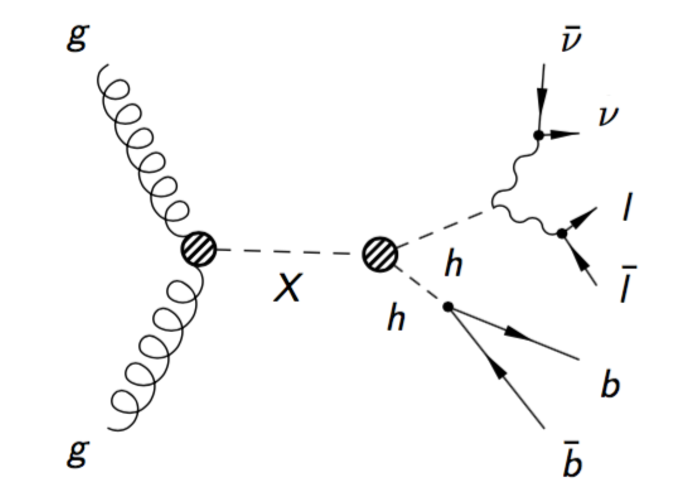
\includegraphics[width=0.45\textwidth]{figures/BGtoHH.pdf}
    \caption{ The Feynman diagram of the graviton production with the subsequent decay to a pair of the Higgs bosons. What follows is a decay to a pair of b quarks and Z bosons. Shown is 2 b quarks, 2 leptons, and 2 neutrinos final state.
    }
    \label{fig:BGtoHH}
  \end{center}
\end{figure}


\subsection{Analysis Strategy}

The analysis is based on ntuples and object selection from the approved VHbb sister analysis~\cite{VHbb_inspire}. Leptons, b jets, and the missing transverse energy (MET) are reconstructed using the standard CMS procedures~\cite{CMSreco} and the Particle Flow (PF) algorithm~\cite{PFalgo}. b-jets are identified using the Combined MVA v2 (CMVA) algorithm~\cite{BTagtwiki}. Then, on shell Z bosons are selected of dilepton pairs with a net charge zero for a pair. Higgs boson decaying to b quarks (Hbb) is reconstructed as a pair of b jets with the highest CMVA output value. Finally, double Higgs boson transverse mass, which is used in the shape analysis to extract limits, is constructed computing the transverse mass of the sum of the Lorentz vectors of the two leptons forming the on-shell Z, MET, and a pair of the b jets forming the \HBB. An additional cut on the missing transverse energy preserves the orthogonality with the existing HIG-18-013 ``2b 2l 2q'' analysis. Lastly, the cut on the BDT is used to reduce the background contamination in the signal region.

Main backgrounds are \ttbar and Drell-Yan in association with jets. Their normalization is extracted during the simultaneous fit of signal region (SR), as well as control region \ttbar (CRTT), and control region Drell-Yan (CRDY). Others, minor backgrounds, are single top production, diboson samples (WW, WZ, ZZ), and ZH production. 
%We assign systematics uncertainties on the QCD scale corresponding to each process. Also uncertainty associated with the imperfect knowledge of the single top cross section is added.

\clearpage

\section{Data and MC Samples}
\label{sec:samples}

%\subsection{Monte~Carlo samples\label{sec:mc}}

\subsection{Signal simulation\label{sec:signalMC}}

MC signal samples of the resonant Higgs boson pair production have been generated at the Leading Order (LO) using the \MADGRAPH~5 version\ ~2.2.2.0  generator ~\cite{Alwall:2014hca}. The gluon fusion production of a heavy narrow resonance is followed by the decay of the resonance into two SM Higgs bosons whose mass is fixed at 125~GeV.

Two signal MC samples are generated to cover the Higgs decay modes contributing to the 2 b jets 2 leptons 2 neutrinos final state of this measurement. The first sample type is a HH decay in to bbZZ channel, where one Higgs boson decays to a pair of b-quarks and the second Higgs boson decays into two Z bosons. In the second sample type bbVV events are generated, where HH can decay through bbWW and bbZZ channels. For both samples, the Z boson-pair and the W boson-pair are set to decay leptonically to two leptons and two neutrinos, where a lepton could be an electron or a muon. The second, bbVV, sample is filtered using the generator level information such that only the events with a W-boson pair (bbWW) are kept, while the Z-pair events are dropped: there are very few of them in the bbVV sample, and most importantly, high statistics bbZZ is taken from the dedicated bbZZ sample of the first type.

Events in the signal bbZZ and bbWW MC samples are normalised to 2~pb HH production cross section, which is a typical value of the heavy resonance production at 300 GeV predicted by the WED. Additionally the normalization includes the branching ratios of the Higgs boson decays contributing to the final state studied here: 0.0012 and 0.0266 for $HH\to bbZZ\to bb\ell\ell\nu\nu$ and $HH\to bbWW\to bb\ell\nu\ell\nu$, respectively \cite{CERNYR4}.

%%There are ten samples in the mass range of 260 to 1000 GeV generated for bbVV analysis and 16 samples for bbZZ from 250 GeV to 1000 GeV. Therefore, this document presents results for the masses where both signals are present. In the future we would consider doing approximations of the bbWW contribution where we have missing samples or generate them privately.

Unless mentioned otherwise, throughout the text plots and numbers represent the graviton study. The data and backgrounds for the radion measurement are the same, thus distributions also show the same good Data MC agreement and can be found for at Figs. ~\ref{fig:MCcomparisons} for the graviton case and ~\ref{fig:MCcomparisons_radion} for the radion case.

\subsection{Background simulation\label{sec:bkgMC}}

In this analysis the main backgrounds are \ttbar and Drell-Yan plus
jets with the mass of the boson greater than 50 GeV. Not all the
background processes pass our tight preselection (see section ~\ref{hhSelection}),
those which do, are single top, dibosons, and ZH backgrounds that are
listed in the Table \ref{tab:bg_mcsamples}:

\begin{table}[htbp]%H]
  %\footnotesize
  \begin{center}
    \caption{Background Monte Carlo samples\label{tab:bg_mcsamples}}
    \begin{tabular}{|c|}%|l|r|r|r|r|r|}
      \hline
      % Sample  & Generator & $m_{H} (\GeV/c^2)$ & $\sigma$ (pb) & events &  $\int\cal L$ (\fbinv) \\
      %\hline
      \multicolumn{5}{|l|}{\texttt{DY1JetsToLL\_M-50\_TuneCUETP8M1\_13TeV-madgraphMLM-pythia8}} \\
%                & \MADGRAPH\,5+\PYTHIA{}\,8 & 725 & 39 800 000 & 54.5 \\
      \multicolumn{5}{|l|}{\texttt{DY2JetsToLL\_M-50\_TuneCUETP8M1\_13TeV-madgraphMLM-pythia8}} \\
%               & \MADGRAPH\,5+\PYTHIA{}\,8 & 725 & 39 800 000 & 54.5 \\
      %\hline
      \multicolumn{5}{|l|}{\texttt{DY3JetsToLL\_M-50\_TuneCUETP8M1\_13TeV-madgraphMLM-pythia8}} \\
%              & \MADGRAPH\,5+\PYTHIA{}\,8 & 394.5 & 19 400 000  & 50.2 \\
      %\hline
      \multicolumn{5}{|l|}{\texttt{DY4JetsToLL\_M-50\_TuneCUETP8M1\_13TeV-madgraphMLM-pythia8}} \\
%             & \MADGRAPH\,5+\PYTHIA{}\,8 & 96.47 & 4 960 000 & 52.2 \\
      \multicolumn{5}{|l|}{\texttt{WW\_TuneCUETP8M1\_13TeV-pythia8}} \\
%            & \PYTHIA{}\,8 & 118.7 & 993 640 &  8.37  \\
      %\hline
      \multicolumn{5}{|l|}{\texttt{WZ\_TuneCUETP8M1\_13TeV-pythia8}} \\
%           & \PYTHIA{}\,8 & 47.13    &   1 000 000   &   21.22  \\
      %\hline
      \multicolumn{5}{|l|}{\texttt{ZZ\_TuneCUETP8M1\_13TeV-pythia8}} \\
%          & \PYTHIA{}\,8 & 16.523     &   985 600   &   59.65  \\
       \multicolumn{5}{|l|}{\texttt{ZH\_HToBB\_ZToLL\_M125\_13TeV\_aMC@NLO}} \\
      %\hline
      \multicolumn{5}{|l|}{\texttt{TT\_TuneCUETP8M1\_13TeV-powheg-pythia8}} \\
       %         & \POWHEG+\PYTHIA{}\,8 & 831.76   & 187 626 200 + 97 994 442&  343  \\
      %\hline
      \multicolumn{5}{|l|}{\texttt{ST\_tW\_top\_5f\_inclusiveDecays\_13TeV-powheg-pythia8\_TuneCUETP8M1}} \\
        %        & \POWHEG+\PYTHIA{}\,8 & 35.6   &   1 000 000   &   28.09  \\
      %\hline
      \multicolumn{5}{|l|}{\texttt{ST\_tW\_antitop\_5f\_inclusiveDecays\_13TeV-powheg-pythia8\_TuneCUETP8M1}} \\
         %       & \POWHEG+\PYTHIA{}\,8 & 35.6   &   999 400   &   28.07  \\
      %\hline\hline
      \multicolumn{5}{|l|}{\texttt{ST\_t-channel\_top\_4f\_leptonDecays\_13TeV-powheg-pythia8}} \\
          %      & \POWHEG+\PYTHIA{}\,8 & 136*0.325   &   999 400   &   22.6 \\
      %\hline
      \multicolumn{5}{|l|}{\texttt{ST\_t-channel\_antitop\_4f\_leptonDecays\_13TeV-powheg-pythia8}} \\
           %     & \POWHEG+\PYTHIA{}\,8 & 81*0.325   & 1 695 400 &  64.4 \\
      %\hline\hline
      \multicolumn{5}{|l|}{\texttt{ST\_s-channel\_4f\_leptonDecays\_13TeV-amcatnlo-pythia8}} \\
      %    & \POWHEG+\PYTHIA{}\,8 & 10.32   &   998 400   &   96.74  \\
\hline%\hline

    \end{tabular}
  \end{center}
  %\label{backgrounds} 
\end{table}



The simulated samples of the background processes such as 
~\ttbar~\cite{Frixione:2007nw} and the single top tW and t-channel
production processes~\cite{Frederix:2012dh} are generated at the
next-to-leading order (NLO) with POWHEG~\cite{Alioli:2009je}, while
single top s-channel production process is generated at NLO with
\MADGRAPH. \ttbar and single top production cross sections are
rescaled to the next-to-next-to-leading order (NNLO). 
Drell-Yan (DY)
process samples in association with 1, 2, 3 or 4 jets are generated
at the leading order using \MADGRAPH with the MLM
matching~\cite{Alwall:2007fs} and rescaled to NNLO using~\textsc{fewz}
program~\cite{Gavin:2010az,Li:2012wna,Gavin:2012sy}. 

As for the electroweak (EWK) order, DY samples have been rescaled to EWK NLO order with the NLO/LO k-factor of 1.23~\cite{DYkfactor}. Diboson samples
are generated at LO with {\PYTHIA}8.212~\cite{Sjostrand:2007gs}.

The main background
       process, which involves SM Higgs boson, is an associated
       production of the Higgs boson with a Z boson (ZH).  ZH process
       is simultated using the generator
%{{\sc MadGraph5_aMC@NLO}}                                                                                                                                                                               
$MadGraph5\_aMC@NLO$
~\cite{cite_aMC@NLO} with FxFx
merging~\cite{Frederix:2012ps} and
rescaled to NNLO with
{\MCFM} generator~\cite{Campbell:2010ff}.


For LO and NLO samples NNPDF3.0 parton distribution functions (PDF)
set is used. {\POWHEG} and {\MADGRAPH} interfaced with
{\PYTHIA}8.212~\cite{Sjostrand:2007gs} are used for the parton
showering and hadronization steps. To describe the underlying event
CUETP9M1 set derived in \cite{Khachatryan:2015pea} is
used. \GEANTfour~\cite{GEANT4} is used to model the response of the
CMS detector.

All the final cross sections denoted as NNLO are calculated at NNLO QCD accuracies and have been computed with the tool they were generated with. They found to be in agreement with the values from the LHC Higgs cross section working group ~\cite{LHCHXSWG, xsecZH, xsecTT, xsecST, xsecVV}.

During the data taking in 2016 the average number of proton-proton interactions per bunch crossing was 24 (denoted as pile up later), and in MC samples this information has been introduced overlapping these interactions with the events of interest.




\clearpage

\section{Object identification and event selection}
\label{sec:objects}
\subsection{Jets and \cPqb\ tagging}
The analysis uses anti-\kt\ (0.4) particle-flow (PF) jets, corrected for charged hadrons not coming from the primary vertex (charged hadron subtraction), and having jet energy corrections (\verb|Summer16_23Sep2016V3|) applied as a function of the jet $E_T$ and $\eta$.
Jets are only considered if they have a transverse energy above $25\GeV$.
% FIXME Something about forward jets?

In addition, they are required to be separated from any lepton candidates passing the fakeable object selections (see Tables~\ref{tab:muonIDs} and~\ref{tab:eleIDs}) by $\Delta\mathrm{R}>0.4$.

The loose and medium working points of the CSV \cPqb-tagging algorithm are used to identify \cPqb\ jets.
Data/simulation differences in the \cPqb\ tagging performance are corrected by applying per-jet weights to the simulation, dependent on the jet \pt, eta, \cPqb\ tagging discriminator, and flavor (from simulation truth)~\cite{btagRecommTWiki}.
The per-event weight is taken as the product of the per-jet weights, including those of the jets associated to the leptons.

More details can be found in the corresponding \ttH\ documentation~\cite{CMS_AN_2016-211,CMS_AN_2017-029}.

\subsection{Lepton selection}
The lepton reconstruction and selection is identical to that used in the \ttH\ multilepton analysis, as documented in Refs.~\cite{CMS_AN_2016-211,CMS_AN_2017-029}.
For details on the reconstruction algorithms, isolation, pileup mitigation, and a description of the lepton MVA discriminator and validation plots thereof, we refer to that document.

Three different selections are defined both for the electron and muon
object identification: the \emph{Loose}, \emph{Fakeable Object},
and \emph{Tight} selection.
As described in more detail later, these are used for event level vetoes, the fake rate estimation application region, and the final signal selection, respectively.
The \pt\ of fakeable objects is defined as $0.85\times\pt(\mathrm{jet})$, where the jet is the one associated to the lepton object.
This mitigates the dependence of the fake rate on the momentum of the fakeable object and thereby improves the precision of the method.

Tables~\ref{tab:muonIDs} and~\ref{tab:eleIDs} list the full criteria for the different selections of muons and electrons.

\begin{table}[h!]
\centering
\small
\topcaption{
\label{tab:muonIDs}
Requirements on each of the three muon selections. In the cases where
the cut values change between the selections, those values are listed in the table.
Otherwise, whether the cut is applied is indicated.
For the two \ptRatio\ and CSV rows, the cuts marked with a $\dagger$ are applied to leptons that fail the lepton MVA cut, while the loose cut value is applied to those that pass the lepton MVA cut.}
\begin{tabular}{cccc}
Cut & Loose & Fakeable object & Tight \\
\hline
$|\eta| < 2.4$         & \checkmark & \checkmark         & \checkmark \\
$\pt$                  & $>5\GeV$   & $>15\GeV$          & $>15\GeV$\\
$|d_{xy}| < 0.05$ (cm) & \checkmark & \checkmark         & \checkmark \\
$|d_z| < 0.1$ (cm)     & \checkmark & \checkmark         & \checkmark \\
$\text{SIP}_{3D} < 8$  & \checkmark & \checkmark         & \checkmark \\
\miniIso $< 0.4$       & \checkmark & \checkmark         & \checkmark \\
is Loose Muon          & \checkmark & \checkmark         & \checkmark \\
%\ptRatio              & --         & $>0.3\dagger$ / -- & -- \\
jet CSV                & --         & $< 0.8484$         & $ < 0.8484$ \\
%mva electron ID       & --         & $\ddagger$         & -- \\
is Medium Muon         & --         & --                 & \checkmark \\
tight-charge           & --         & --                 & \checkmark \\
lepMVA $> 0.90$        & --         & --                 & \checkmark \\
\hline
\end{tabular}
\end{table}


\begin{table}
\centering
\small
\topcaption{
\label{tab:eleIDs}
Criteria for each of the three electron selections. In cases where the cut values change between selections, those values are listed in the table. Otherwise, whether the cut is applied is indicated. In some cases, the cut values change for different $\eta$ ranges. These ranges are $0 < |\eta| < 0.8$, $0.8 < |\eta| < 1.479$, and $1.479 < |\eta| < 2.5$ and the respective cut values are given in the form (value$_1$, value$_2$, value$_3$).
}
\resizebox{1.0\linewidth}{!}{
\begin{tabular}{cccc}
Cut & Loose & Fakeable Object & Tight \\
\hline
$|\eta| < 2.5$                                  & \checkmark & \checkmark                   & \checkmark \\
$\pt$                                           & $>7\GeV$   & $>15\GeV$                    & $>15\GeV$      \\
$|d_{xy}| < 0.05$ (cm)                          & \checkmark & \checkmark                   & \checkmark \\
$|d_z| < 0.1$ (cm)                              & \checkmark & \checkmark                   & \checkmark \\
$\text{SIP}_{3D} < 8$                           & \checkmark & \checkmark                   & \checkmark \\
\miniIso $< 0.4$                                & \checkmark & \checkmark                   & \checkmark \\
MVA ID $> (0.0, 0.0, 0.7)$                      & \checkmark & \checkmark                   & \checkmark \\
$\sigma_{i\eta i\eta} <(0.011,0.011,0.030)$     & --         & \checkmark                   & \checkmark \\ %   & for corr. $\pt>30$ & for corr. $\pt>30$ \\
H/E $< (0.10,0.10,0.07)$                        & --         & \checkmark                   & \checkmark \\ %   & for corr. $\pt>30$ & for corr. $\pt>30$ \\
$\Delta\eta_{\textrm in} < (0.01, 0.01, 0.008)$ & --         & \checkmark                   & \checkmark \\ %   & for corr. $\pt>30$ & for corr. $\pt>30$ \\
$\Delta\phi_{\textrm in} < (0.04, 0.04, 0.07)$  & --         & \checkmark                   & \checkmark \\ %   & for corr. $\pt>30$ & for corr. $\pt>30$ \\
$-0.05 < 1/E-1/p < (0.010,0.010,0.005)$         & --         & \checkmark                   & \checkmark \\ %   & for corr. $\pt>30$ & for corr. $\pt>30$ \\
\ptRatio                                        & --         & $>0.5\dagger$ / --           & -- \\
jet CSV                                         & --         & $< 0.3 \dagger$ / $< 0.8484$ & $ < 0.8484$ \\
tight-charge                                    & --         & --                           & \checkmark \\
conversion rejection                            & --         & --                           & \checkmark \\
Number of missing hits                          & $<2$       & $== 0$                       & $== 0$ \\
lepMVA $> 0.90$                                 & --         & --                           & \checkmark \\
\hline
\end{tabular}}
\end{table}


\subsection{Lepton selection efficiency}
Efficiencies of reconstruction and selecting loose leptons are measured both for muons and electrons using a tag and probe method on both data and MC, using $Z\rightarrow\ell^{+}\ell^{-}$.
Corresponding scale factors are derived from the ratio of efficiencies and applied to the selected events.
These are produced for the leptonic SUSY analyses using equivalent lepton selections and recycled for the \ttH\ analysis as well as for this analysis.

The efficiencies of applying the tight selection as defined in Tables~\ref{tab:muonIDs} and~\ref{tab:eleIDs}, on the loose leptons are determined again by using a tag and probe method on a sample of DY-enriched events.
They are documented for the \ttH\ analysis in Ref.~\cite{CMS_AN_2017-029} and are exactly equivalent for this analysis.


%Two analysis methods are pursued to select samples that can be 
%used to extract the signal yield from the data in an optimal way.
\subsection{Higgs and Z Boson Selection}

Only dilepton pairs having net charge of zero are considered as \ZtoLL~ candidates. 
Pairs of prompt isolated leptons have to have a dilepton mass greater \
than 76 GeV. This ensures the orthogonality with HIG-17-006 bbVV analysis (later also referred to as bbWW analysis) as well as helps selecting decays of real Z bosons.

Higgs boson decays are reconstructed from the b jet pairs utilising only the two with the highest CMVAv2 discriminant value. We do not veto additional b jets. 

Double Higgs object is computed as a sum of Lorentz vectors of the \ZtoLL~ candidate, MET, and a \HBB~ candidate. Then, we compute the transverse mass of that object.

Transverse mass definition that we follow is one of the commonly used and is logical in the sense that we subtract the longitudinal momentum component which leaves us with the transverse momentum components only (while the energy remains the total energy).

More precisely, as the z-component of the neutrinos' momentum is unknown, we form a pseudo transverse mass:

%$M_T...with-tilda = $ (further referred as transverse mass for brevity), where E and pz are the energy and momentum of the candidate defined above.''                \
                                                                                                                                                                       

$\tilde{M}_T(HH) = \sqrt{E^2 - p_{z}^2}$ (further referred as transverse mass for brevity), where $E$ and \
$p_z$ are the energy and the Z-axis component of the Lorentz energy-momentum vector of the HH candidate.

The resulting distribution is what will be used in the binned shape analysis with the Higgs Combination Tool following the section ``Binned shape analysis'' as described at the twiki~\cite{CombinedLimit}.

%:
%\begin{center}
%    \small{\texttt{https://twiki.cern.ch/twiki/bin/view/CMS/SWGuideHiggsAnalysisCombinedLimit}}
%\end{center}

Analysis preselection to reduce ntuples size starts with the requirement on dilepton mass \toprule
 be greater than 50 GeV and the event to contain at least two jets with $p_{T} > 30$ GeV and $|\eta| < 2.4$. In addition to requirements on Higgs bosons decaying to b quarks mentioned above, we define Z bosons as two opposite sign muons with $p_{T} > 20/15$ GeV or two opposite sign electrons with $p_{T} > 25/15$ GeV. 



Later analysis cuts to improve signal-background separation include: the requirement on at least two b jets in the event, out of which two with the highest CMVAv2 score are used to define \HBB ~candidate. The lower end cut on the \HBB mass is set to 20 GeV to remove the low mass resonances while giving BDT as many events in the CRDY as possible at the same time. The upper end cut is not explicitly set for the same purpose. The actual \HBB mass distribution after the analysis selection is concentrated in the range 30 to 220 GeV. Then the Z boson selection cut takes the most energetic two leptons of the opposite sign and requires the their dilepton mass to pass 76 GeV < Z mass < 106 GeV selection used for the signal region definition. This is a standard +- 15 GeV window for Z boson selection whose lower end also preserves othogonality with the existing HIG-17-006 bbVV analysis. HH candidate is approximated by the sum of \ETslash, Z, and \HBB decays. A loose cut on HH transverse \textgreater~ 100 GeV removes evidently background events. Finally, an additional set of \ETslash cuts is used to ensure orthogonality with the existing HIG-18-013 bbZZ analysis focusing on the 2b jets + 2 leptons + 2 quarks, see Table \ref{metCuts}:


\begin{table}
\begin{center}
\caption{\ETslash cut to orthogonalise the analysis with respect to HIG-18-013.}
\begin{tabular}{|c|c|} \hline
{Signal mass, GeV} &  \ETslash cut, GeV\\\hline
260-300     &                                \textgreater~40 \\
350-600     &                                \textgreater~75 \\
650-1000    &                                \textgreater~100 \\
\hline
\end{tabular}
\label{metCuts}
\end{center}
\end{table}



\subsection{\HBB ~and \ZtoLL ~variables to define signal and control regions}

In this analysis we define three regions in the \HBB ~and \ZtoLL
~space. Two regions, CRDY and CRTT, are used to extract the
normalization of corresponding backgrounds. Signal region (Fig. ~\ref{fig:regions}) is chosen by
the set of \HBB~and \ZtoLL ~cuts \ref{fig:regions}. To reduce background contamination in this region, an additional cut on the MVA output is used. Boosted decision trees (BDT) MVA technique is employed to
separate background from signal. Below we describe in details
selection of each region and BDT construction. 

%% Skimming is applied
%% before building BDT to remove unnecessary background, while still
%% keeping a lot of events for BDT training. The set of "HH loose
%% common-sense" \label{hhSelection} skimming/preselection cuts includes: Dilepton (ee/mm)
%% mass $>$ 50 GeV, 2 or more jets: pt $>$ 30 GeV and $|\eta| < 2.4GeV$. Then, we
%% select two or more b-jets, \HBB~ mass should be greater than 20 GeV,
%% exactly two leptons, dilepton mass higher than 76 GeV, transverse mass
%% of HH higher than 100 GeV. The definition of the signal and control regions is illustrated in Fig. \ref{fig:regions}. The signal region is selected in the range of
%% 76 $<$ \mll~ $<$ 106 GeV and %75 $<$ \mbb~ $<$ 175 GeV. This corresponds to the
%% 90 $<$ \mbb~ $<$ 150 GeV. This corresponds to the
%% Z mass +- 15 GeV window. OA
For CRDY we invert \HBB ~cut, keeping in the lower sideband only events
with the mass of Higgs boson higher than 20 GeV to avoid fakes from
QCD. For CRTT we invert \ZtoLL ~cut, keeping only high mass sideband to
ensure the orthogonality with the existing HIG-17-006 bbVV analysis.


\begin{figure}[!htb]%hbpt?                                                                       
  \begin{center}
    %\raisebox{0.17\height}                                                                      
    \includegraphics[width=0.45\textwidthz{regions.png}
    \caption{ Signal region, control region \ttbar, and control region Drell-Yan in the phase space of \ZtoLL \ ~and ~\HBB ~masses.    }
    \label{fig:regions}
  \end{center}
\end{figure}


%% \begin{table}
%% \begin{center}
%% \caption{Efficiency of the BDT selection requirement. Dielectron channel. Left: 300 GeV signal mass hypothesis. Right: 900 GeV case.}
%% \begin{tabular}{|c|c|c|} \hline
%% {Process} &  Efficiency at 300 GeV, \% &  Efficiency at 900 GeV, \% \\\hline

%% signal (bbZZ) &                       85 &                       86 \\
%% signal (bbWW) &                       60 &                       82 \\
%% \ttbar        &                       28 &                       $\sim$ 0 \\
%% Drell-Yan     &                       64 &                       $\sim$ 0 \\
%% Single top    &                       33 &                        1 \\
%% ZH            &                       76 &                        4 \\
%% Dibosons      &                       76 &                        2 \\\hline

%% \end{tabular}
%% \label{EfficiencyBDT}
%% \end{center}
%% \end{table}


\begin{table}                                                                                                                                                                          
\begin{center}                                                                                                                                                                         
\caption{Efficiency of the BDT selection requirement. ee channel (top) and mm channel (bottom). }
\begin{tabular}{|c|c|c|}
\hline
sample & Efficiency at 300 GeV, [\%] &  Efficiency at 900 GeV, [\%] \\
\hline
signal (bbZZ) &                        89.2 &                        94.9 \\
signal (bbWW) &                        75.0 &                        88.4 \\
\ttbar        &                        28.8 &                         0.2 \\
Drell-Yan     &                        74.2 &                         1.2 \\
Single top    &                        33.1 &                         1.1 \\
ZH            &                        88.8 &                        10.7 \\
Dibosons      &                        90.0 &                         5.0 \\
\hline
\end{tabular}

\begin{tabular}{|c|c|c|}
\hline
sample &  Efficiency at 300 GeV, [\%] &  Efficiency at 900 GeV, [\%] \\
\hline
signal (bbZZ) &                        58.1 &                        91.1 \\
signal (bbWW) &                        25.9 &                        96.3 \\
\ttbar        &                        13.6 &                         0.2 \\
Drell-Yan     &                        39.0 &                         0.8 \\
Single top    &                        13.0 &                         0.2 \\
ZH            &                        56.0 &                         8.4 \\
Dibosons      &                        51.4 &                         6.2 \\
\hline
\end{tabular}
\label{EfficiencyBDT}                                                                                                                                                                  
\end{center}                                                                                                                                                                           
\end{table} 





\begin{figure}[tbp]
  \begin{center}
    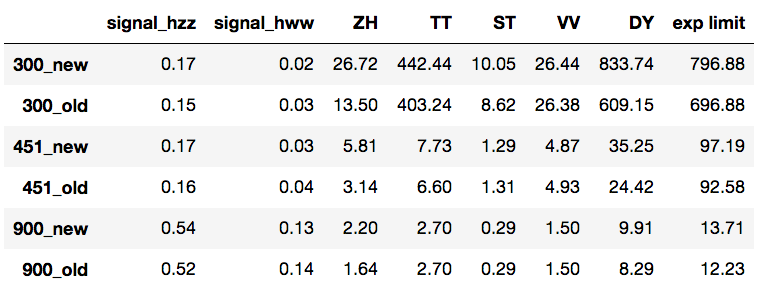
\includegraphics[width=0.91\textwidth]{ee_yields.png}
    \caption{Yields for ee channel before and after the tight isolation bug fix in the HEPPY. The effect is minimal as can be seen in the final limit. }
    \label{fig:yields_ee}
  \end{center}
\end{figure}



\subsection{Signal and background characteristics}

The signal region is further purified applying the cut in the BDT
output (Table ~\ref{EfficiencyBDT} contains the efficiency numbers for the BDT cut). 
The first set of BDT variables in the early version of the analysis included 30-50 variables, which could potentially discriminate signal from the background. The set containe\
d variables related to the kinematical properties of the signature, as well as a dozen of angular variables. After the first optimization, nine best variables were determined and chosen \
to be used for the analysis. Removal or addition of other variables did not improve the performance. %The same set of nine variables is used in both low and high mass trainings.


Following the procedure adopted by matured HH analyses, we
split the mass range into two: low mass and high mass (\`a la HIG-17-002 and HIG-17-008). These simplification costs some performance loss but allows analysis to proceed with just two BDTs instead of training one BDT per mass point, which would require more than a dozen of trainings per heavy resonance, though, training a dedicated BDT for each
signal mass hypothesis would give a better performance. However, the adopted path saves computational resources. Another reason is impracticality, bbZZ
signature is not the most sensitive, bb$\gamma$$\gamma$ is and the difference in sensitivity is a factor of 30-100 depending on the mass. More in the chapter \ref{sec:mva}.
%In addition, it would require a training of 16 BDTs per particle (BulkGraviton in our case). 
The low/high mass boundary value for HH analyses is chosen typically in the range 300-450
GeV. In our case the performance of the boundary around 300 GeV (area under the ROC curve
for low mass BDT is 0.9138 and 0.9805 for high mass BDT) is
similar to the boundary option at the 450 GeV (area under the ROC curve
for low mass BDT is 0.9086 and 0.9957 for high mass BDT), and to the one in the
middle of the range (area under the ROC curve
for 400 GeV for low mass BDT is 0.9074 and 0.9928 for high mass BDT). 
%https://indico.cern.ch/event/628835/contributions/2639777/attachments/1483653/2302207/Rami_HH_27June2017_v3.pdf
Therefore, we chose the value of 450 GeV, which
is also a choice of the bbbb analysis \cite{bbbb}. Upon running the full chain up to analysis limits, the choice of 450 GeV was confirmed to be the best split point option. As a result, the low
mass BDT includes a mix (with the weight '1') of seven signal samples:
250, 260, 270, 300, 350 400, 450 GeV. The high mass training includes nine
masses: 500, 550, 600, 650, 700, 750, 800, 900, 1000. In each case the
composition of the background is the same, it is a mix (by cross
section) of \ttbar and Drell-Yan plus jets.


Cut flow for ee and mm channels from the gen level up to before the BDT selection is shown on the figures ~\ref{fig:cutFlow}. In the cut flow table ~\ref{fig:cutFlow} the following definitions are used: very loose selection means all GsfElectrons and Muons from the basic collections that match gen-level electrons/muons and pass the very minimal kinematic cuts; loose selection means loose POG selection consisting of kinematic, dxy/dz, iso cuts. The final efficiency values represent these numbers in terms of events ~\ref{cutFlowEvents}:

\begin{table}
\begin{center}
\caption{Number of events surviving analysis cuts corresponding to the last entry in the ~\ref{fig:cutFlow} .}
\begin{tabular}{|c|c|c|} \hline
{Process, mass point} &  ee channel, \% &  mm channel, \% \\\hline
bbZZ, 300 GeV &                    2256     &                    4511 \\
bbWW, 300 GeV &                    53       &                    85 \\
bbZZ, 900 GeV &                    8034     &                    12963 \\
bbWW, 900 GeV &                    12       &                    23 \\\hline
\end{tabular}
\label{cutFlowEvents}
\end{center}
\end{table}






\subsubsection{Data and MC comparison\label{sec:compareDataMC}}
Signal region BDT side-band plots as well as unblind signal region plots show good data-MC agreements.
We are not cutting on BDT for control regions, therefore, all the mass
point have the same background and data distributions. 
That is
why we provide below plots for two mass points: one mass point representing low mass region, 300 GeV, and one mass point representing high mass region, 900 geV. 
% for other pass point only signal distribution will change,
%however, data/background comparison and their ratio will not. At the same time, BDT outputs are mass point specific, because are trained for two different mass regions - low and high mass regions, and are evaluated for each mass point separately. Thus, we show all the BDT plots. 
Signal bbZZ and bbWW rates for all plots are multiplied by some high factors depending on the mass point purely for the visualization purpose and do not go in the real analysis. 

Prefit plots are available in the Appendix ~\ref{sec:datamc}. Control regions only postfit plots have been produced during an extensive discussion with Higgs conveners at HyperNews, and it was shows that upon inclusion of the SR in the fit the data-MC agreement is slightly better. Postfit plots that include SR in simultaneous fit, hence a common jargon name ``Full postfit`` plots, are presented at the figures ~\ref{fig:MCcomparison_mm_300} - ~\ref{fig:MCcomparison_ee_900} and show data and MC comparison in the SR, CRDY, and CRTT. For both ee and mm channels, low and high mass regions. The latest style plots produced for the PAS can be found at Fig.~\ref{fig:MCcomparisons} for the graviton case and Fig.~\ref{fig:MCcomparisons_radion} for the radion case. 



Distributions of nine variables that go into the BDT have been studied in depth during the pre-approval process and are available in the Appendix ~\ref{sec:datamc}. After the tight isolation cut fix in the HEPPY framework the results/shapes are almost unchanged (it is also can be observed from the table of yields ~\ref{fig:yields_ee}).  At the yields table ~\ref{fig:yields_ee}, 450 GeV mass point, since evaluated using the high mass BDT, is called 451 GeV for clarity purposes. 



\begin{figure}[tbp]
  \begin{center}
    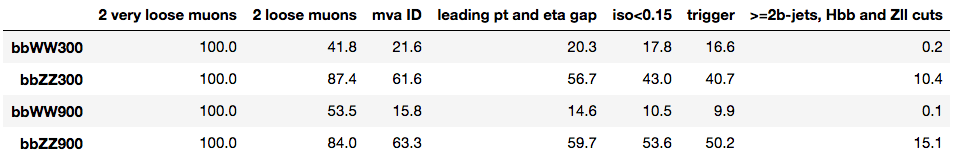
\includegraphics[width=0.91\textwidth]{cutflow_mm.png}\\
    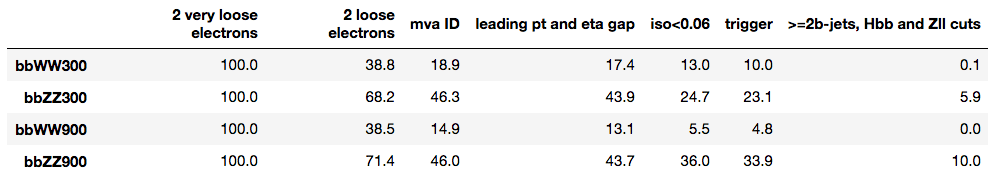
\includegraphics[width=0.91\textwidth]{cutflow_ee.png}\\
    \caption{Cut flow for mm (top) and ee (bottom) channels. }
    \label{fig:cutFlow}
  \end{center}
\end{figure}



%% \begin{figure}[tbp]                                                                                                                                           
%%   \begin{center}                                                                                                                                              
%%     \includegraphics[width=0.31\textwidth]{mm_300_july20/hhMt_mm_SR_FullPostfit_plot_july20.png}                                                  
%%     \includegraphics[width=0.31\textwidth]{mm_300_july20/hhMt_mm_CRDY_FullPostfit_plot_july20.png}
%%     \includegraphics[width=0.31\textwidth]{mm_300_july20/hhMt_mm_CRTT_FullPostfit_plot_july20.png}\\                                              
%%     \includegraphics[width=0.31\textwidth]{mm_300_july20/bdt_response_mm_SR_FullPostfit_plot_july20.png}                                         
%%     \includegraphics[width=0.31\textwidth]{mm_300_july20/bdt_response_mm_CRDY_FullPostfit_plot_july20.png}                                           
%%     \includegraphics[width=0.31\textwidth]{mm_300_july20/bdt_response_mm_CRTT_FullPostfit_plot_july20.png}\\                                
%%     \caption{Comparison of data and MC samples. 300 GeV, mm channel, Full Postfit plots. Top: hhMt, bottom: BDT distributions. From left to right: SR, CRDY, CRTT.}
%%     \label{fig:MCcomparison_mm_300}                                                                                                                   
%%   \end{center}                                                                                                                                                
%% \end{figure}                                                                                                                                                  


%% \begin{figure}[tbp]                                                                                                                                           
%%   \begin{center}                                                                                                                                              
%%     \includegraphics[width=0.31\textwidth]{ee_300_july20/hhMt_ee_SR_FullPostfit_plot_july20.png}                                                  
%%     \includegraphics[width=0.31\textwidth]{ee_300_july20/hhMt_ee_CRDY_FullPostfit_plot_july20.png}
%%     \includegraphics[width=0.31\textwidth]{ee_300_july20/hhMt_ee_CRTT_FullPostfit_plot_july20.png}\\                                              
%%     \includegraphics[width=0.31\textwidth]{ee_300_july20/bdt_response_ee_SR_FullPostfit_plot_july20.png}                                         
%%     \includegraphics[width=0.31\textwidth]{ee_300_july20/bdt_response_ee_CRDY_FullPostfit_plot_july20.png}                                           
%%     \includegraphics[width=0.31\textwidth]{ee_300_july20/bdt_response_ee_CRTT_FullPostfit_plot_july20.png}\\                                
%%     \caption{Comparison of data and MC samples. 300 GeV, ee channel, Full Postfit plots. Top: hhMt, bottom: BDT distributions. From left to right: SR, CRDY, CRTT.}
%%     \label{fig:MCcomparison_ee_300}                                                                                                                   
%%   \end{center}                                                                                                                                                
%% \end{figure}                                                                                                                                                  




%% \begin{figure}[tbp]                                                                                                                                           
%%   \begin{center}                                                                                                                                              
%%     \includegraphics[width=0.31\textwidth]{mm_900_july20/hhMt_mm_SR_FullPostfit_plot_july20.png}                                                  
%%     \includegraphics[width=0.31\textwidth]{mm_900_july20/hhMt_mm_CRDY_FullPostfit_plot_july20.png}
%%     \includegraphics[width=0.31\textwidth]{mm_900_july20/hhMt_mm_CRTT_FullPostfit_plot_july20.png}\\                                              
%%     \includegraphics[width=0.31\textwidth]{mm_900_july20/bdt_response_mm_SR_FullPostfit_plot_july20.png}                                         
%%     \includegraphics[width=0.31\textwidth]{mm_900_july20/bdt_response_mm_CRDY_FullPostfit_plot_july20.png}                                           
%%     \includegraphics[width=0.31\textwidth]{mm_900_july20/bdt_response_mm_CRTT_FullPostfit_plot_july20.png}\\                                
%%     \caption{Comparison of data and MC samples. 900 GeV, mm channel, Full Postfit plots. Top: hhMt, bottom: BDT distributions. From left to right: SR, CRDY, CRTT.}
%%     \label{fig:MCcomparison_mm_900}                                                                                                                   
%%   \end{center}                                                                                                                                                
%% \end{figure}                                                                                                                                                  


%% \begin{figure}[tbp]                                                                                                                                           
%%   \begin{center}                                                                                                                                              
%%     \includegraphics[width=0.31\textwidth]{ee_900_july20/hhMt_ee_SR_FullPostfit_plot_july20.png}                                                  
%%     \includegraphics[width=0.31\textwidth]{ee_900_july20/hhMt_ee_CRDY_FullPostfit_plot_july20.png}
%%     \includegraphics[width=0.31\textwidth]{ee_900_july20/hhMt_ee_CRTT_FullPostfit_plot_july20.png}\\                                              
%%     \includegraphics[width=0.31\textwidth]{ee_900_july20/bdt_response_ee_SR_FullPostfit_plot_july20.png}                                         
%%     \includegraphics[width=0.31\textwidth]{ee_900_july20/bdt_response_ee_CRDY_FullPostfit_plot_july20.png}                                           
%%     \includegraphics[width=0.31\textwidth]{ee_900_july20/bdt_response_ee_CRTT_FullPostfit_plot_july20.png}\\                                
%%     \caption{Comparison of data and MC samples. 900 GeV, ee channel, Full Postfit plots. Top: hhMt, bottom: BDT distributions. From left to right: SR, CRDY, CRTT.}
%%     \label{fig:MCcomparison_ee_900}                                                                                                                   
%%   \end{center}                                                                                                                                                
%% \end{figure}                                                                                                                                                  

\begin{figure}[tbp]
  \begin{center}
    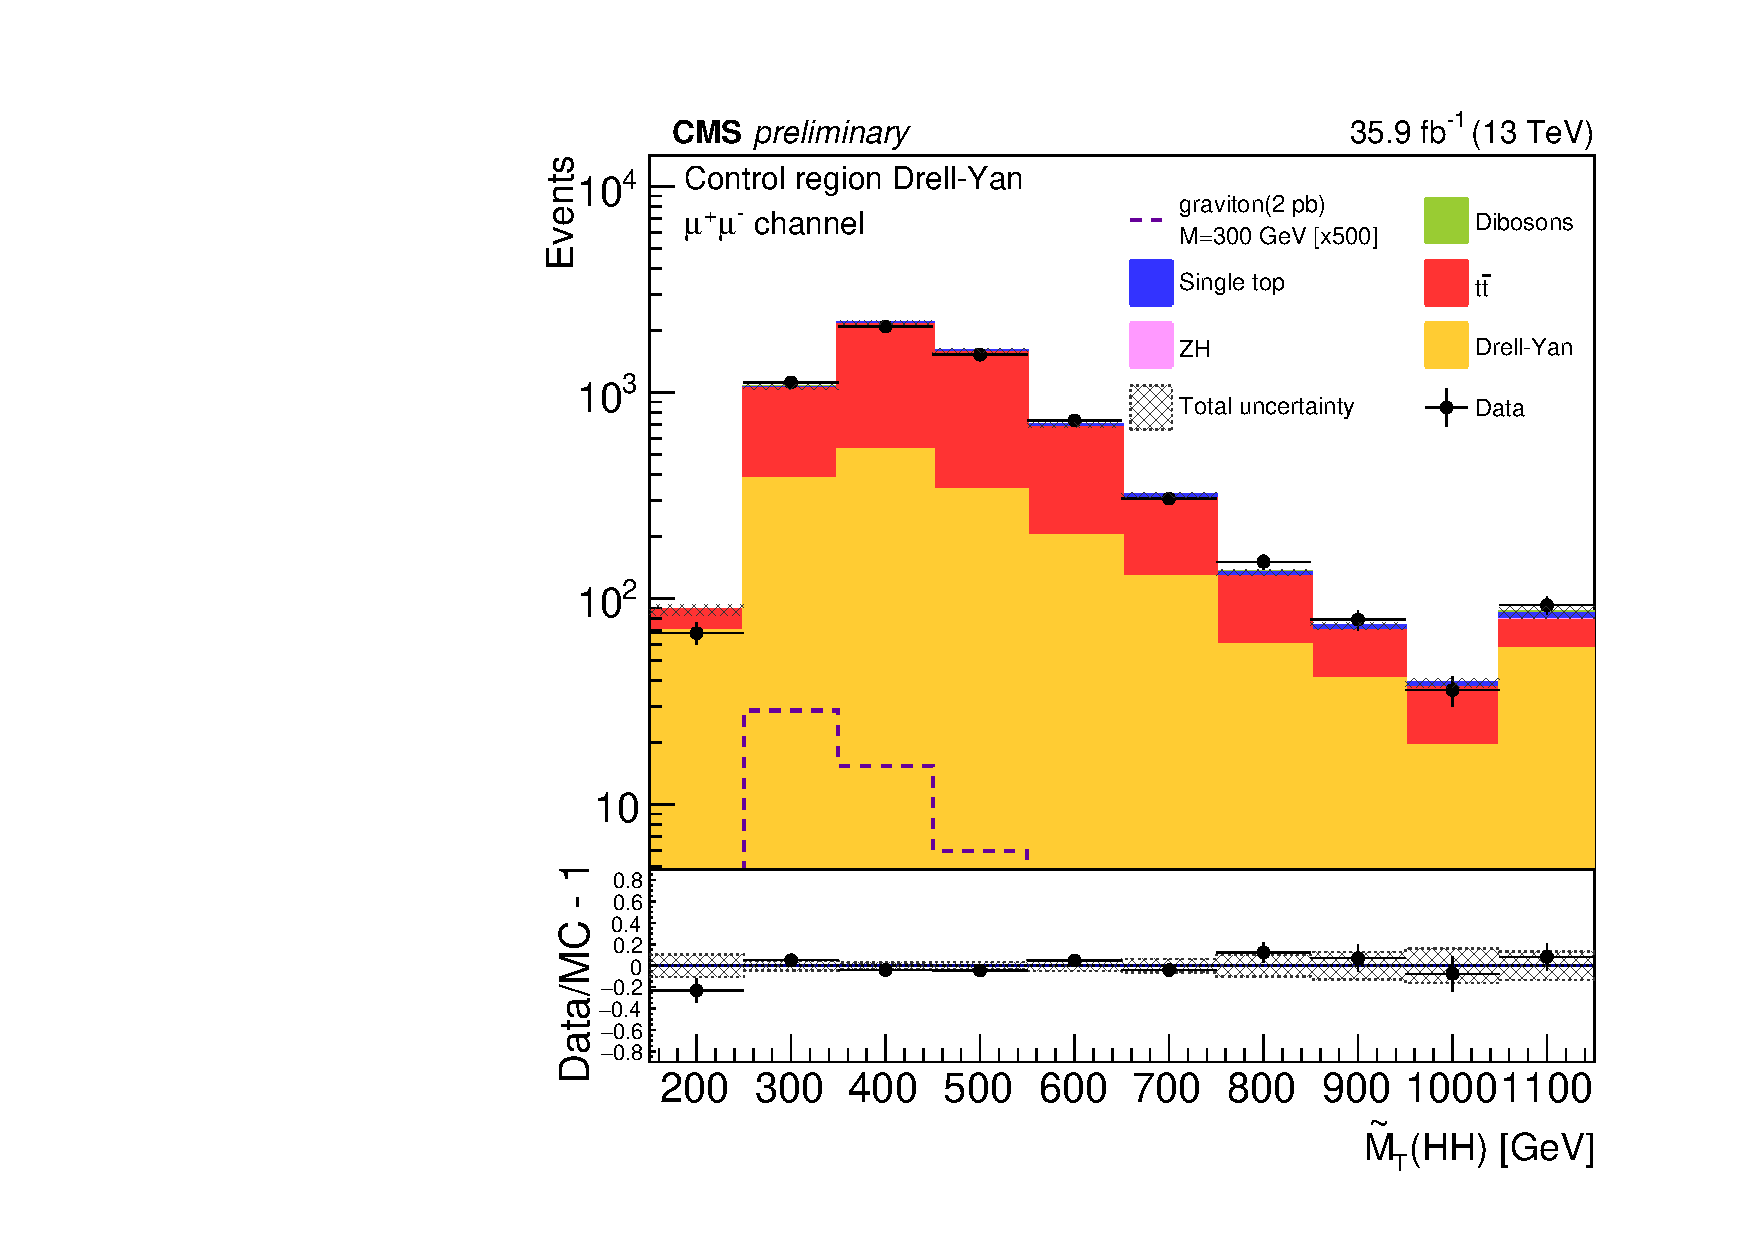
\includegraphics[width=0.31\textwidth]{hhMt_mm_CRDY_FullPostfit_plot_nov16_2_graviton.pdf}
    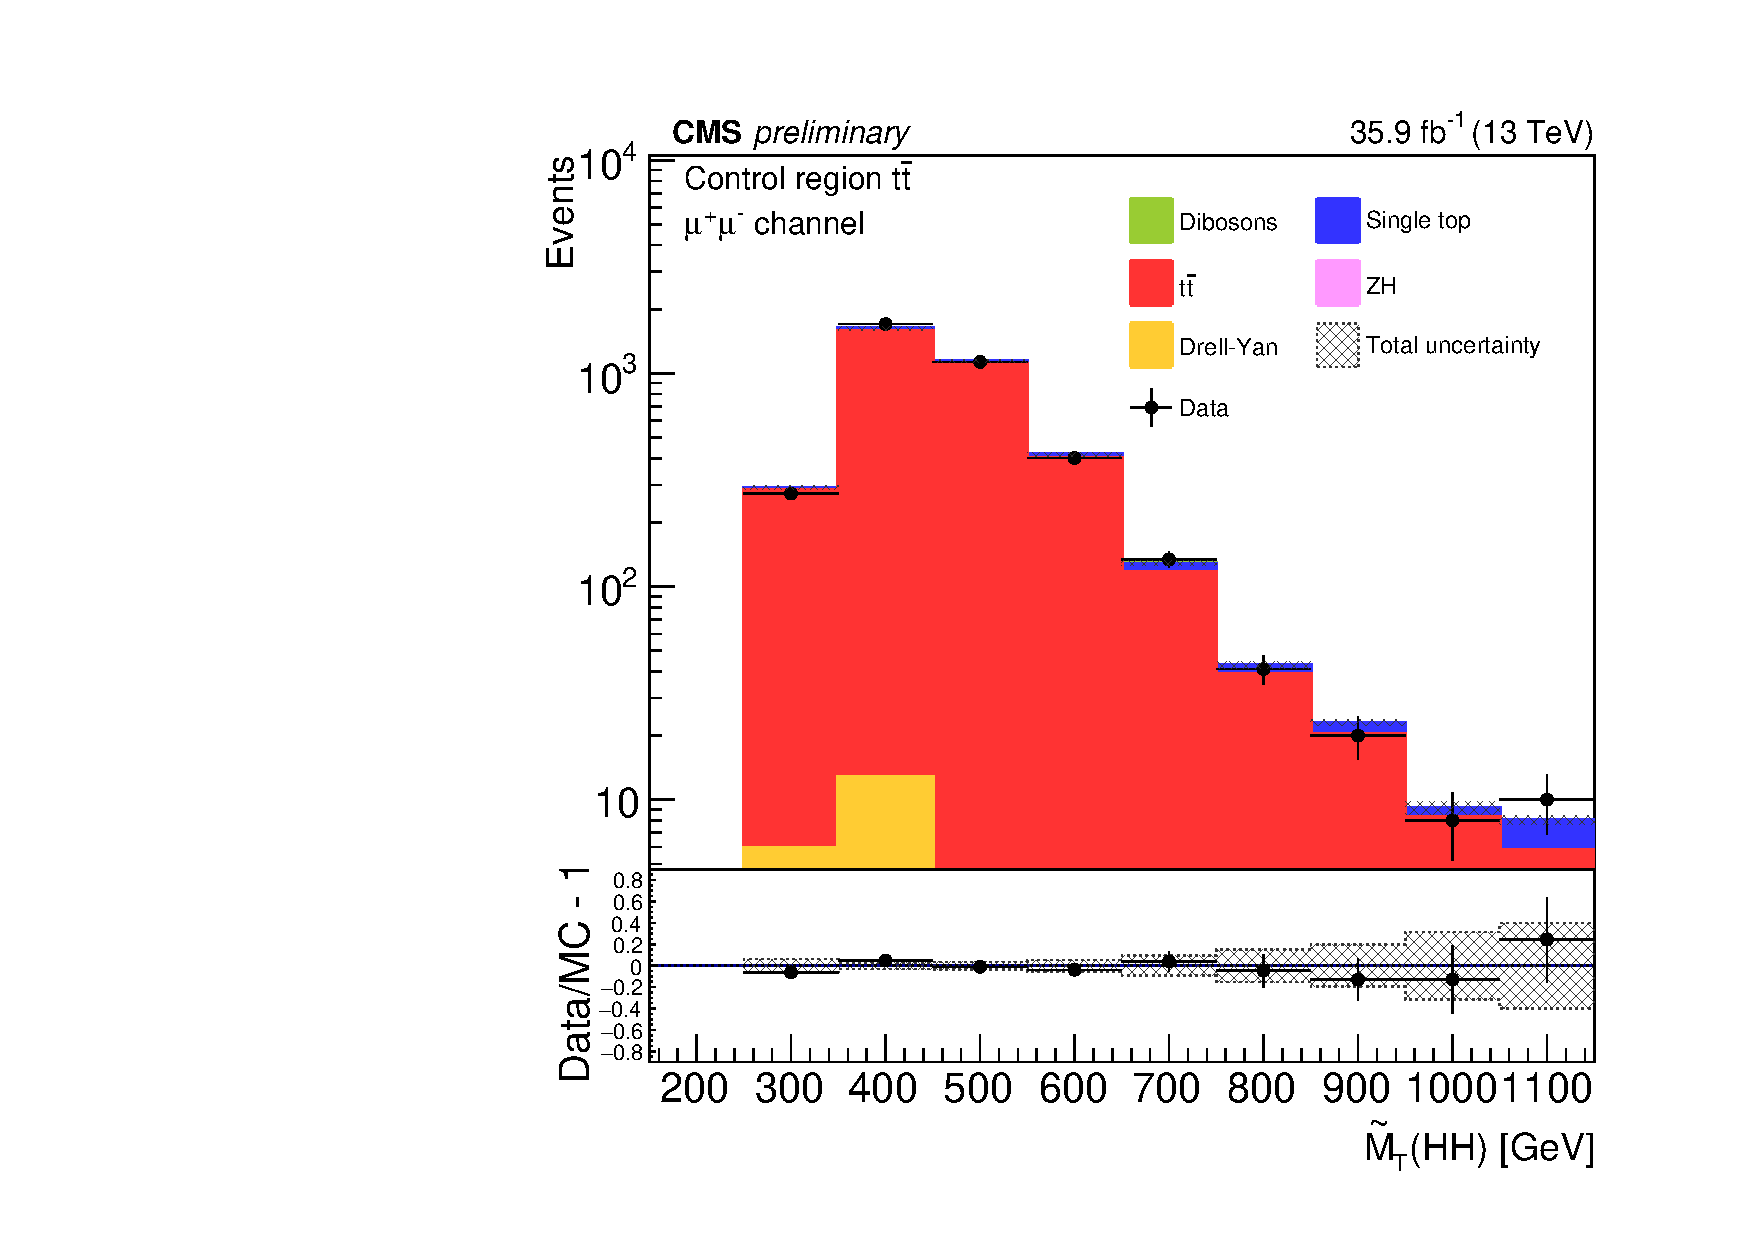
\includegraphics[width=0.31\textwidth]{hhMt_mm_CRTT_FullPostfit_plot_nov16_2_graviton.pdf}
    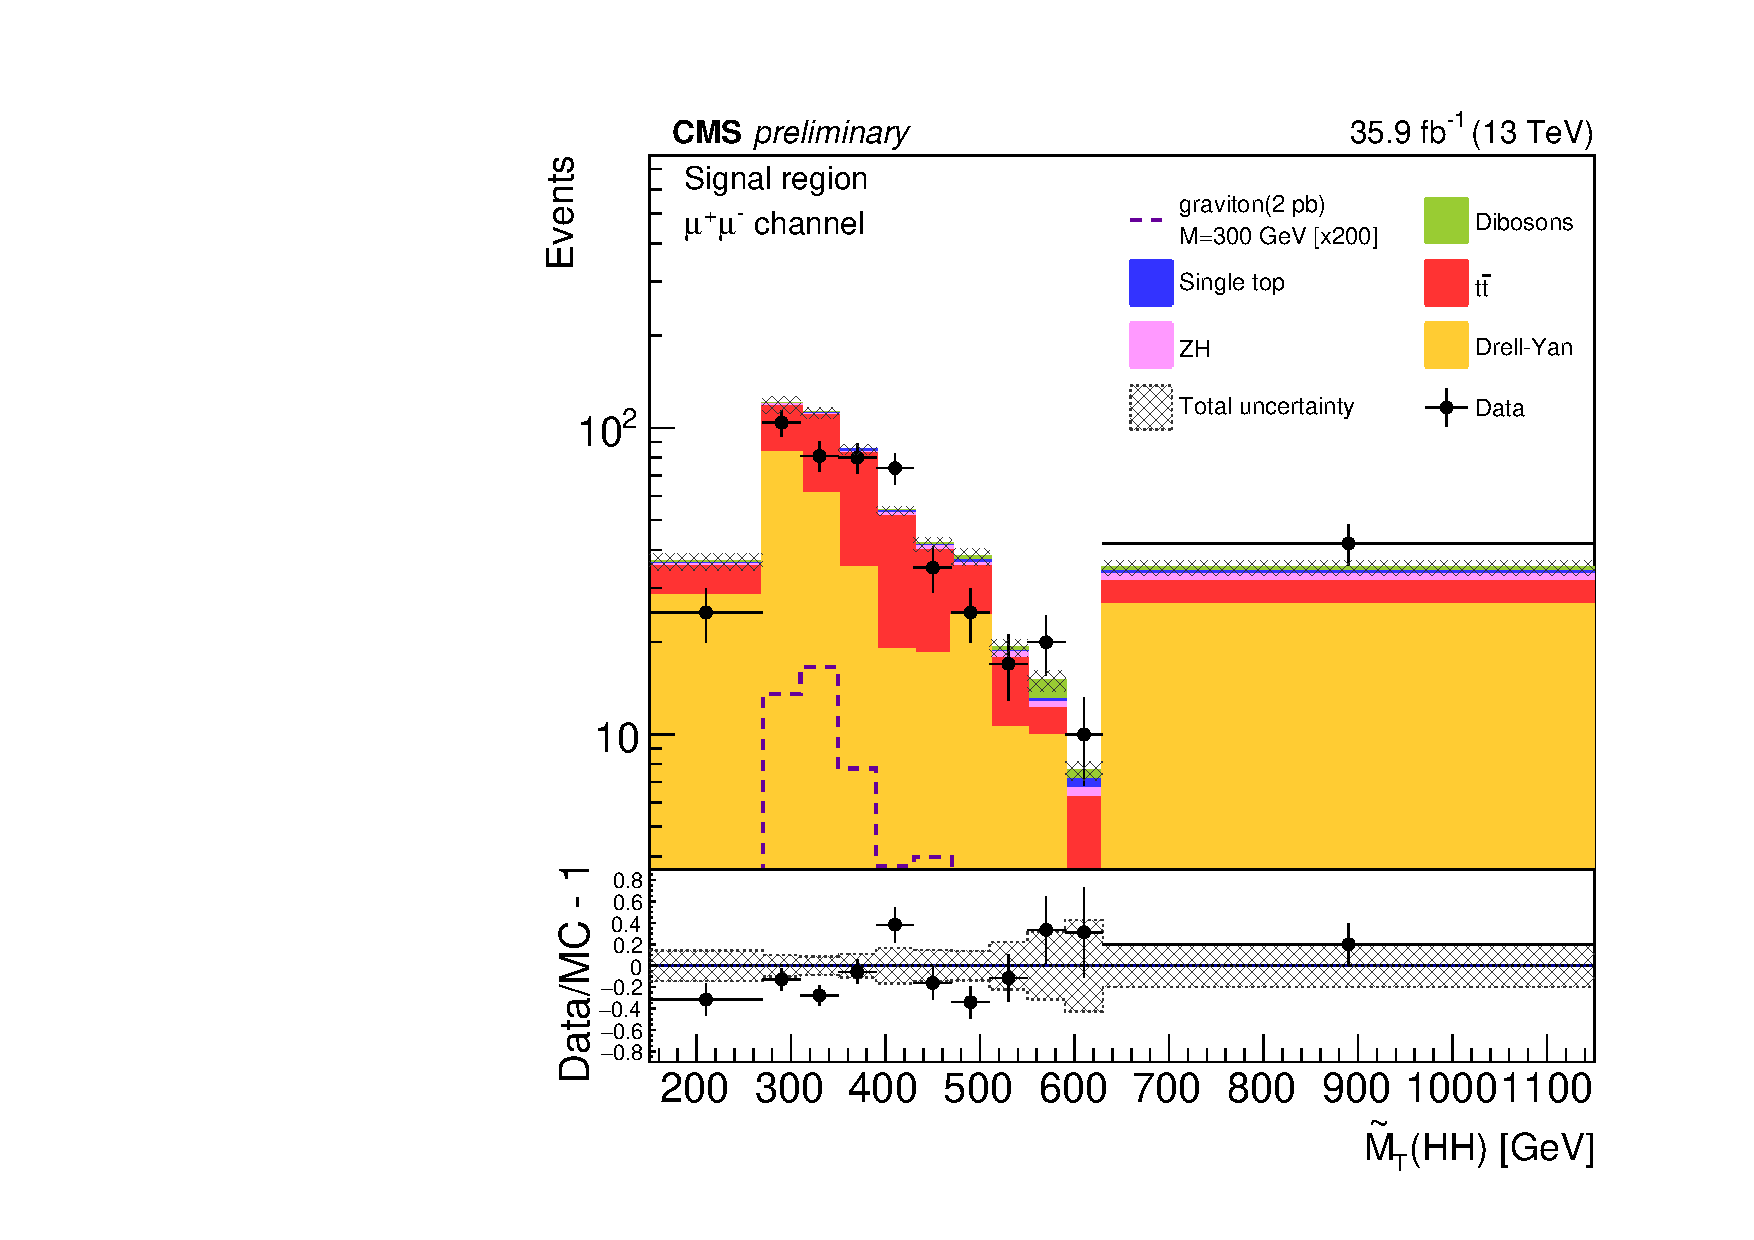
\includegraphics[width=0.31\textwidth]{hhMt_mm_SR_FullPostfit_plot_nov16_2_graviton.pdf} \\
    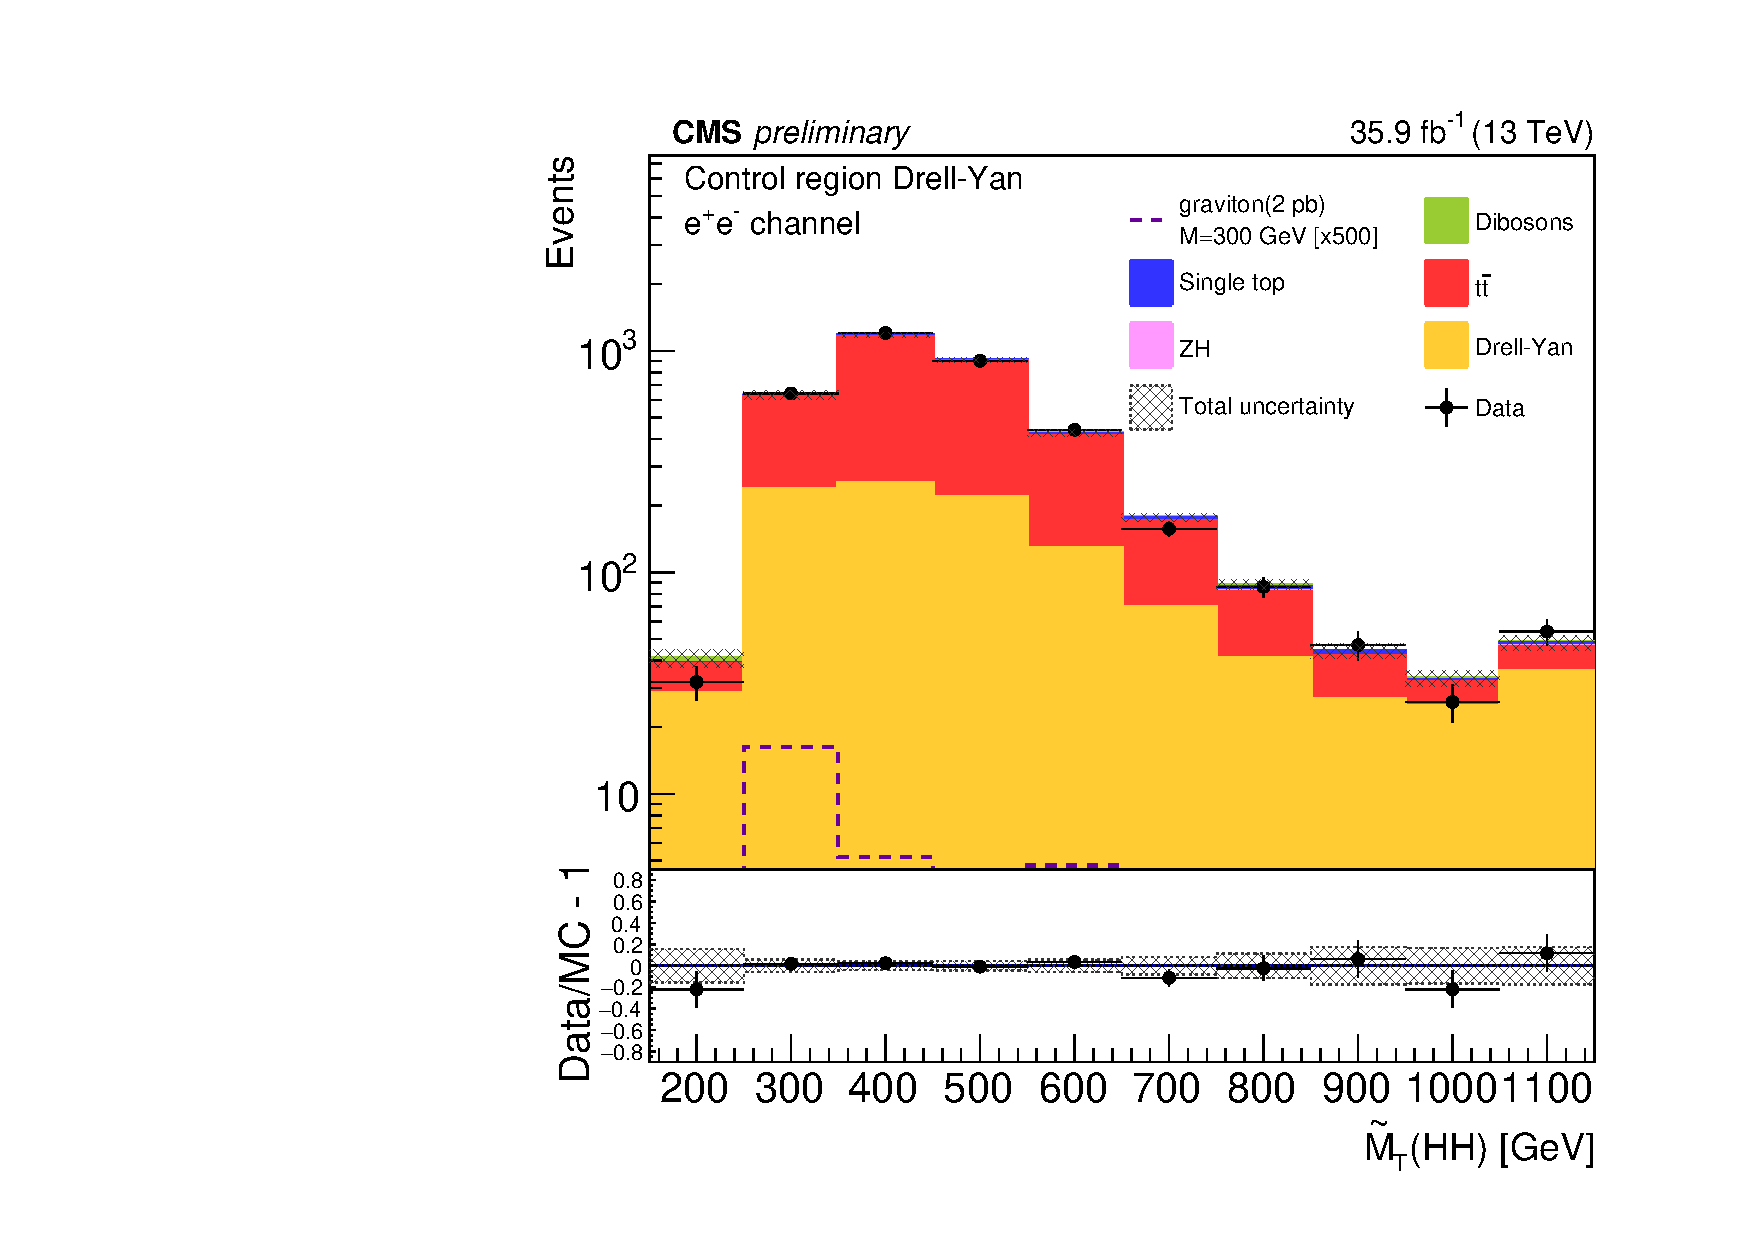
\includegraphics[width=0.31\textwidth]{hhMt_ee_CRDY_FullPostfit_plot_nov16_2_graviton.pdf}
    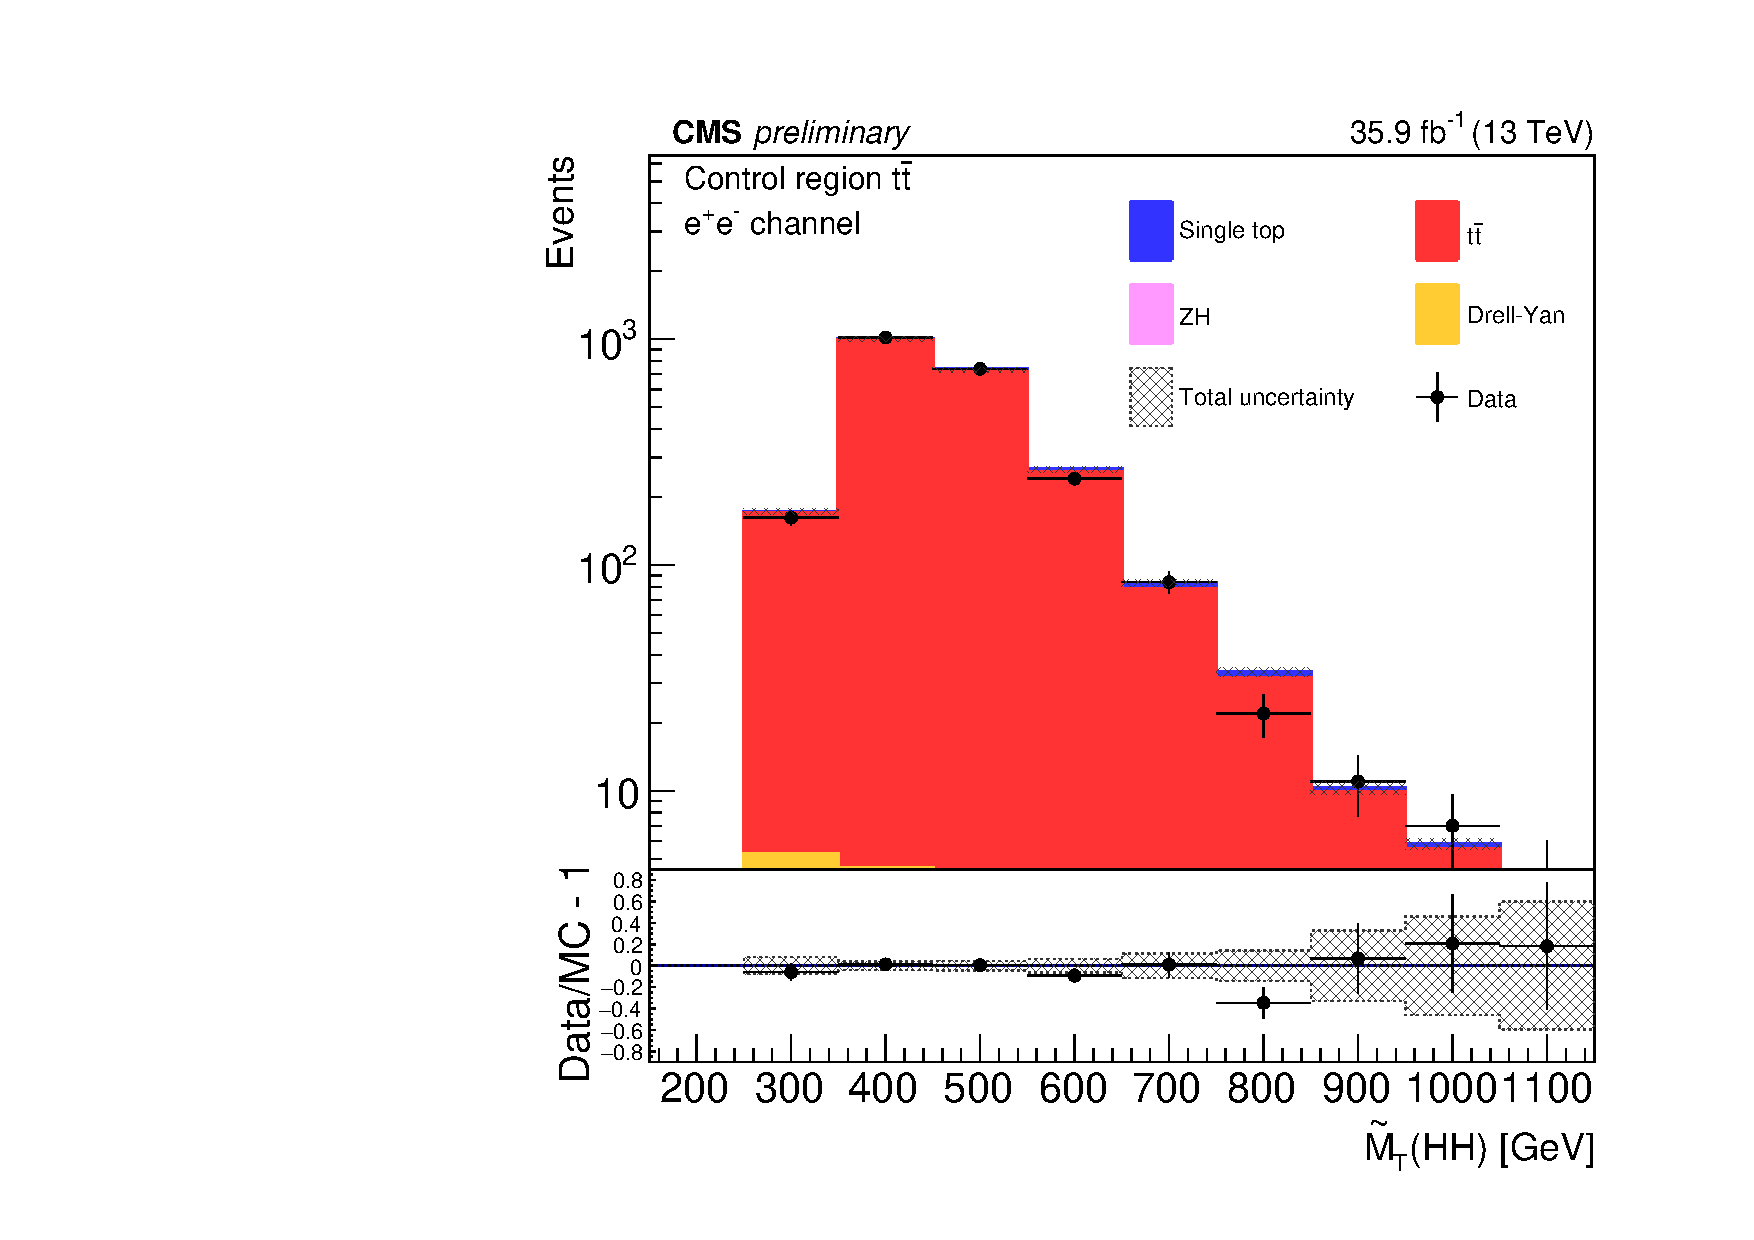
\includegraphics[width=0.31\textwidth]{hhMt_ee_CRTT_FullPostfit_plot_nov16_2_graviton.pdf}
    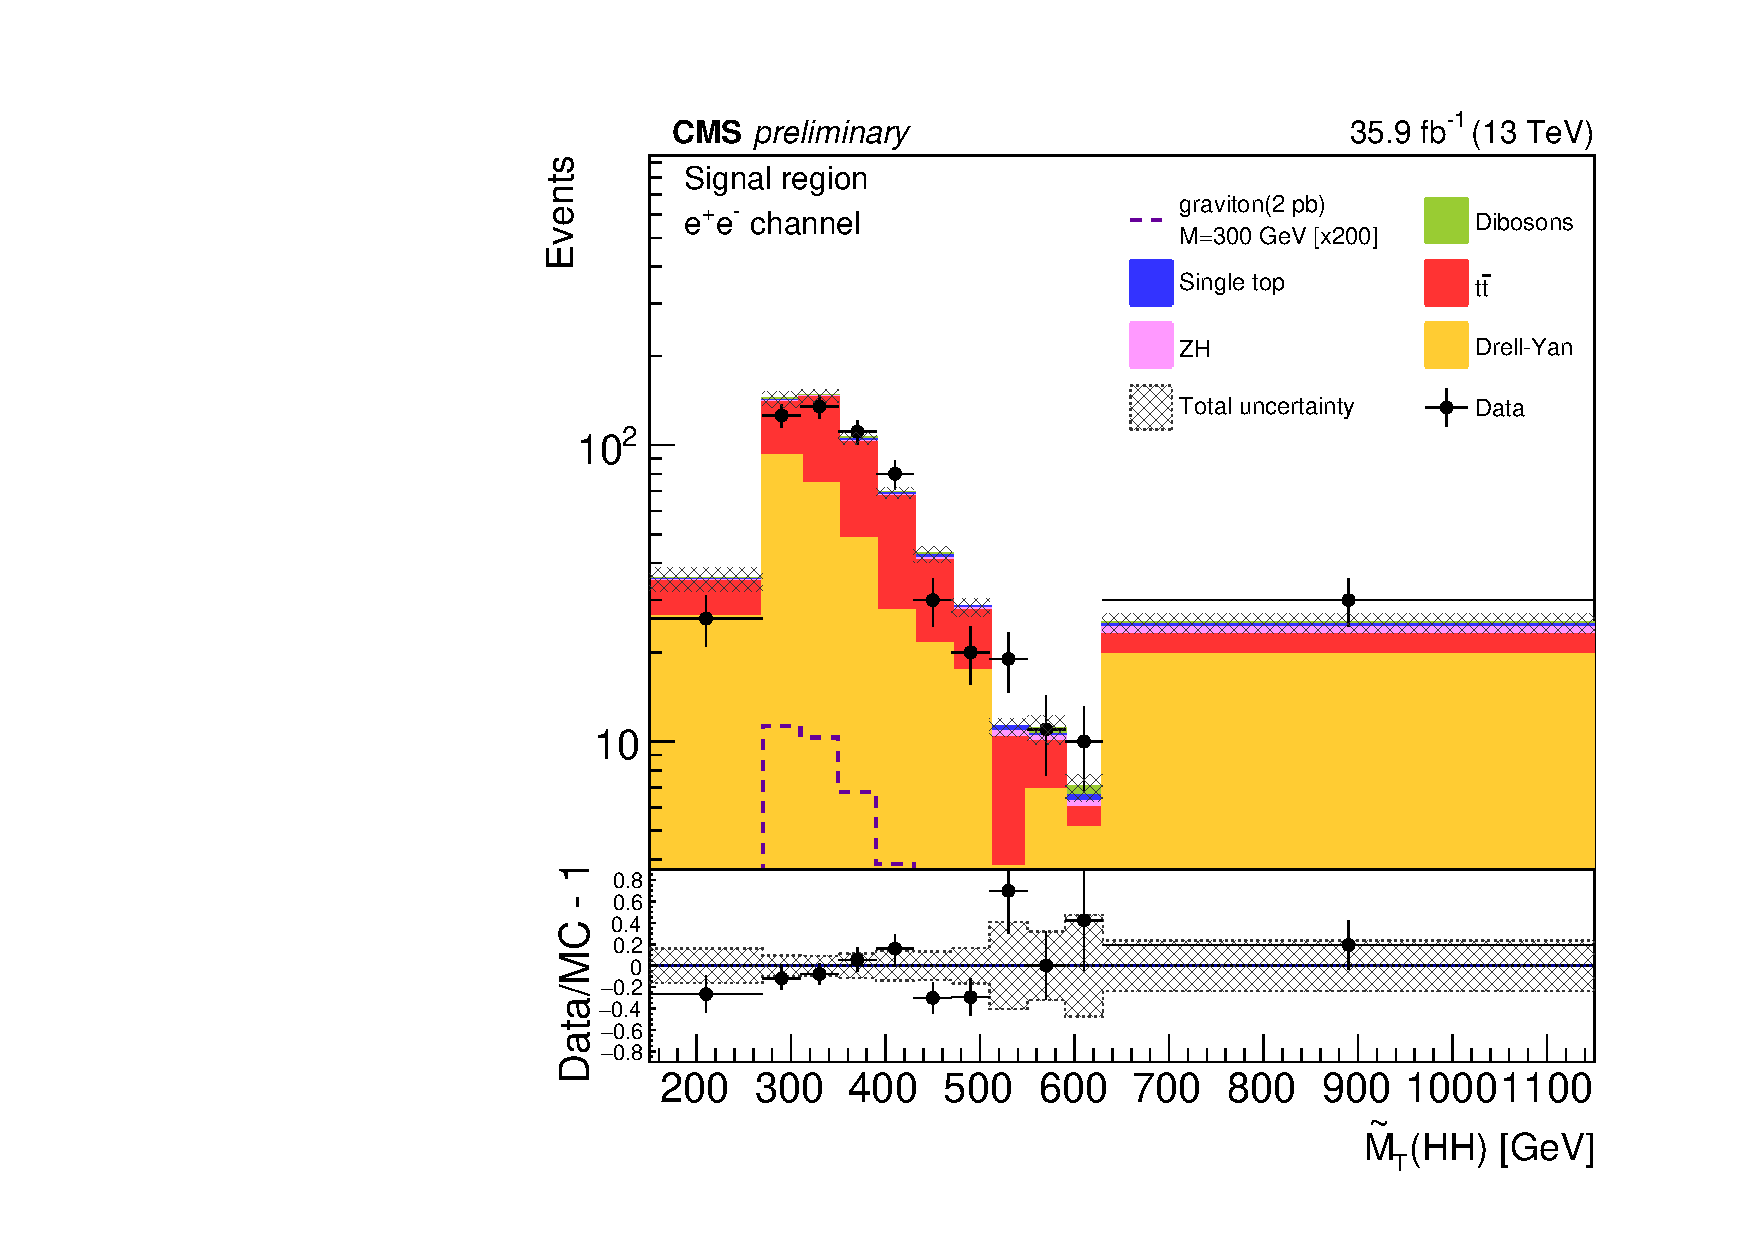
\includegraphics[width=0.31\textwidth]{hhMt_ee_SR_FullPostfit_plot_nov16_2_graviton.pdf}
    \caption{Transverse mass of the reconstructed HH candidates for data, the simulated signal graviton sample
    for the 300 GeV mass hypothesis, and simulated backgrounds scaled according to the fit results. The top
    row shows the figures for the muon channel while the bottom row is for the electron channel. For each row,
    the left plot is for the Drell-Yan control region, the middle is for the \ttbar control region, and the right
    is for the signal region. Signal normalization choice is discussed in the text. The crosshatched area represe\
nts
    the sum of statistical and systematic uncertainties.}
    \label{fig:MCcomparisons}
%                                                                                                                 
% Comparison of data and simulation.  Transverse mass of                                                          
%      the reconstructed HH candidate for 300 GeV signal mass                                                     
%      hypothesis, electron channel. Left: Drell-Yan control region. Middle: \ttbar                               
%      control region. Right: signal region. }                                                                    
%    \label{MCcomparisons_electrons}                                                                              
  \end{center}
\end{figure}




\begin{figure}[tbp]
  \begin{center}
    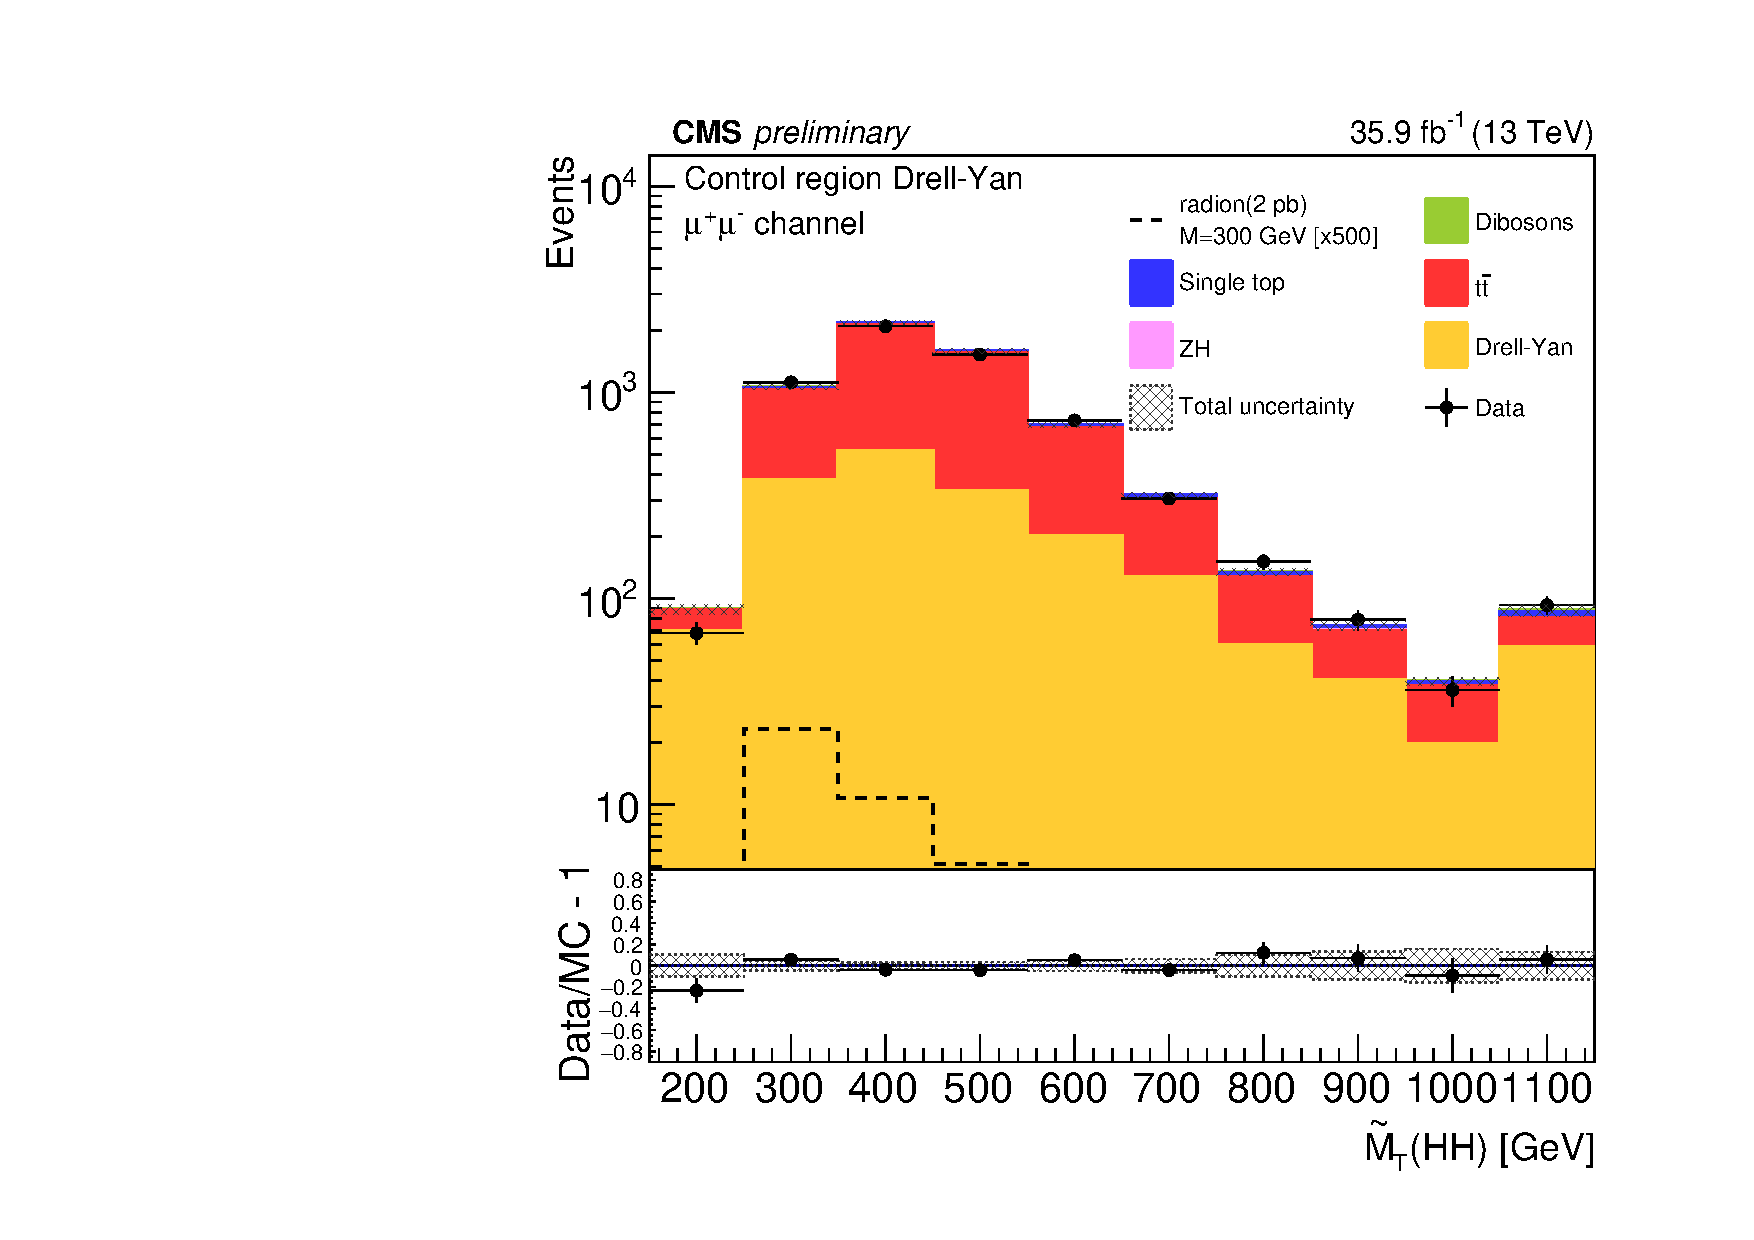
\includegraphics[width=0.31\textwidth]{hhMt_mm_CRDY_FullPostfit_plot_nov16_2_radion.pdf}
    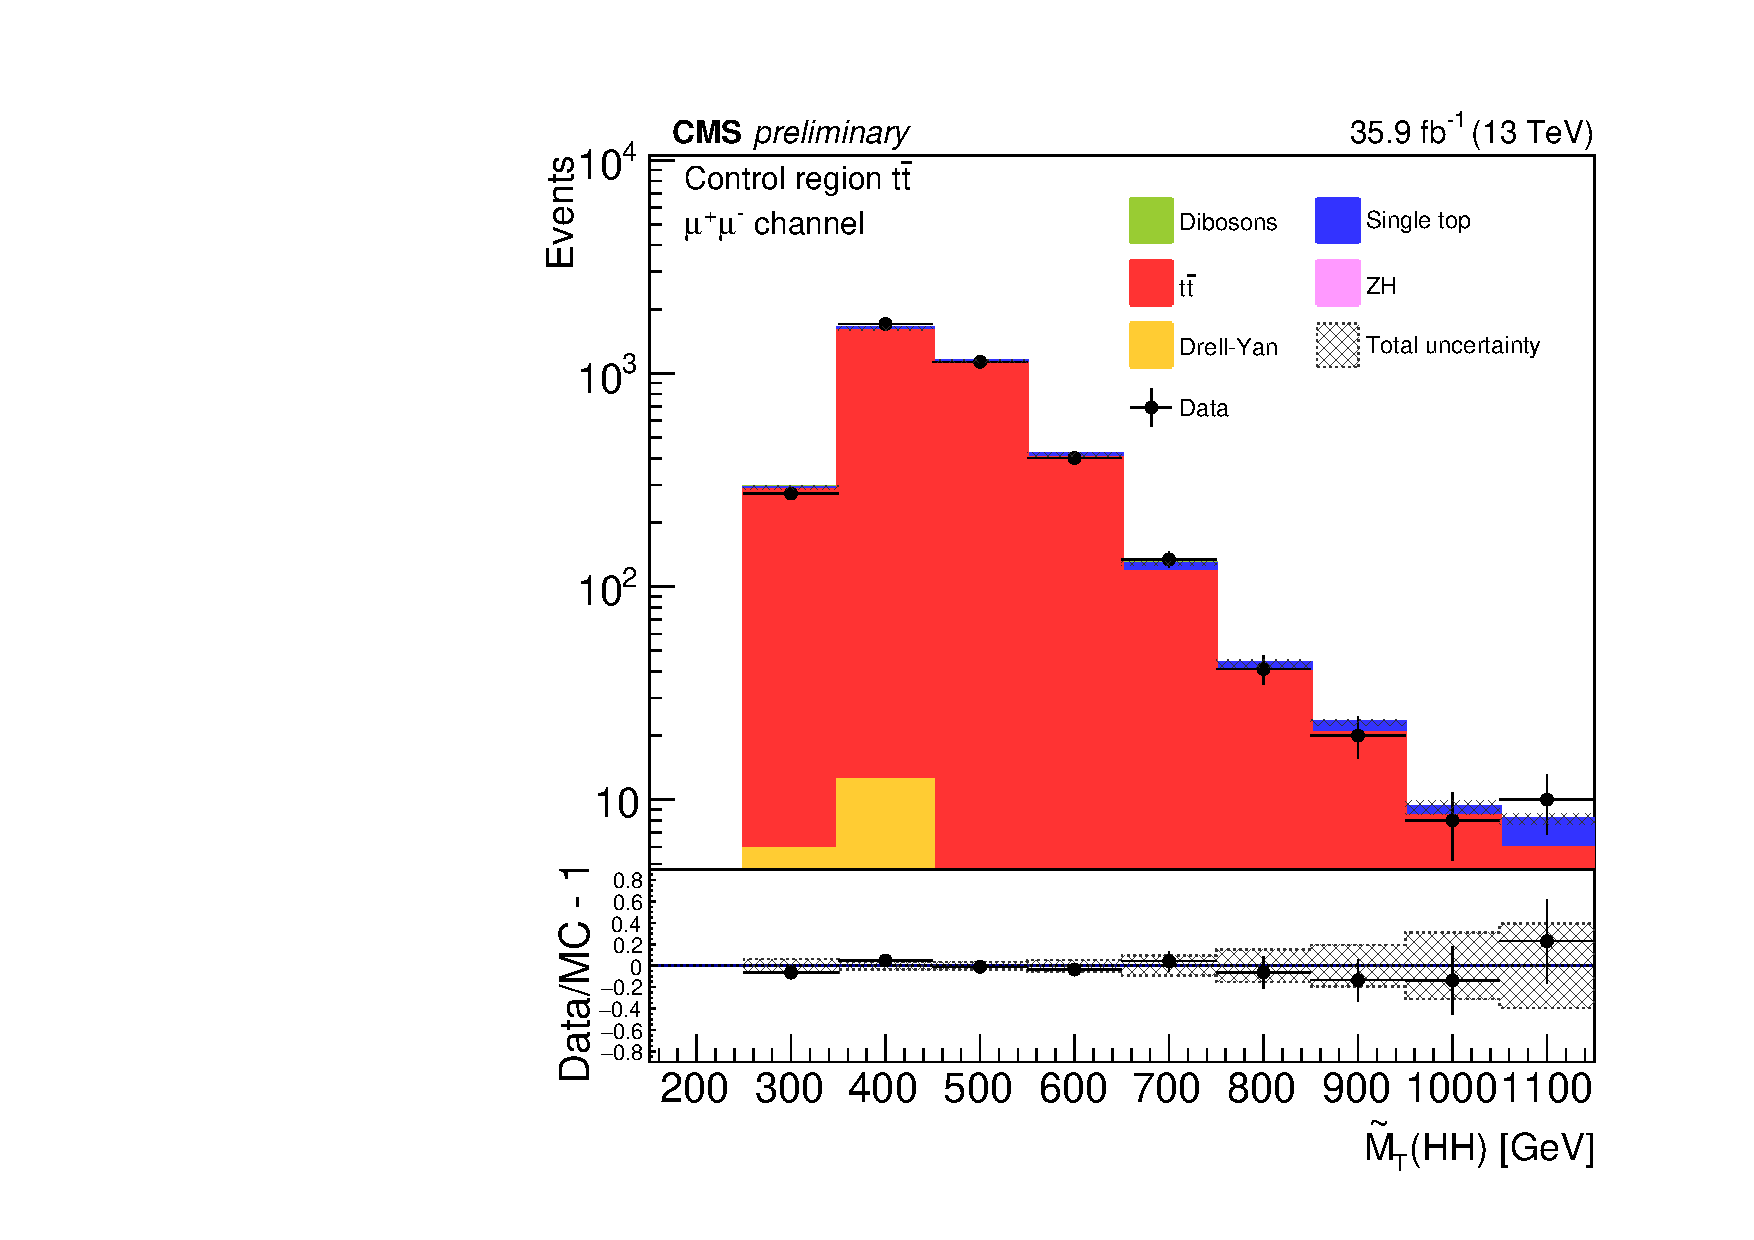
\includegraphics[width=0.31\textwidth]{hhMt_mm_CRTT_FullPostfit_plot_nov16_2_radion.pdf}
    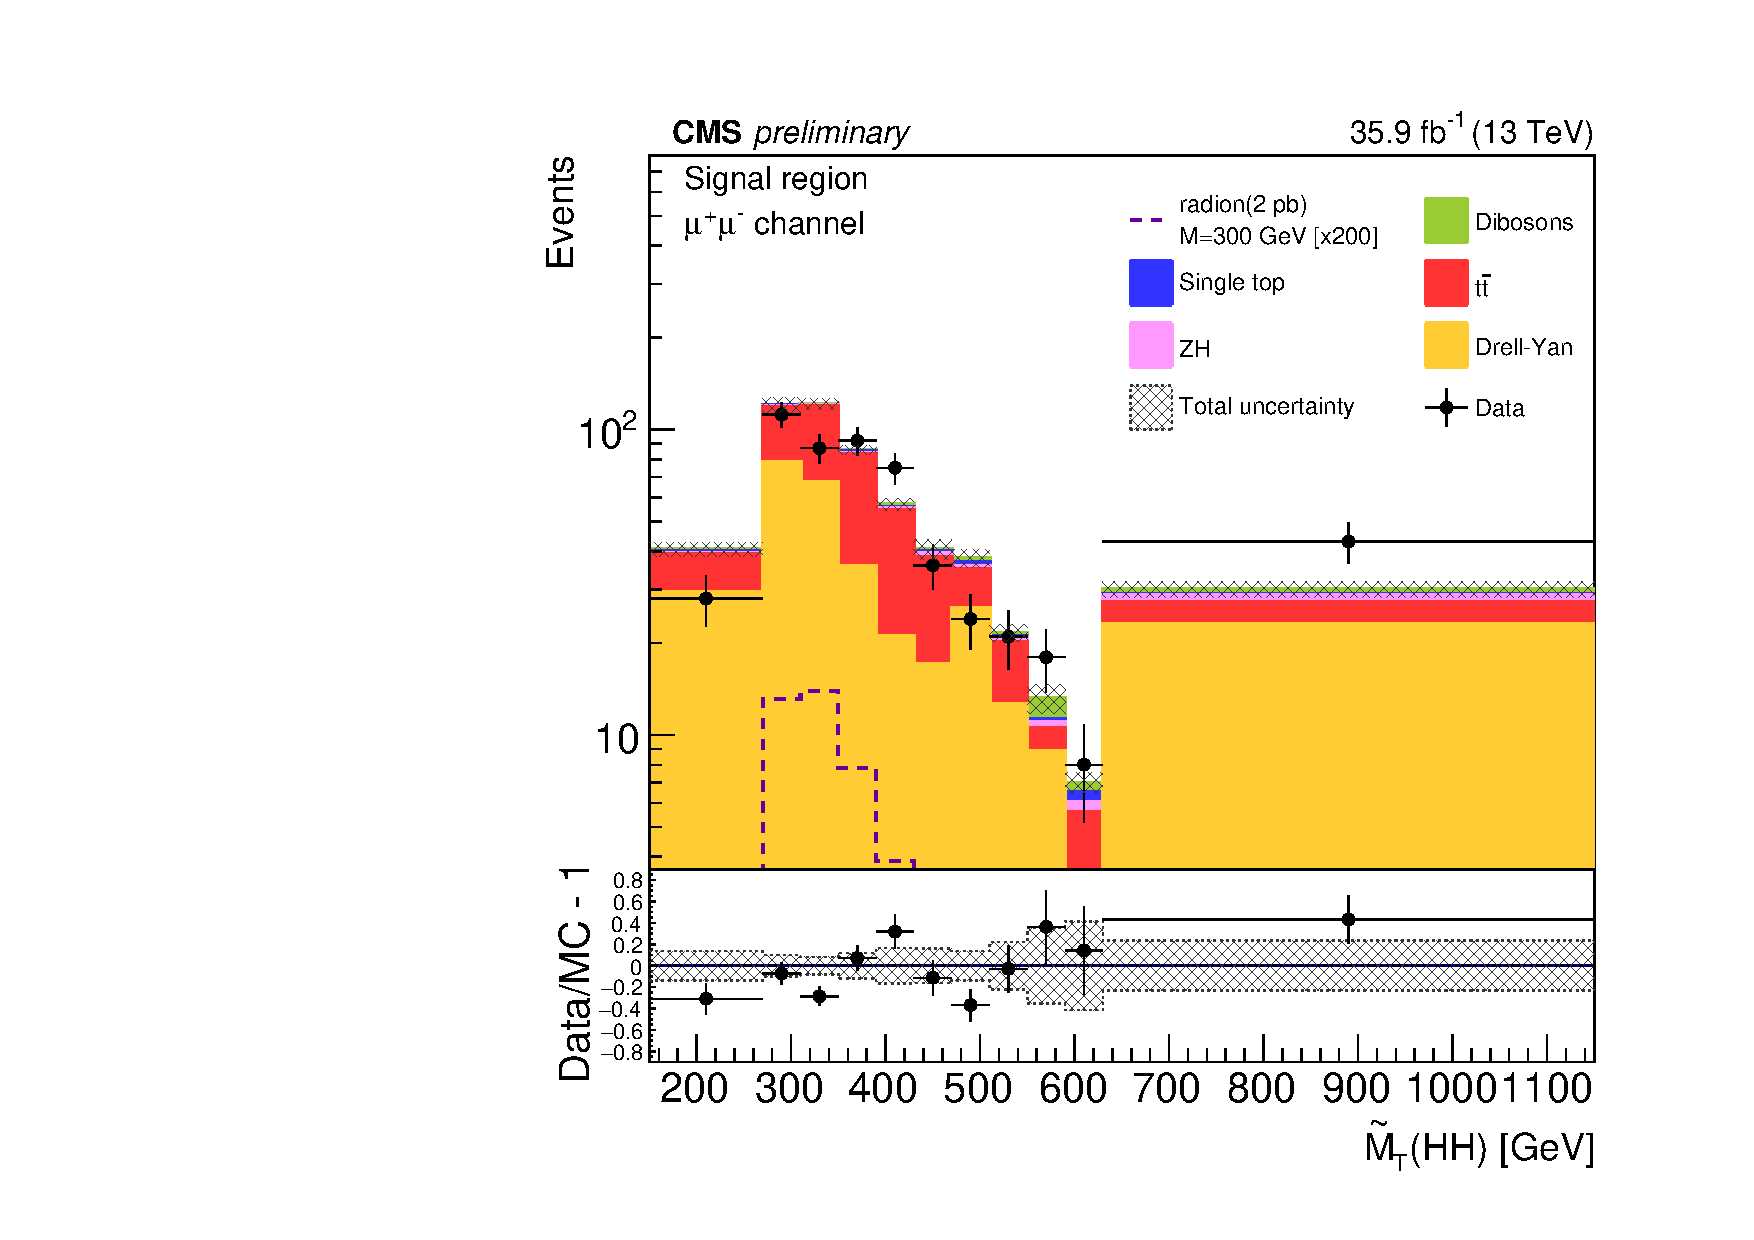
\includegraphics[width=0.31\textwidth]{hhMt_mm_SR_FullPostfit_plot_nov16_2_radion.pdf} \\
    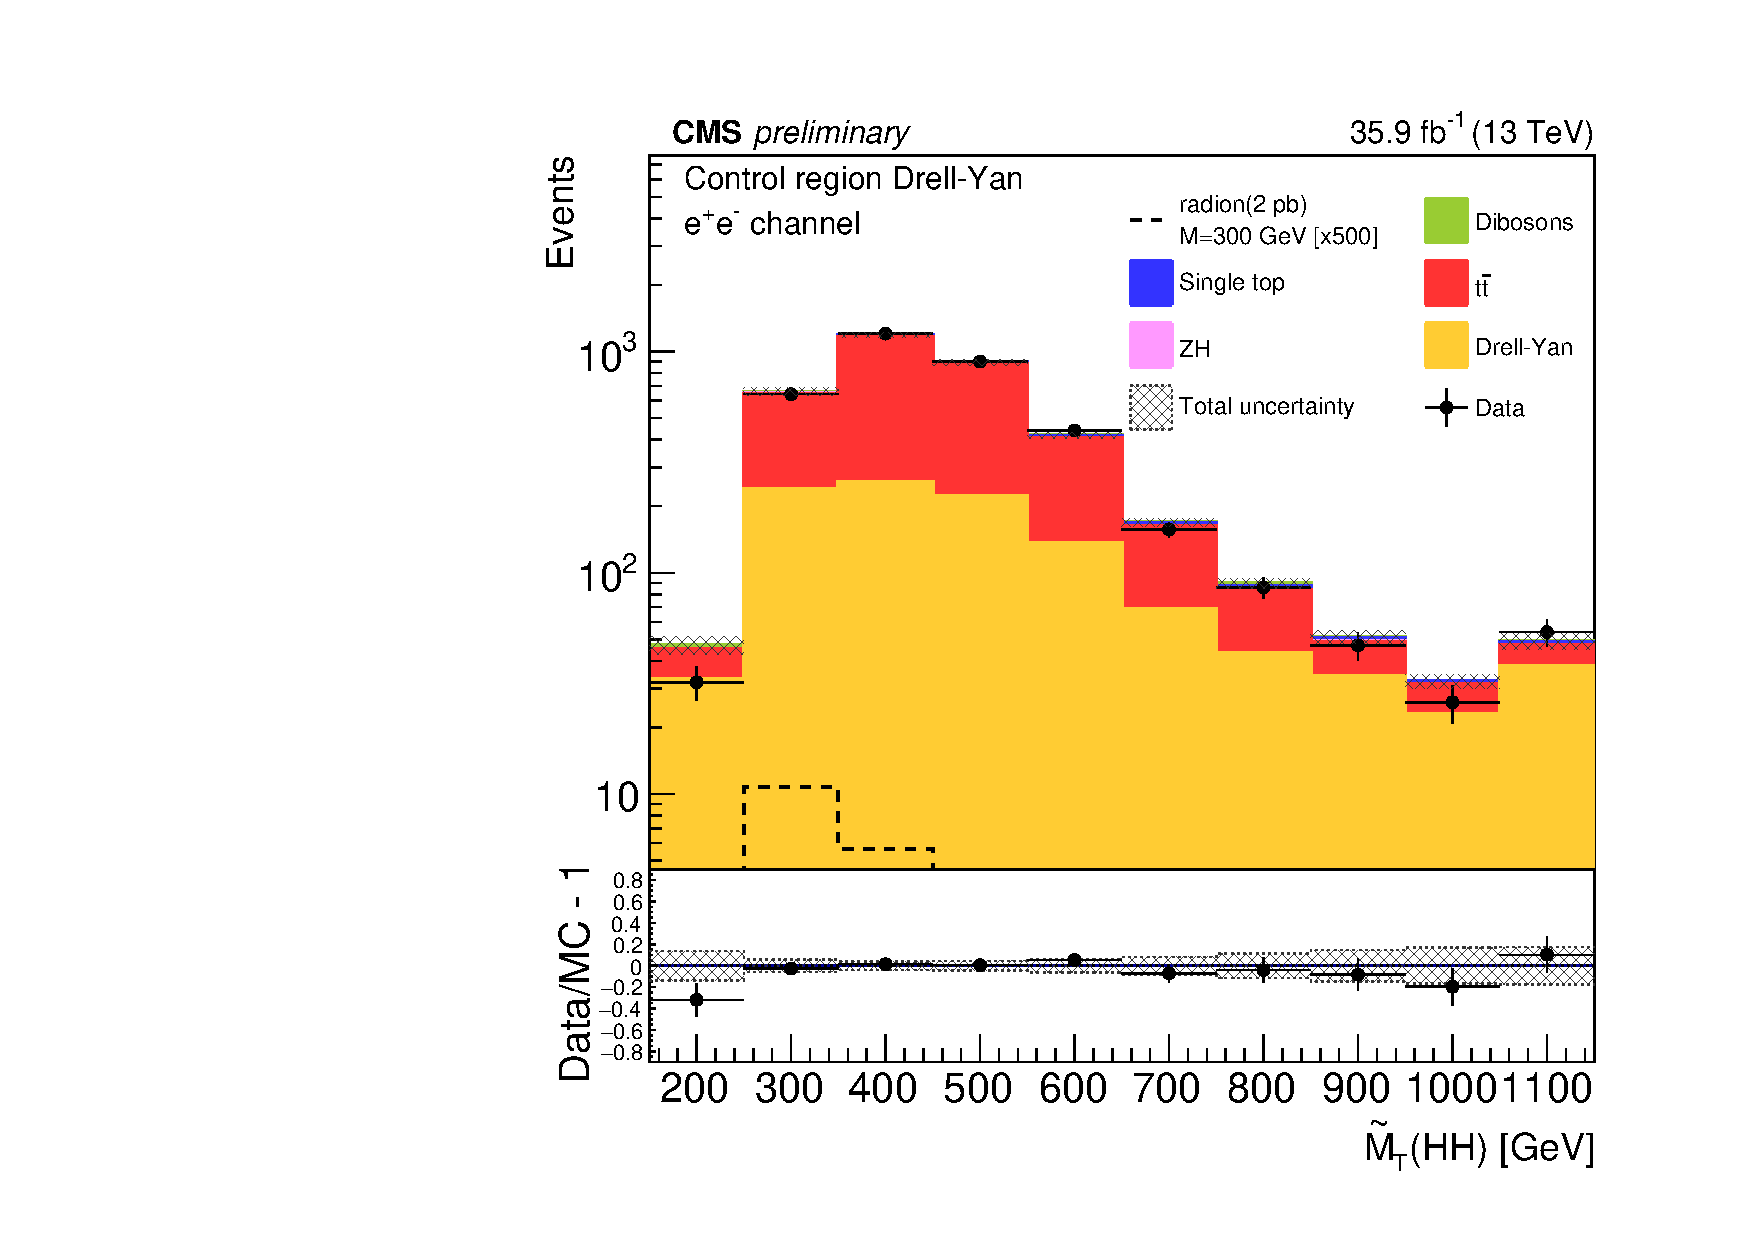
\includegraphics[width=0.31\textwidth]{hhMt_ee_CRDY_FullPostfit_plot_nov16_2_radion.pdf}
    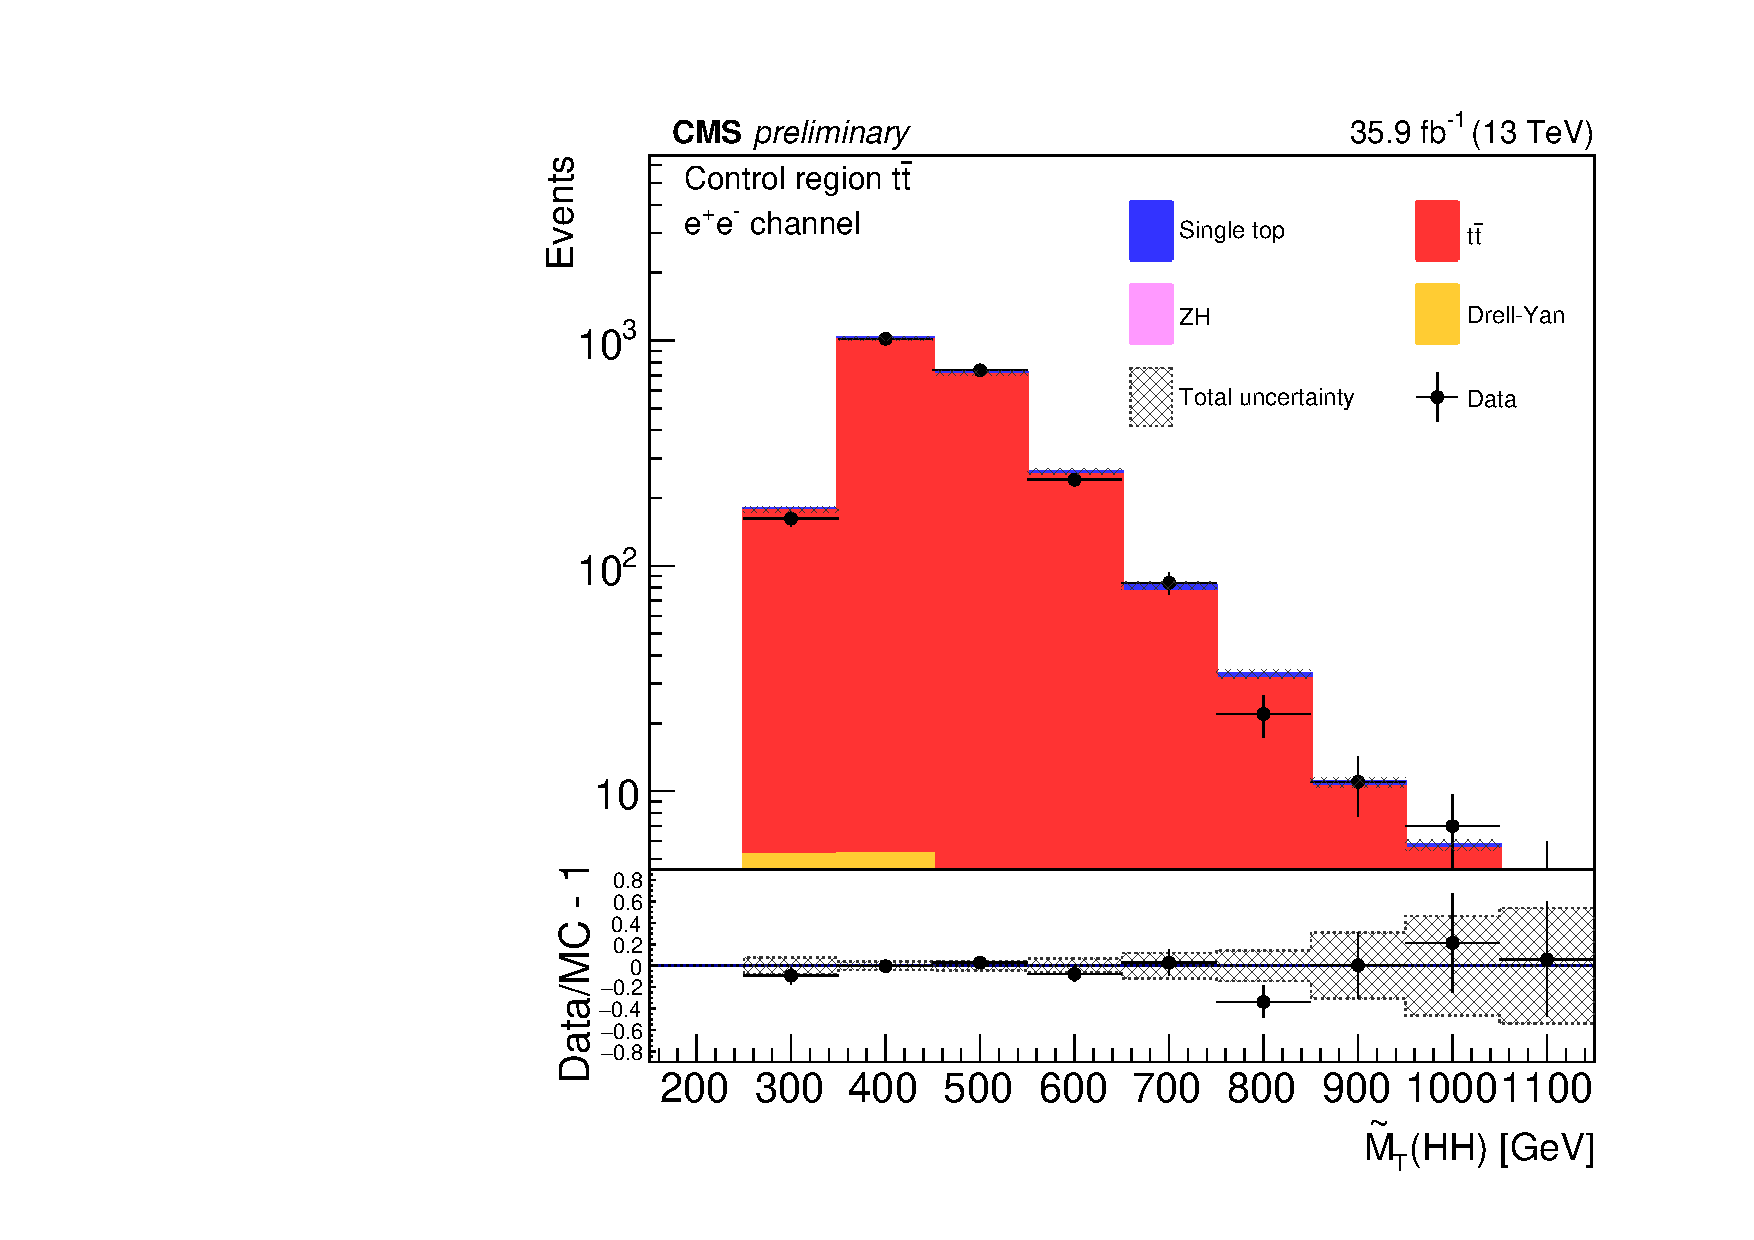
\includegraphics[width=0.31\textwidth]{hhMt_ee_CRTT_FullPostfit_plot_nov16_2_radion.pdf}
    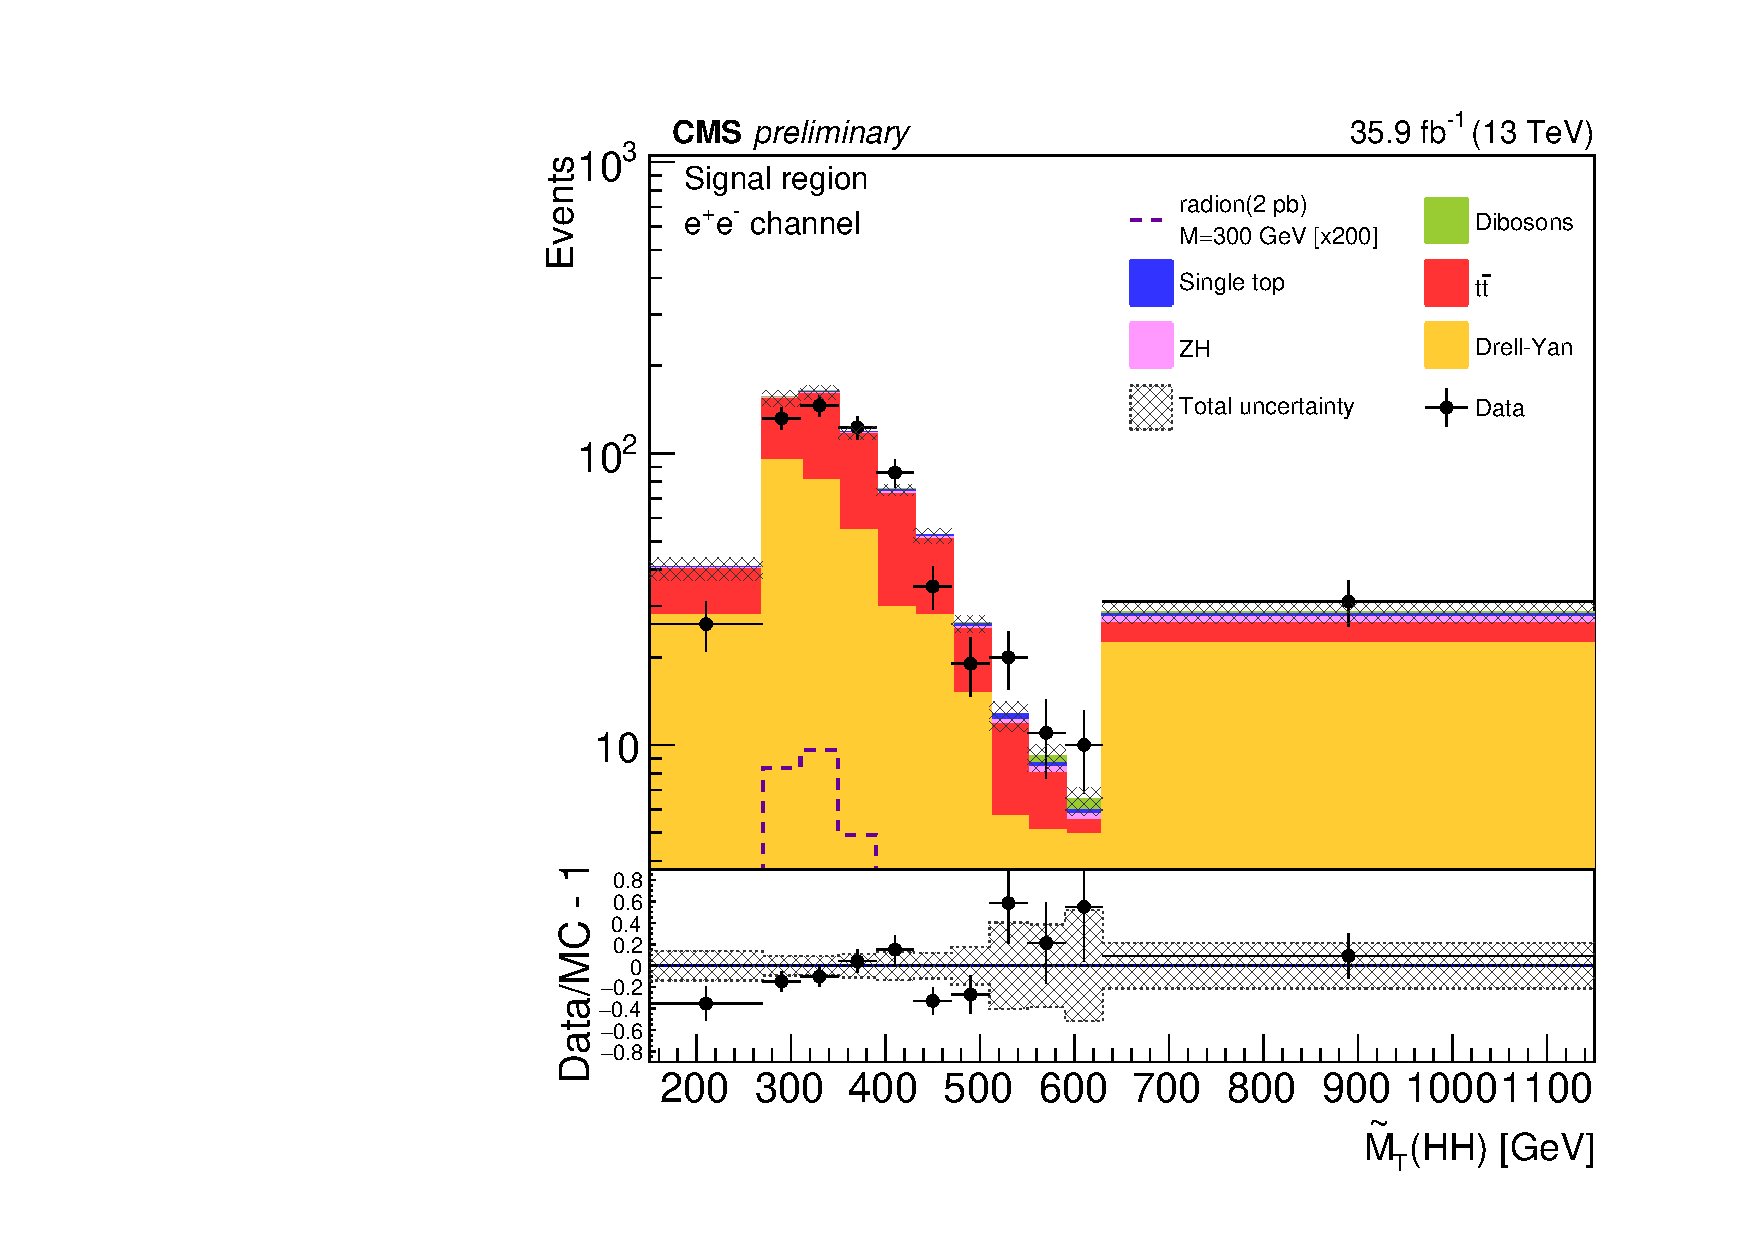
\includegraphics[width=0.31\textwidth]{hhMt_ee_SR_FullPostfit_plot_nov16_2_radion.pdf}
    \caption{Transverse mass of the reconstructed HH candidates for data, the simulated signal radion sample
    for the 300 GeV mass hypothesis, and simulated backgrounds scaled according to the fit results. The top
    row shows the figures for the muon channel while the bottom row is for the electron channel. For each row,
    the left plot is for the Drell-Yan control region, the middle is for the \ttbar control region, and the right
    is for the signal region. Signal normalization choice is discussed in the text. The crosshatched area represe\
nts
    the sum of statistical and systematic uncertainties.}
    \label{fig:MCcomparisons_radion}
%                                                                                                                 
% Comparison of data and simulation.  Transverse mass of                                                          
%      the reconstructed HH candidate for 300 GeV signal mass                                                     
%      hypothesis, electron channel. Left: Drell-Yan control region. Middle: \ttbar                               
%      control region. Right: signal region. }                                                                    
%    \label{MCcomparisons_electrons}                                                                              
  \end{center}
\end{figure}





%are presented (See Figs.  ~\ref{fig:MCcomparisons_ee_low_SR_bdt_sideband}, ~\ref{fig:MCcomparisons_ee_low_SR_bdt_sideband_2}, ~\ref{fig:MCcomparisons_ee_low_CRDY}, ~\ref{fig:MCcomparisons_ee_low_CRDY_2}, ~\ref{fig:MCcomparisons_ee_low_CRTT}, ~\ref{fig:MCcomparisons_ee_low_CRTT_2} . Unblinded ee distributions are shown in the Fig. ~\ref{fig:MCcomparisons_ee_low_SR}, ~\ref{fig:MCcomparisons_ee_low_SR_2}.
%Muon channel plots are also shown.(See Figs. ~\ref{fig:MCcomparisons_mm_low_SR_bdt_sideband}, ~\ref{fig:MCcomparisons_mm_low_SR_bdt_sideband_2}, ~\ref{fig:MCcomparisons_mm_low_CRDY}, ~\ref{fig:MCcomparisons_mm_low_CRDY_2}, ~\ref{fig:MCcomparisons_mm_low_CRTT}, ~\ref{fig:MCcomparisons_mm_low_CRTT_2}.  Unblinded mm distributions are shown in the Fig. ~\ref{fig:MCcomparisons_mm_low_SR}, ~\ref{fig:MCcomparisons_mm_low_SR_2}.

%BDT plots for all mass hypotheses for SR can be found on the Fig. ~\ref{fig:bdt_ee_SR} for electron channel and ~\ref{fig:bdt_mm_SR} for the muon channel. BDT distributions in CRDY and CRTT for electon channel are shown on the Figs. ~\ref{fig:bdt_ee_CRDY}, ~\ref{fig:bdt_ee_CRTT}, and for muon channel on the Figs.  ~\ref{fig:bdt_mm_CRDY}, ~\ref{fig:bdt_mm_CRTT}.

%BDT plots in the case of electrons are shown at ~\ref{fig:bdt_ee} and in case case of muons at ~\ref{fig:bdt_mm}.
% for the muon channel. BDT distributions in CRDY and CRTT for electon channel are shown on the Figs. ~\ref{fig:bdt_ee_CRDY}, ~\ref{fig:bdt_ee_CRTT}, and for muon channel on the Figs.  ~\ref{fig:bdt_mm_CRDY}, ~\ref{fig:bdt_mm_CRTT}.


\subsubsection{Scale Factors}
%\subsubsection{HLT Lepton Scale Factors}

Electron ID and ISO scale factors, as well as HLT scale factors (Fig.~\ref{fig:trigger_eff_diele}), have been computed by VHbb group and presented at the EGamma physics object groups (POG) meeting~\cite{egSF}.
Muon ID scale factors, as well as ISO scale factors, have been derived separately for runs G/H and B/C/D/E/F runs and then luminosity averaged ~\cite{muonIDnISO}. Tracker scale factors (~\ref{fig:trigger_eff_diele}) are taken from the Muon POG twiki~\cite{muonTRK}. HLT dimuon scale factors were derived by VHbb group and further approved by the muon POG. These scale factors were derived separately for run H (Fig.~\ref{fig:trigger_SF_dimu_H}) and B/C/D/E/F/G (Fig.~\ref{fig:trigger_SF_dimu_BCDEFG}) runs and then luminosity averaged ~\cite{muonTrigger}. On top, separate scale factors are calculated for the dZ requirement of HLT\_Mu17\_TrkIsoVVL\_Mu8\_TrkIsoVV\
L\_DZ\_v* OR HLT\_Mu17\_TrkIsoVVL\_TkMu8\_TrkIsoVVL\_DZ\_v* triggers, using dilepton events that have already passed the HLT\_Mu17\_TrkIsoVVL\_Mu8\_TrkIsoVVL\_v*\
 OR HLT\_Mu17\_TrkIsoVVL\_TkMu8\_TrkIsoVVL\_v* triggers (Fig. ~\ref{fig:trigger_SF_dimu_dZ_H}).


\clearpage

\section{Background predictions}
\label{sec:backgrounds}
The modeling of reducible and irreducible backgrounds in this analysis uses the exact methods, analysis code, and ROOT trees used for the \ttH\ multilepton analysis which is being finalized concurrently.
We give a brief description of the methods and refer to the documentation of that analysis in Refs.~\cite{CMS_AN_2016-211,CMS_AN_2017-029} for any details.

The backgrounds in three-lepton and same-sign dilepton final states can be split in two broad categories: irreducible backgrounds with genuine prompt leptons (\ie\ from on-shell \PW\ and \Z\ boson decays); and reducible backgrounds where at least one of the leptons is ``non-prompt'', \ie\ produced within a hadronic jet, either a genuine lepton from heavy flavor decays, or simply mis-reconstructed jets.
A further class of reducible backgrounds consists of leptons with a mis-reconstructed electric charge sign, only truly relevant for electrons.

Irreducible backgrounds can be reliantly estimated directly from Monte-Carlo simulated events, using higher-order cross sections or data control regions for the overall normalization.
This is done in this analysis for all backgrounds involving prompt leptons: \ttW, \ttZ, \ttH, \WZ, $\Z\Z$, $\PW^\pm\PW^\pm\cPq\cPq$, $\cPqt\cPaqt\cPqt\cPaqt$, $\cPqt\Z\cPq$, $\cPqt\Z\PW$, $\PW\PW\PW$, $\PW\PW\Z$, $\PW\Z\Z$, $\Z\Z\Z$.

Reducible backgrounds, on the other hand, are not well predicted by simulation, and are estimated using data-driven methods.
In the case of non-prompt leptons, a fake rate method is used where the contribution to the final selection is estimated by extrapolating from a sideband (or ``application region'') with a looser lepton definition (the fakeable object definitions in Tabs.~\ref{tab:muonIDs} and~\ref{tab:eleIDs}) to the signal selection.
The tight-to-loose ratios (or ``fake rates'') are measured in several background dominated data events with dedicated triggers, subtracting the residual prompt lepton contribution using MC.\@
Non-prompt leptons in our signal regions are predominantly produced in \ttbar\ events, with a much smaller contribution, mainly in the three-lepton channel, from Drell--Yan production.
The systematic uncertainty on the normalization of the non-prompt background estimation is on the order of 50\%, and thereby one of the dominant limitations on the performance of multilepton analyses in general and this analysis in particular.
It consists of several individual sources, such as the result of closure tests of the method using simulated events, limited statistics in the data control regions due to necessary prescaling of lepton triggers, and the uncertainty in the subtraction of residual prompt leptons from the control region.

The fake background where the leptons pass the looser selection are weighted according to how many of them fail the tight criteria.   
Events with a single failing lepton are weighted with the factor $f/(1-f)$ for the estimate to the tight selection region, where $f$ is the fake rate. 
Events with two failing leptons are given the negative weight $-f_{i}f_{j}/(1-f_{i})(1-f_{j})$, and for three leptons the weight is positive and equal to the product of $f/(1-f)$ factor evaluated for each failing lepton.

Finally, backgrounds from electron charge mis-identification (muon charge mis-id.\ is negligible) are estimated from the yield of opposite-sign event in the signal region using a measured charge mis-identification probability.
The mis-id.\ probability is measured in same-sign and opposite-sign Drell--Yan events, in several bins of \pt\ and $\eta$.
As for non-prompt leptons, the contribution from charge mis-identified electrons in our signal selection is predominantly from \ttbar\ and Drell--Yan events.
The systematic uncertainty of the normalization of the charge mis-id.\ estimate is evaluated at about 30\%, stemming from a slight disagreement of the mis-id.\ probability between data and simulation.
As it only affects the \Pe\Pgm\ channel, however, the impact of this background on the final sensitivity is very limited.

Figures~\ref{fig:input_vars_3l_xsec}, \ref{fig:input_vars_2lss_xsec_mumu} and~\ref{fig:input_vars_2lss_xsec_emu} show the distributions of some relevant kinematic variables, normalized to the cross section of the respective processes and to the integrated luminosity.
\begin{figure} [!h]
 \centering
 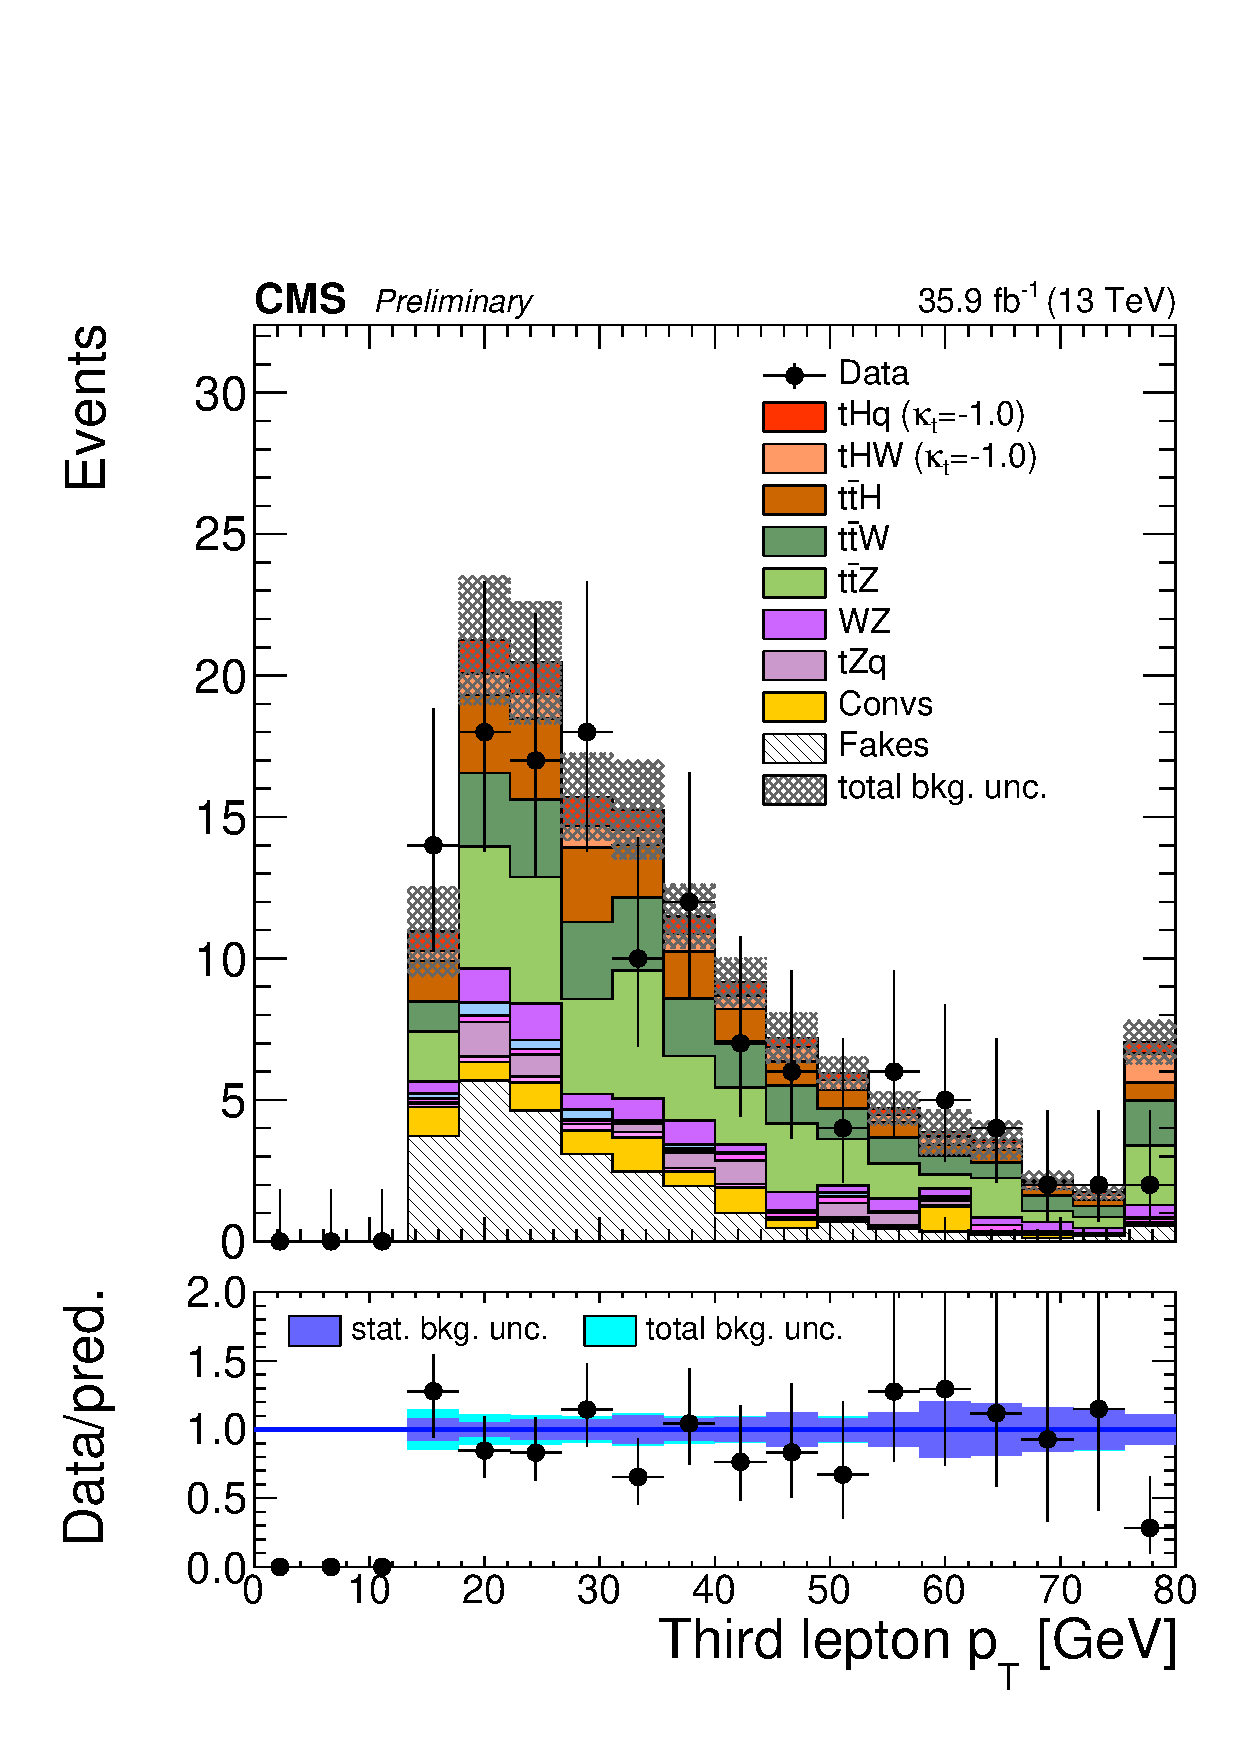
\includegraphics[width=0.22\textwidth]{figures/3lsignal/Lep3Pt.pdf} 
 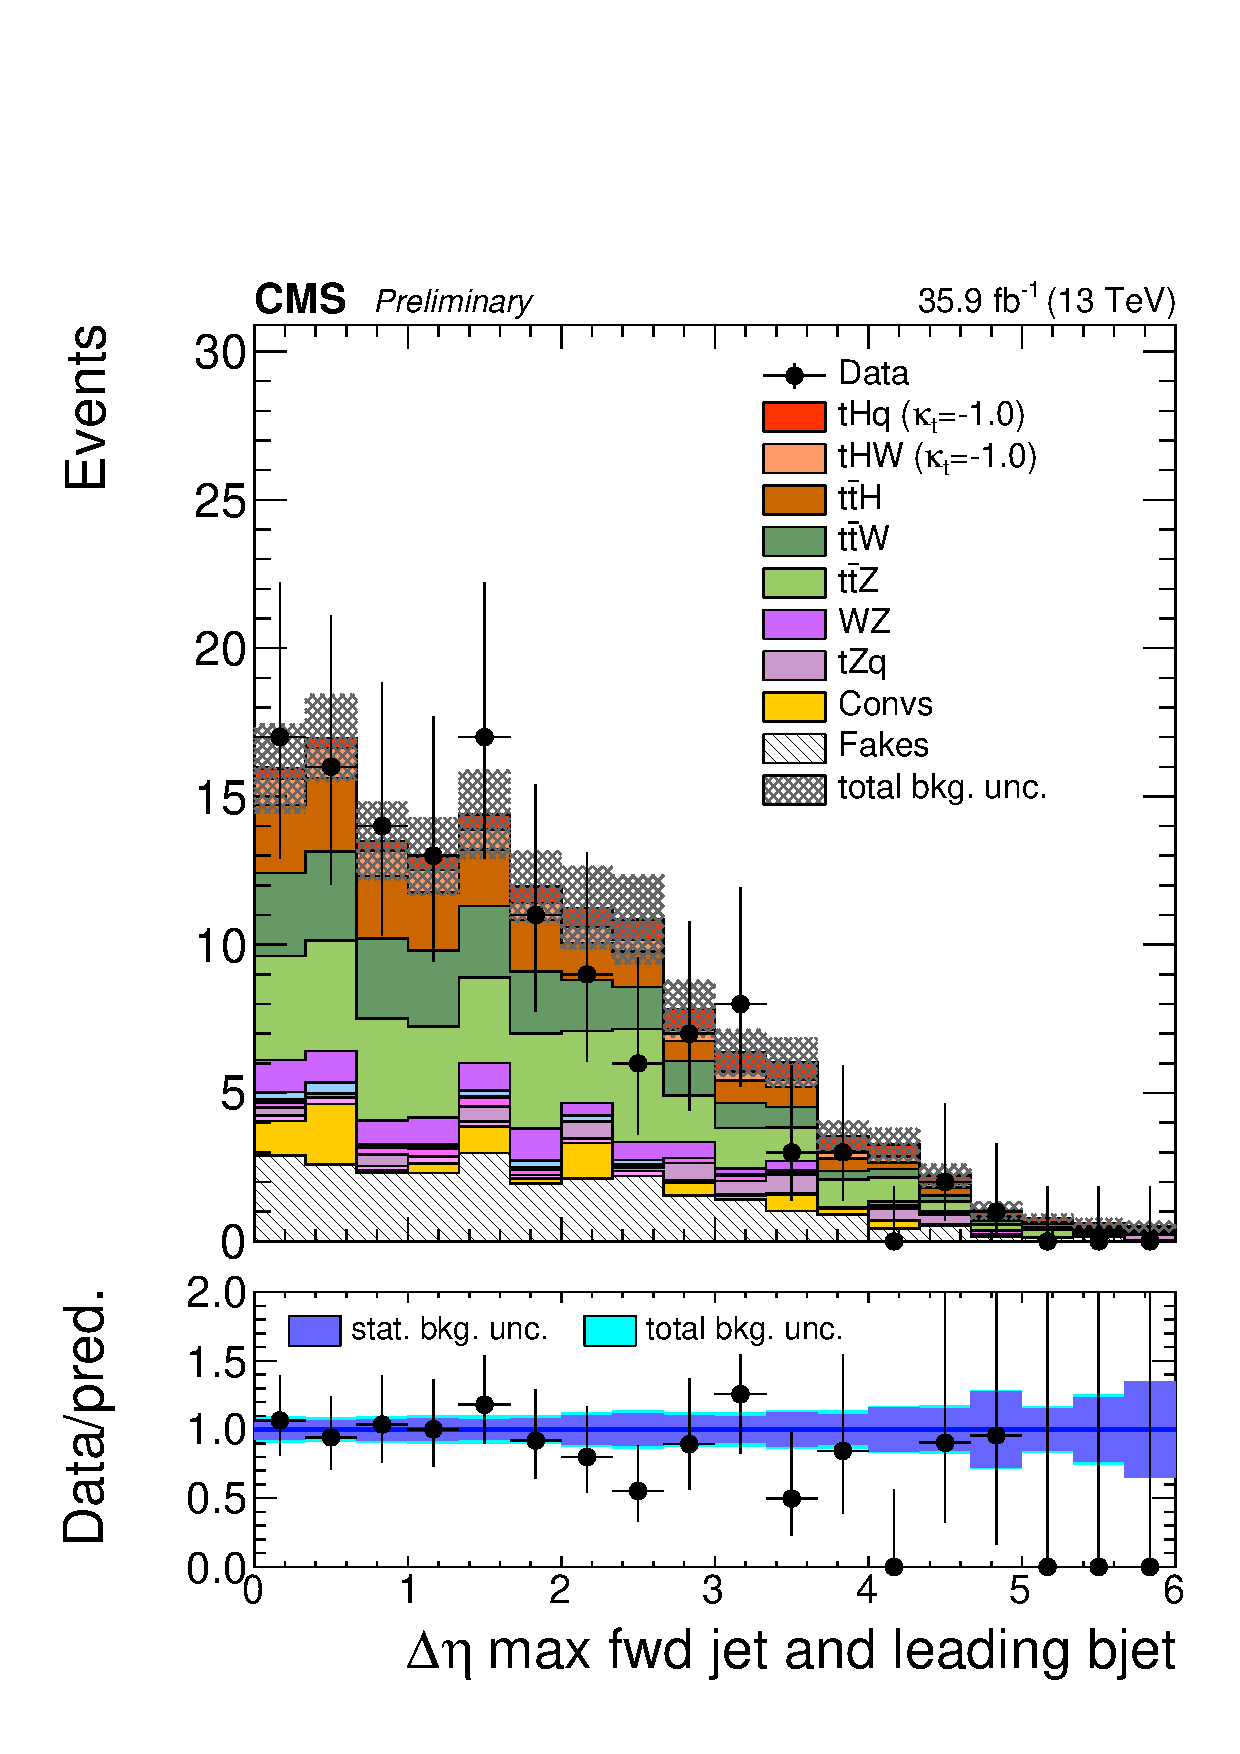
\includegraphics[width=0.22\textwidth]{figures/3lsignal/dEtaFwdJetBJet_40.pdf}
 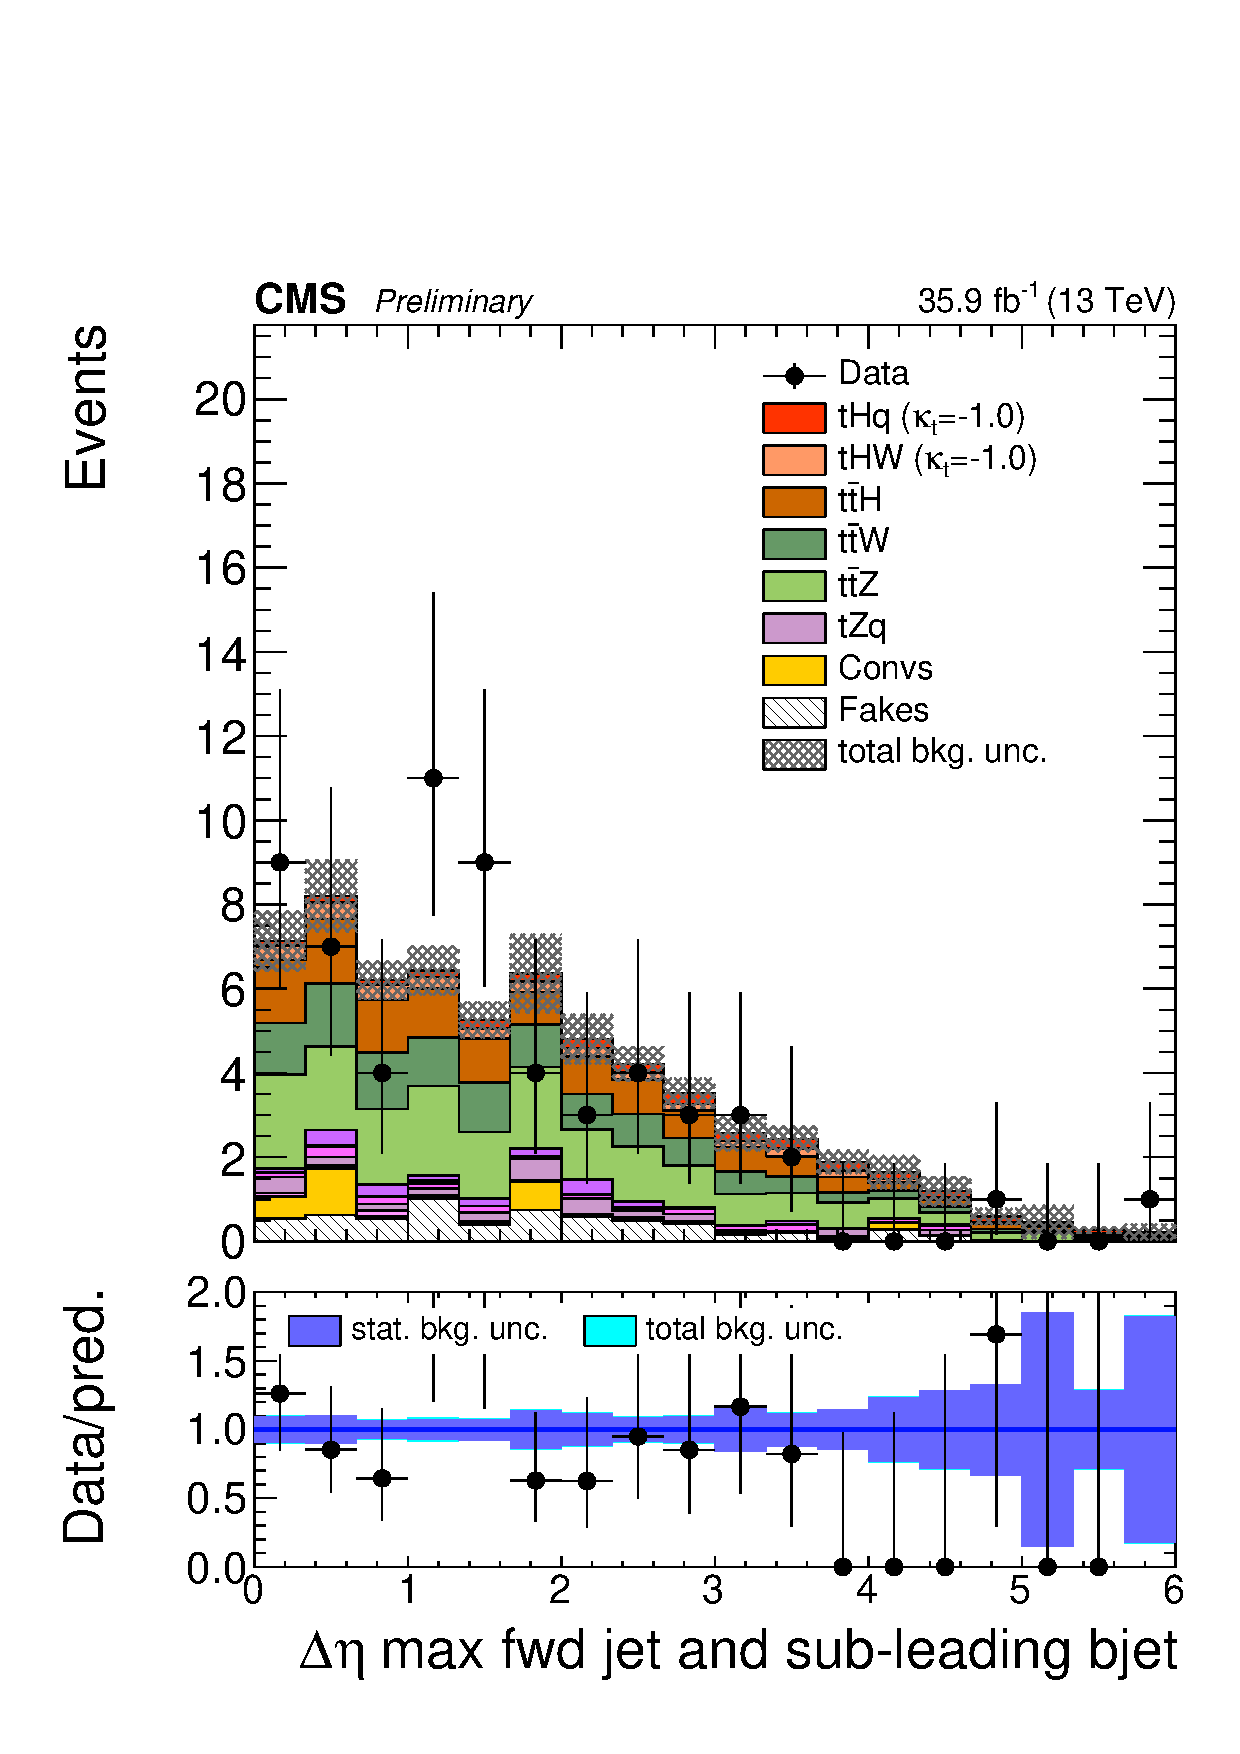
\includegraphics[width=0.22\textwidth]{figures/3lsignal/dEtaFwdJet2BJet_40.pdf}
 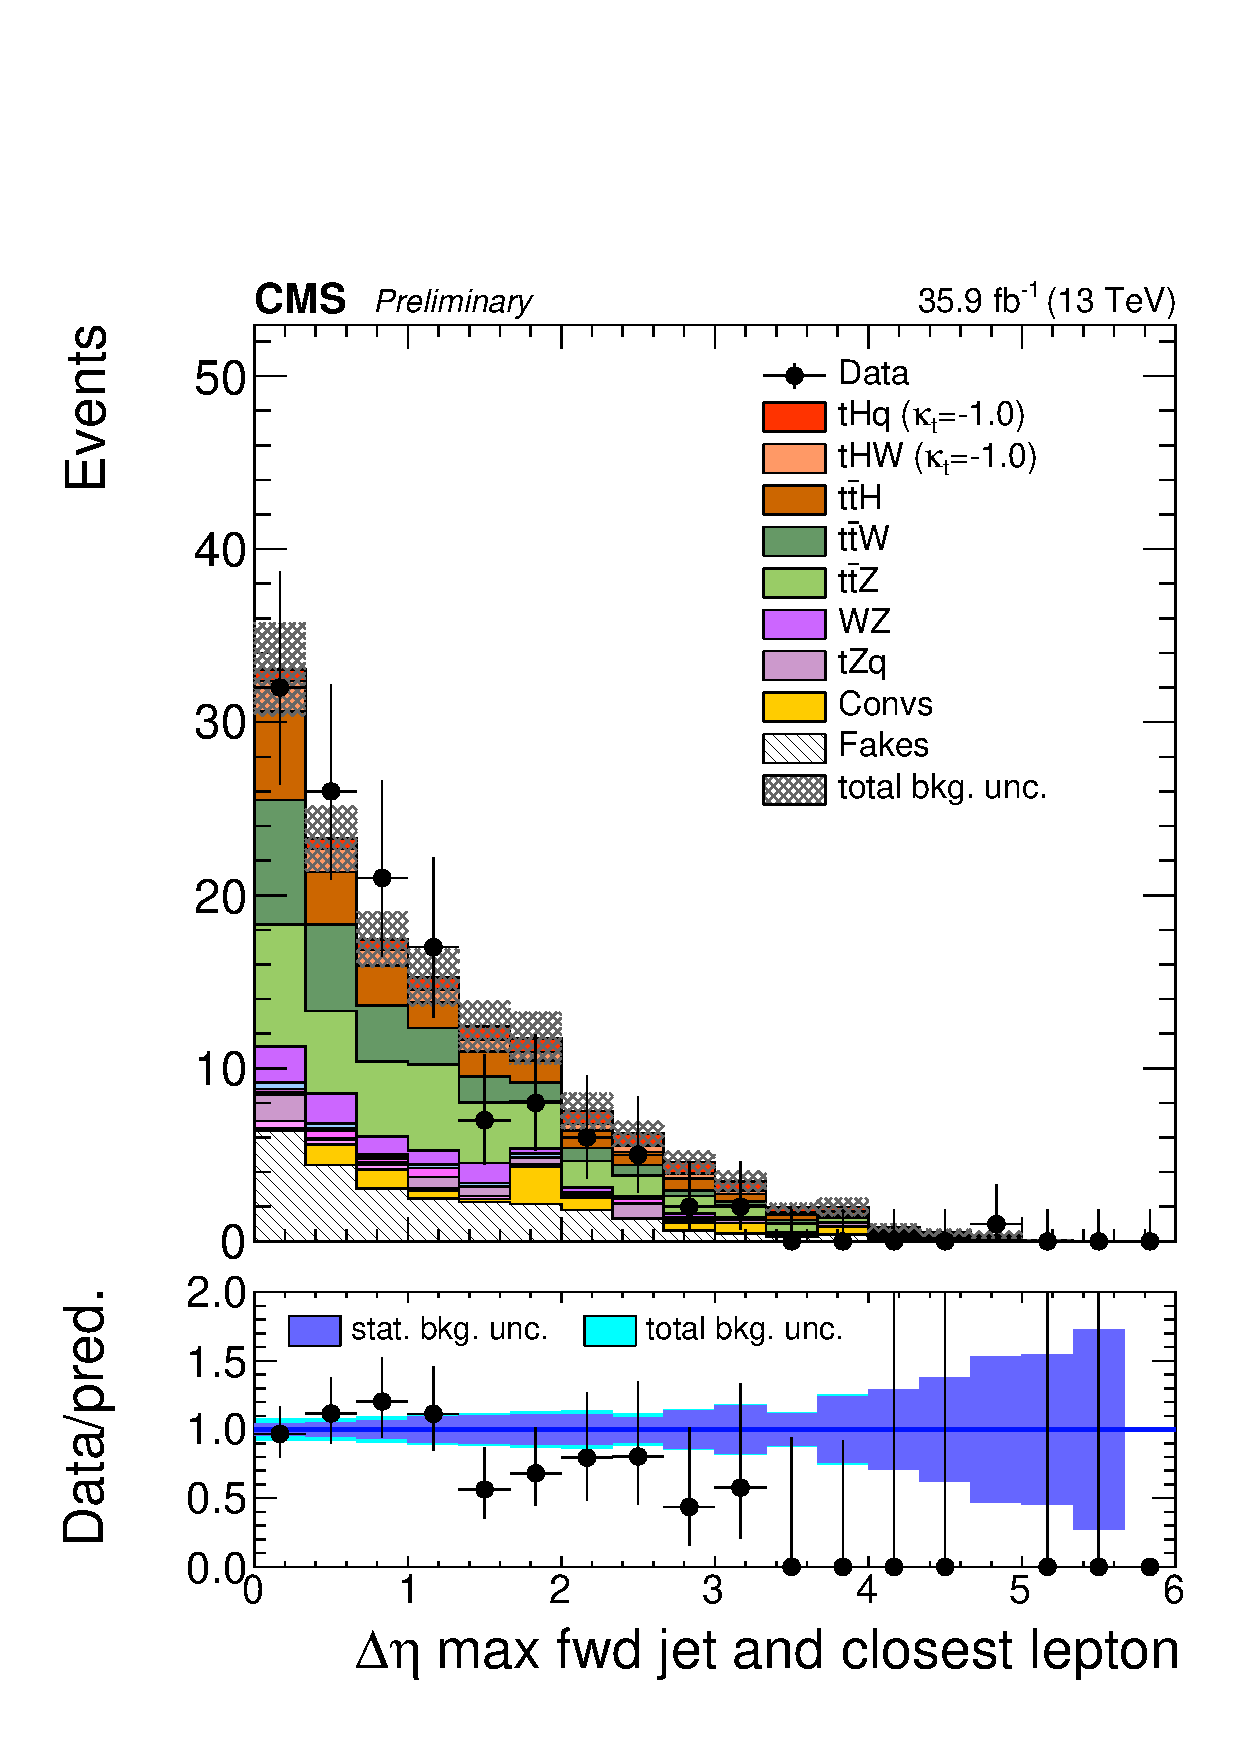
\includegraphics[width=0.22\textwidth]{figures/3lsignal/dEtaFwdJetClosestLep_40.pdf} \\
 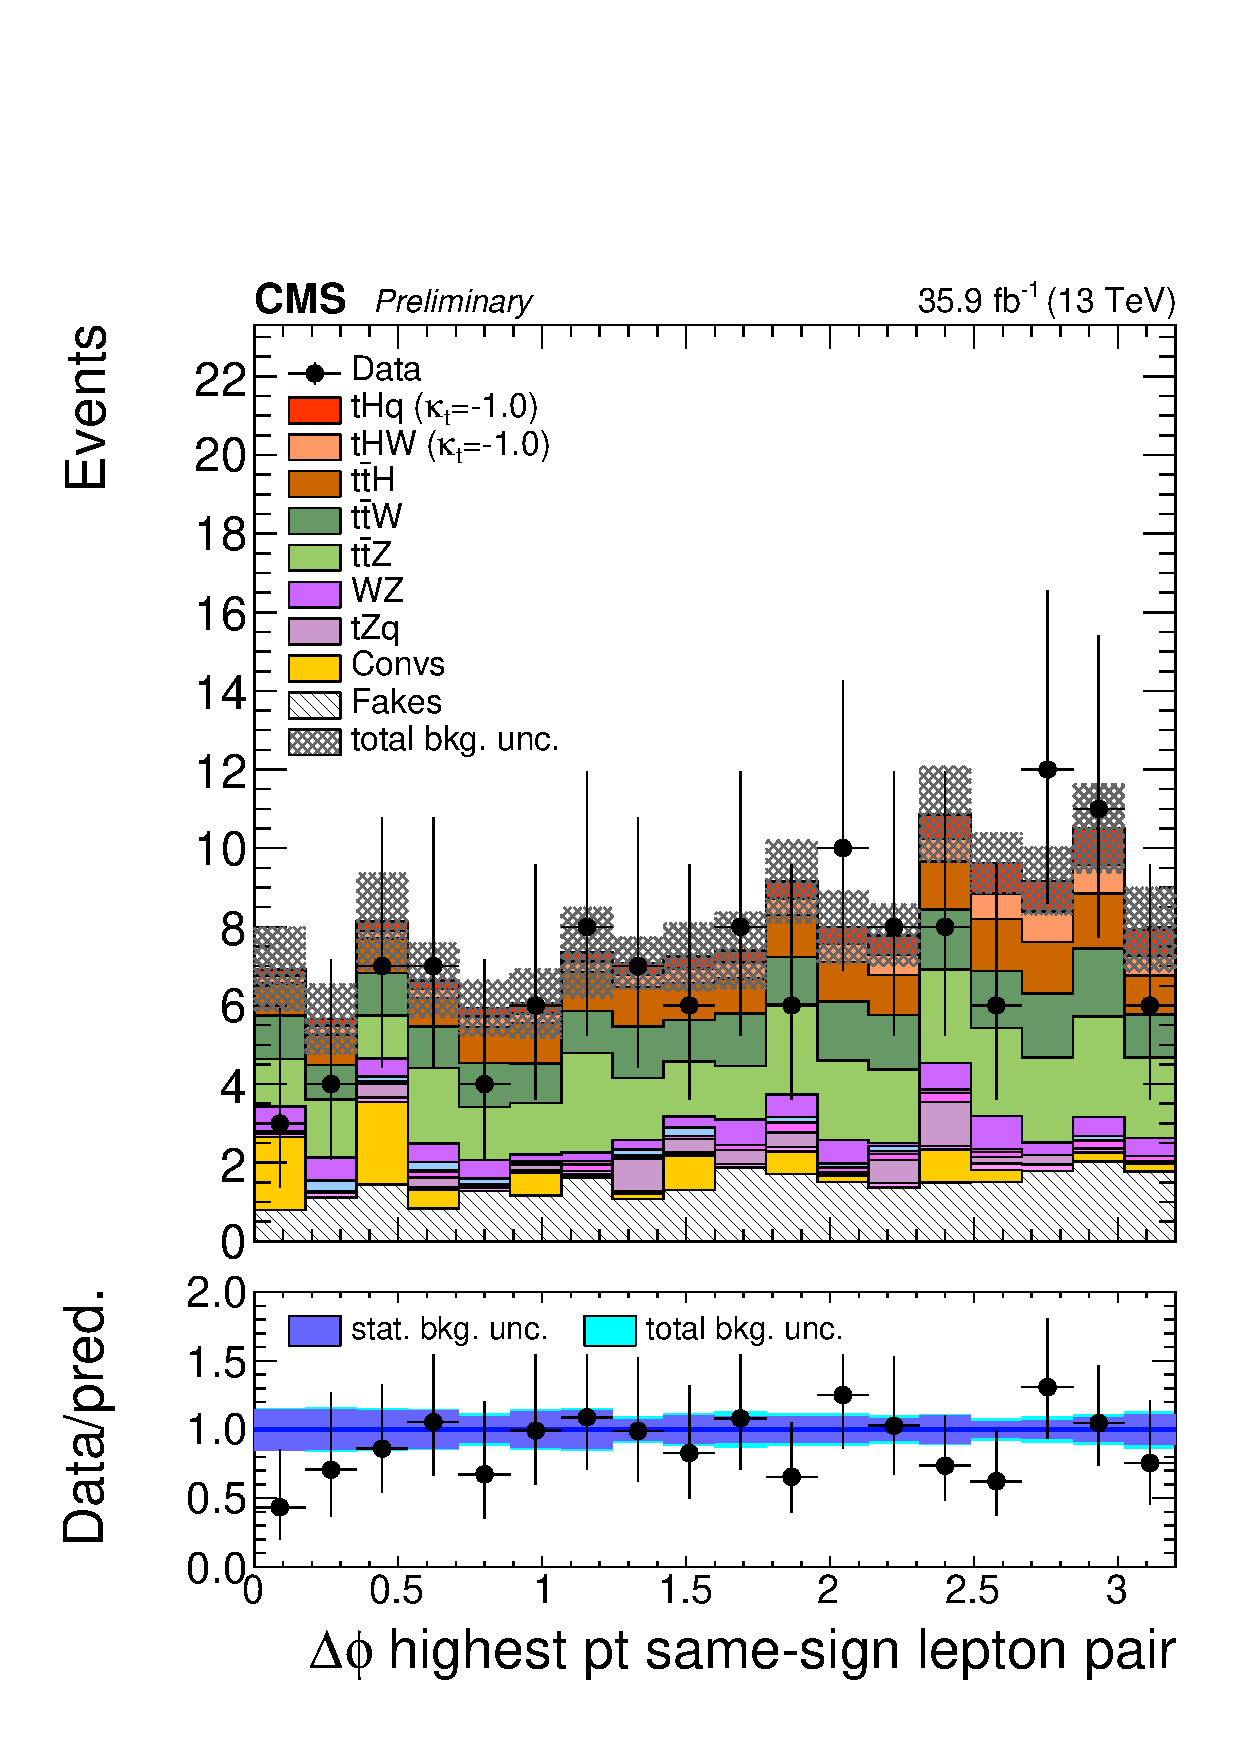
\includegraphics[width=0.22\textwidth]{figures/3lsignal/dPhiHighestPtSSPair.pdf}
 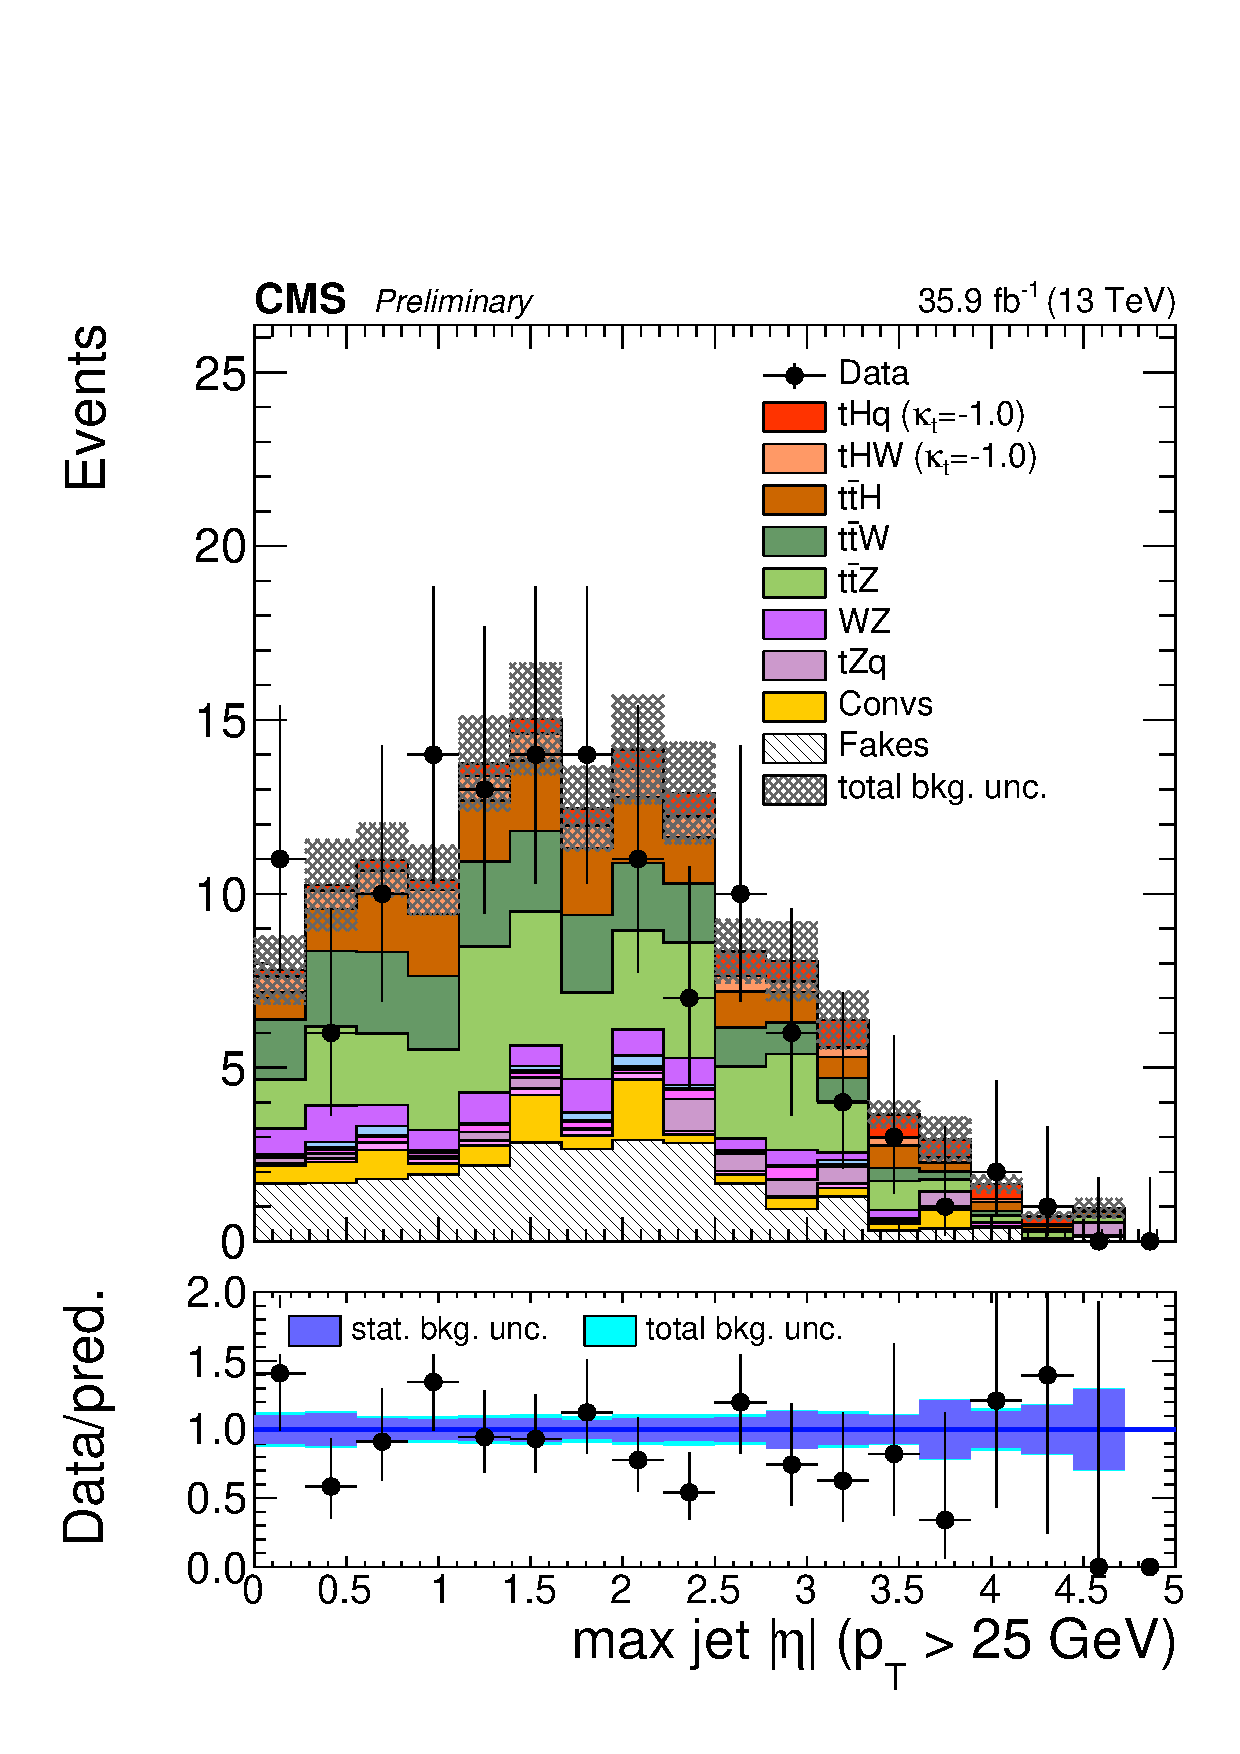
\includegraphics[width=0.22\textwidth]{figures/3lsignal/maxEtaJet25_40.pdf}
 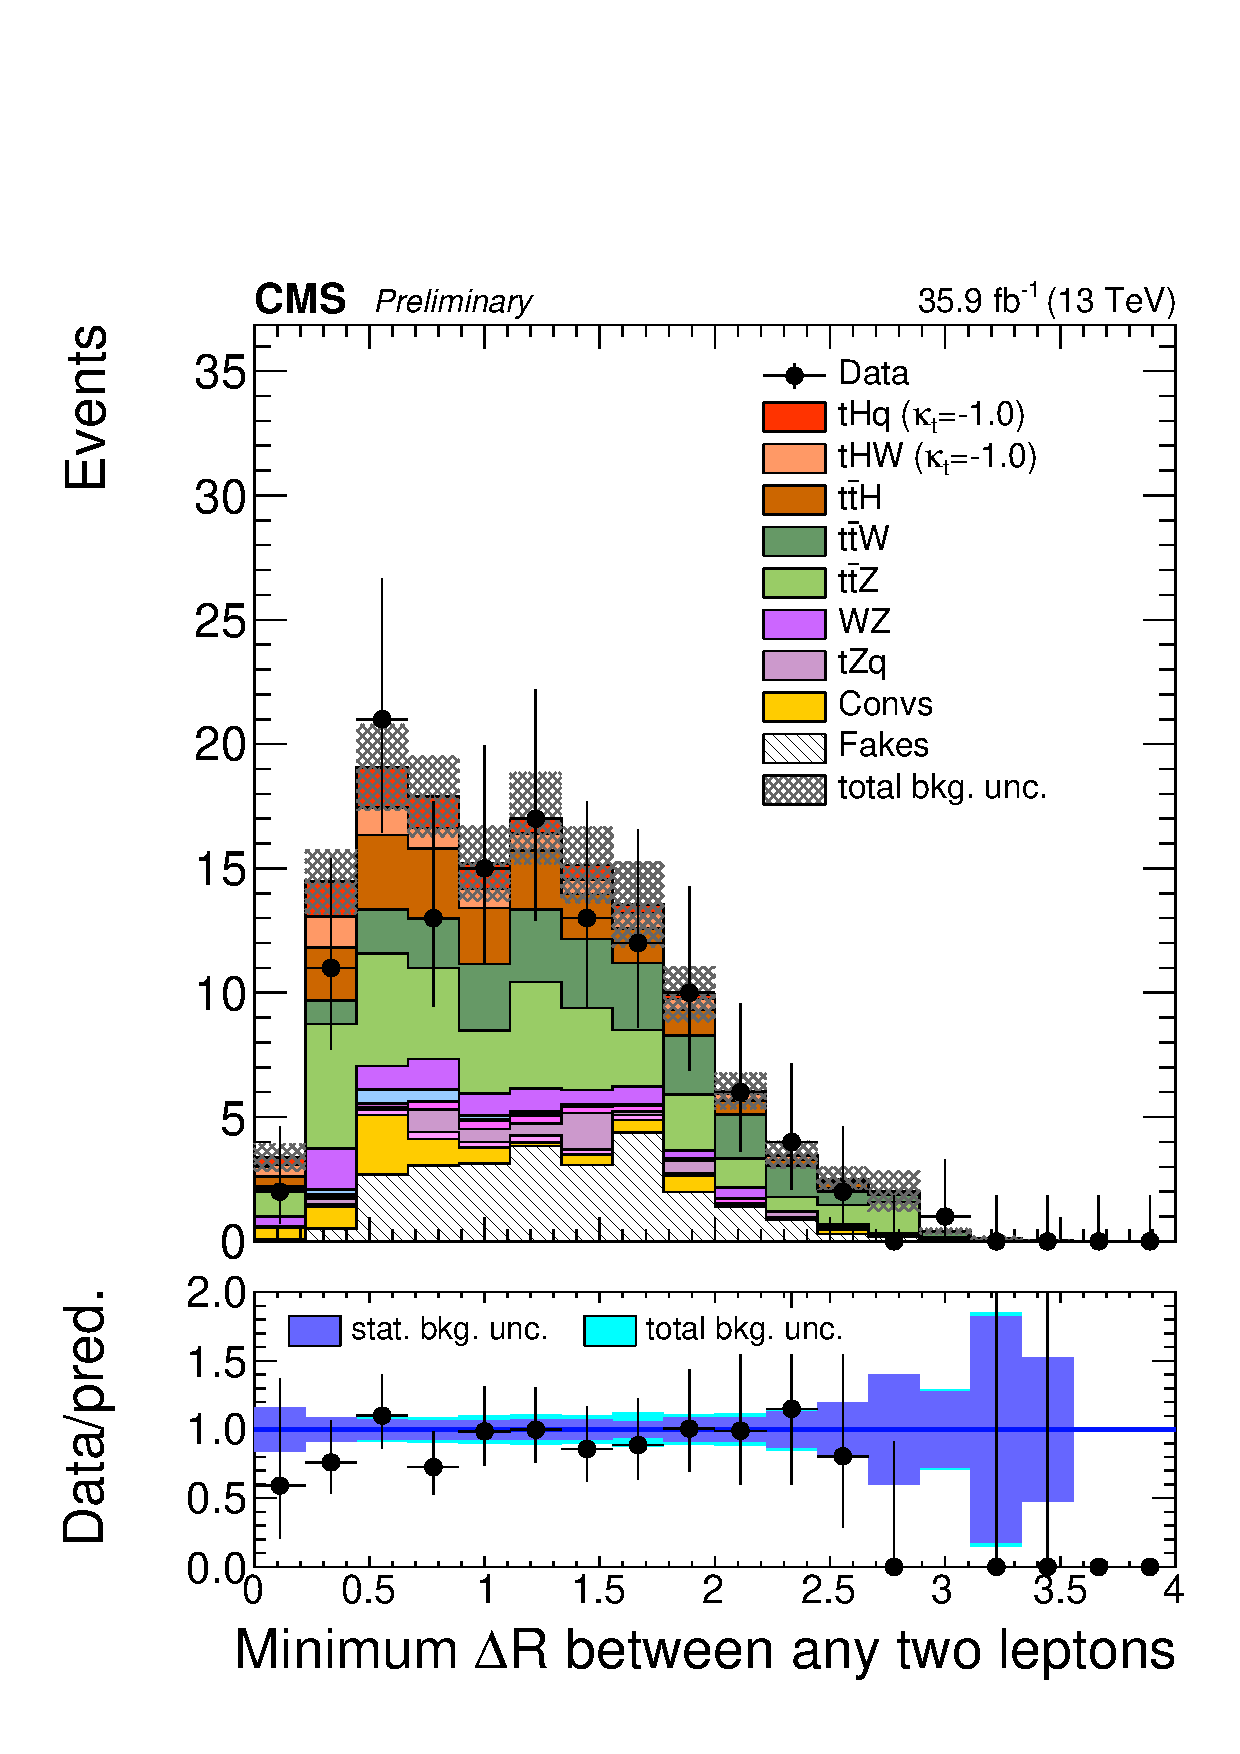
\includegraphics[width=0.22\textwidth]{figures/3lsignal/minDRll.pdf}
 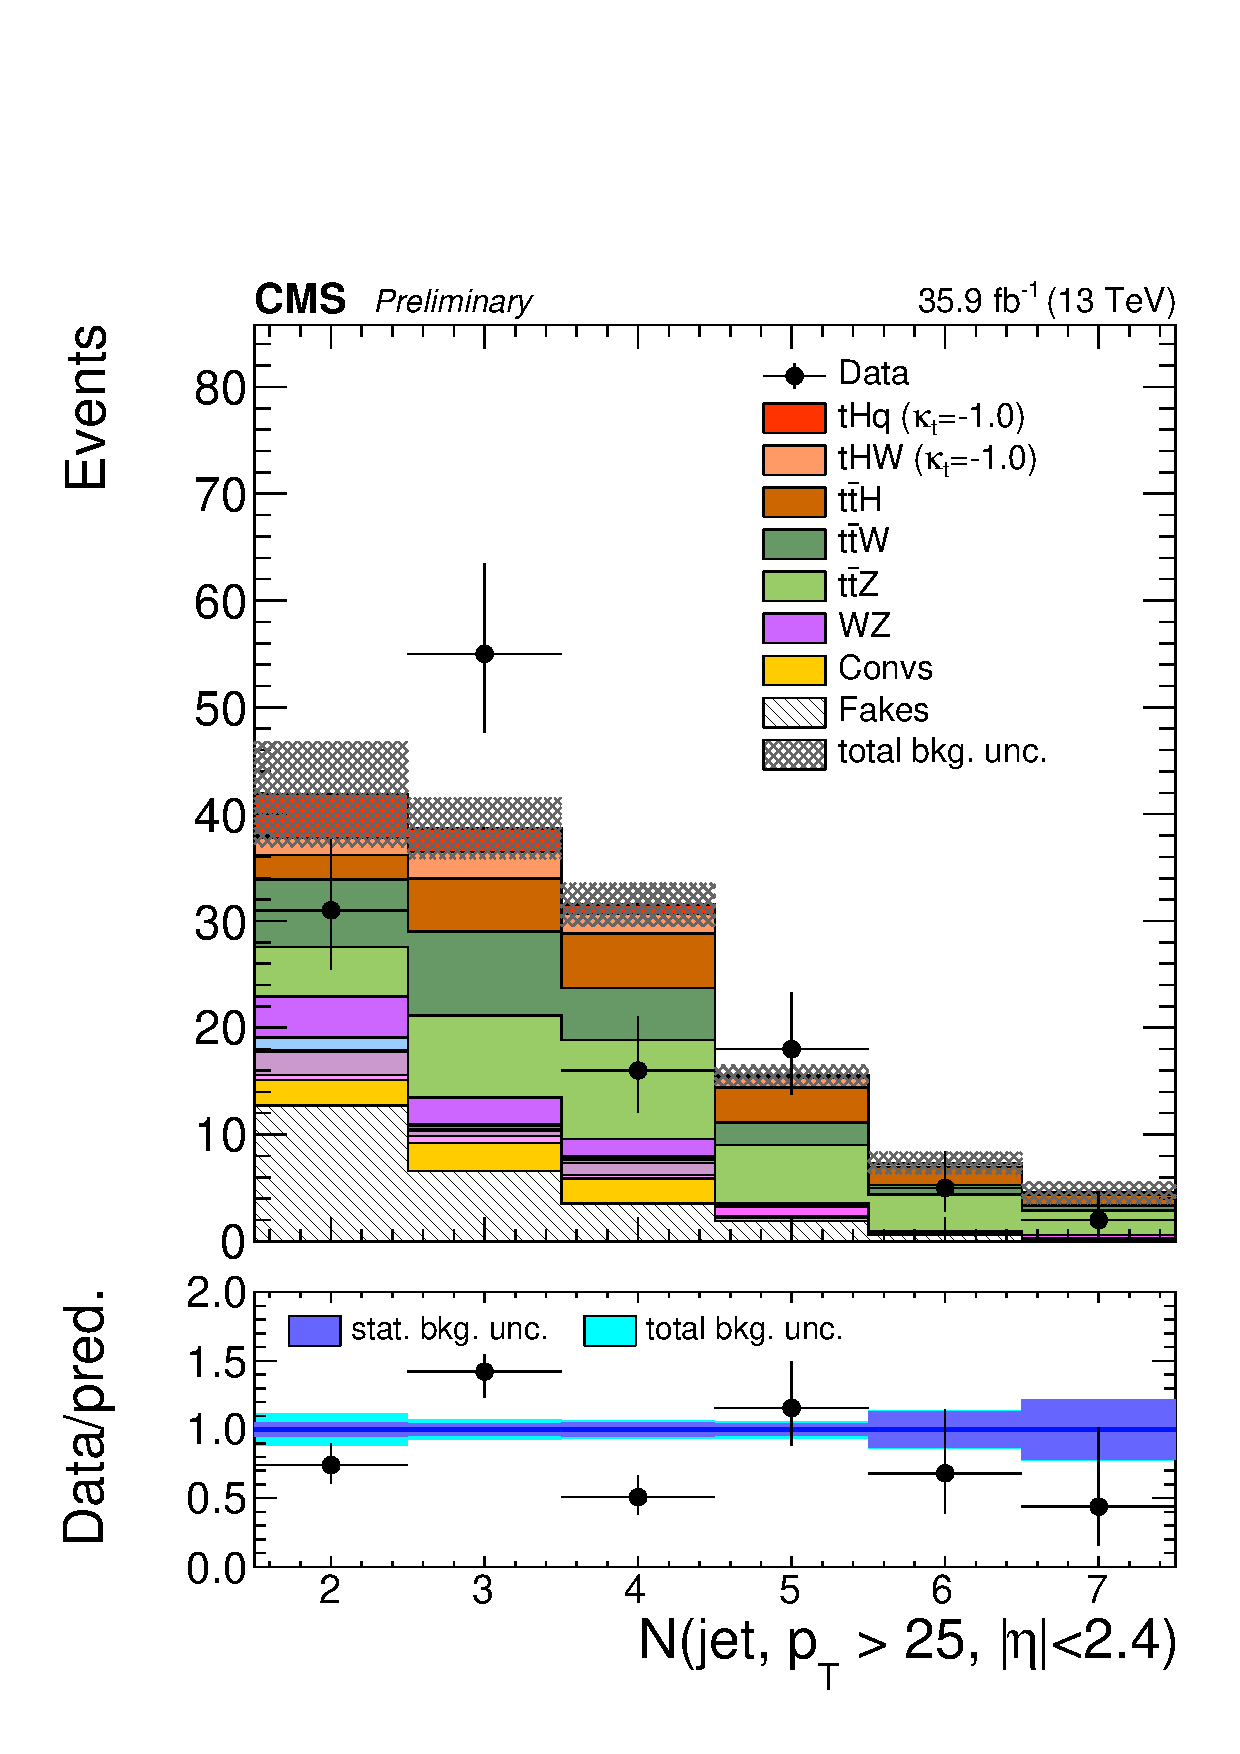
\includegraphics[width=0.22\textwidth]{figures/3lsignal/nJet25.pdf} \\
 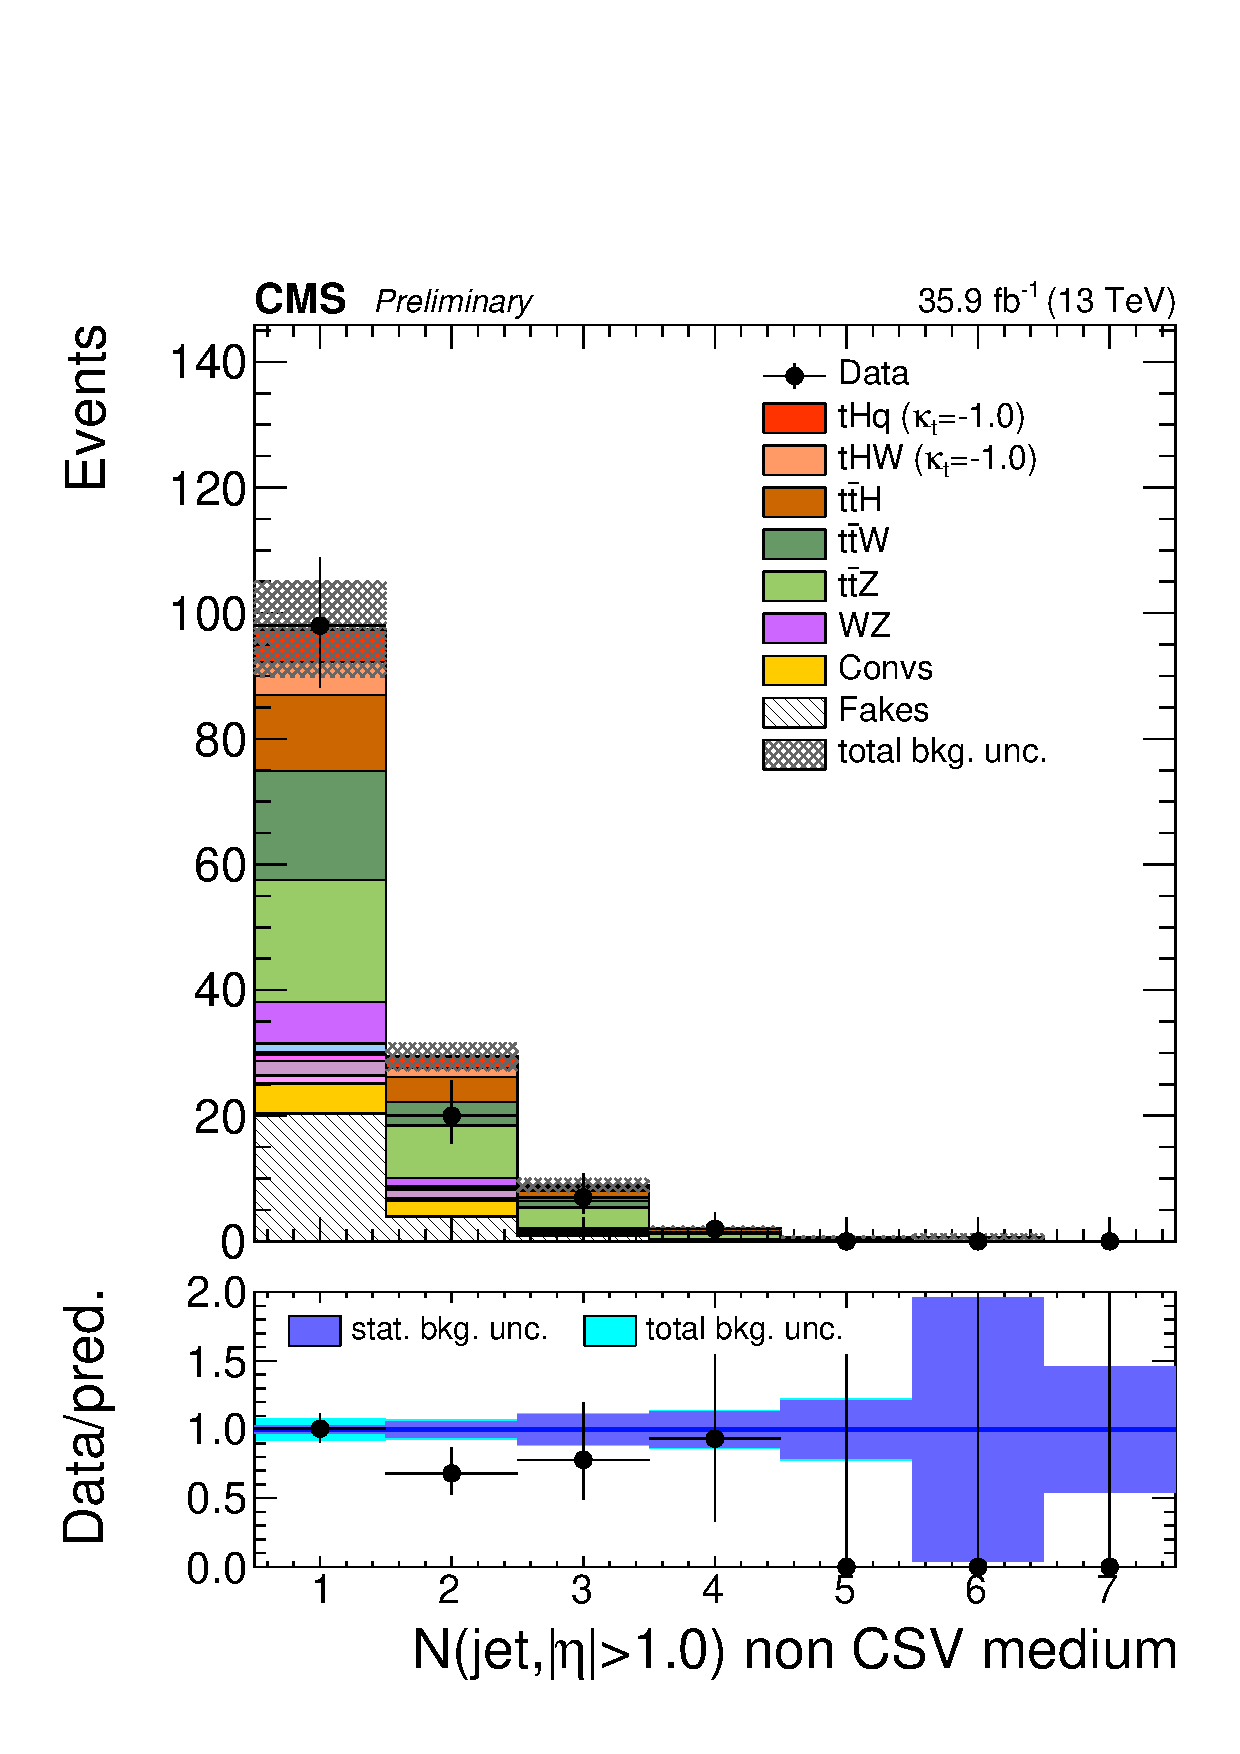
\includegraphics[width=0.22\textwidth]{figures/3lsignal/nJetEta1_40.pdf}
 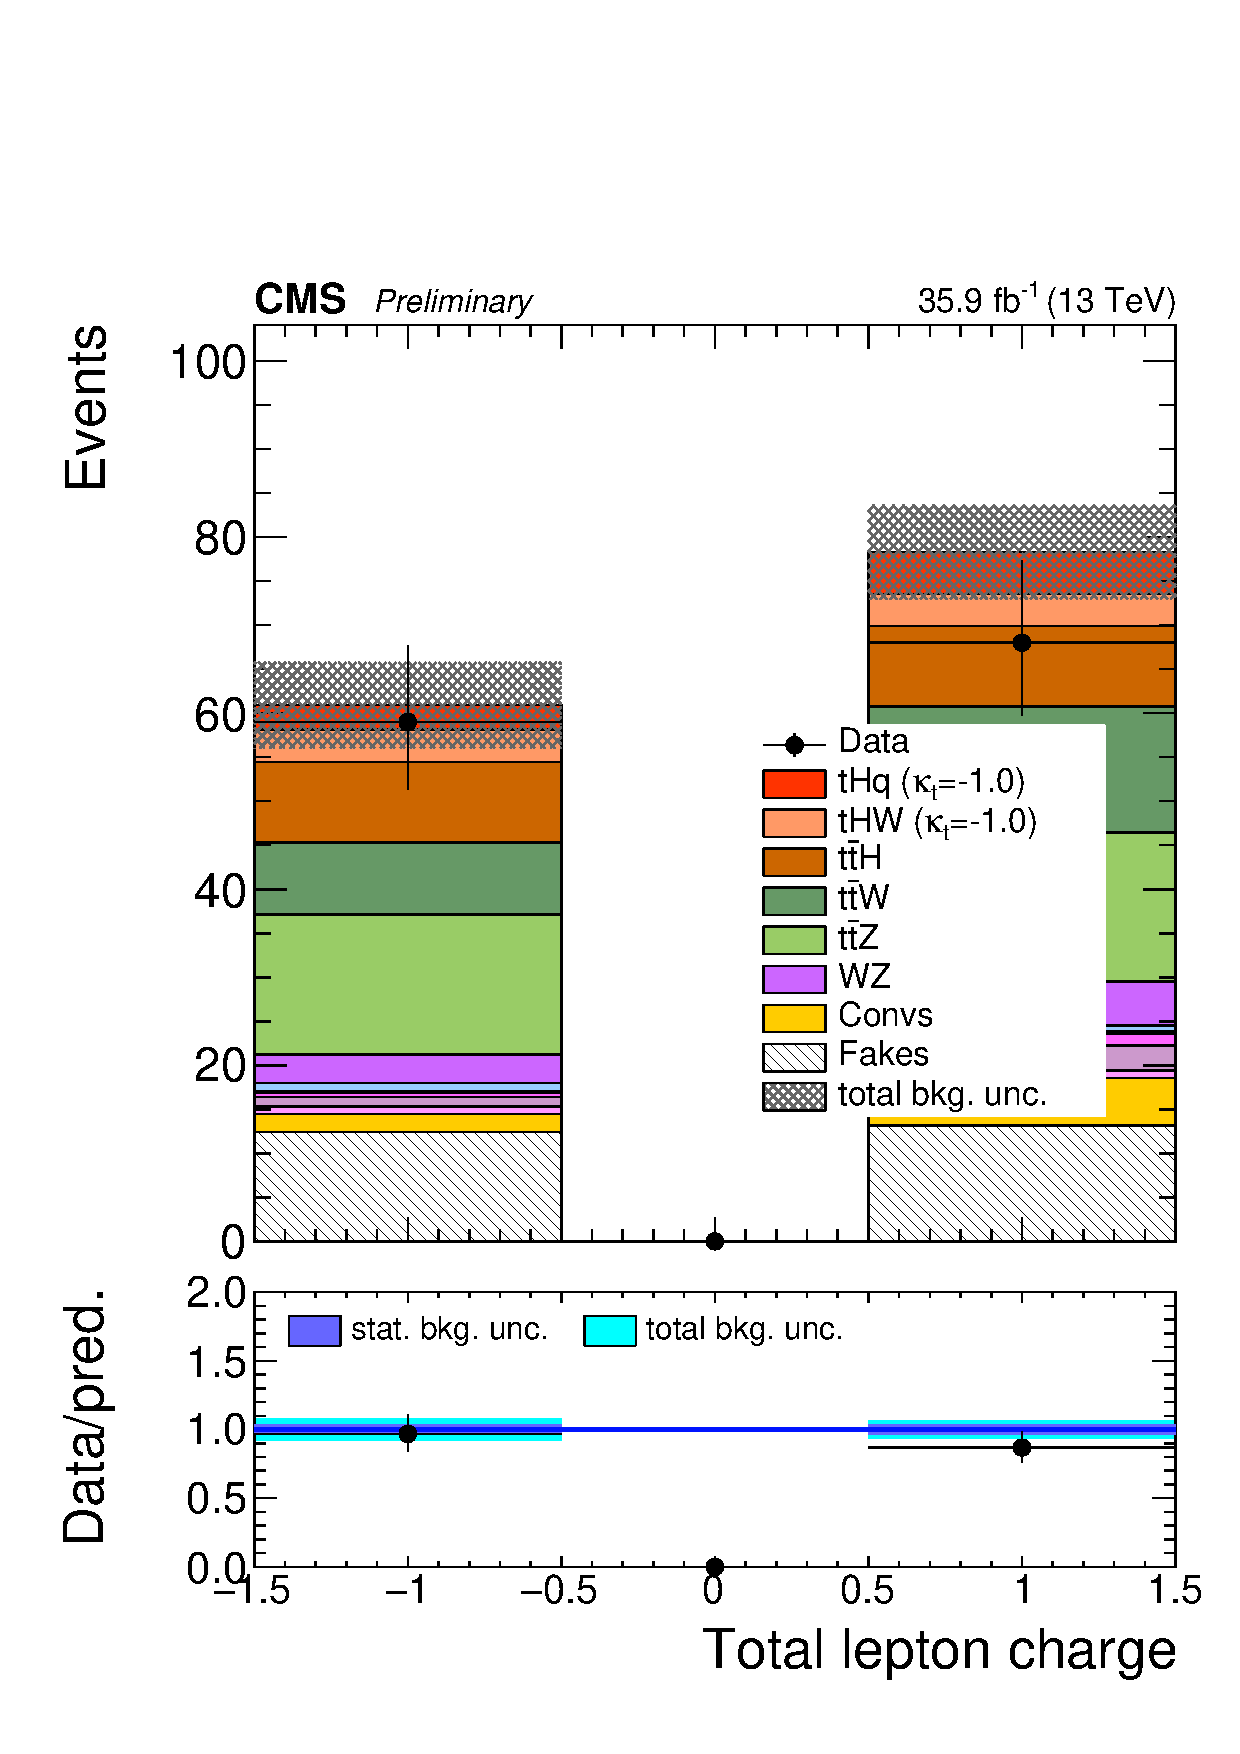
\includegraphics[width=0.22\textwidth]{figures/3lsignal/totCharge.pdf}
\caption{Distributions of input variables to the BDT for signal discrimination, three lepton channel, normalized to their cross section and to 35.9\fbinv.} 
\label{fig:input_vars_3l_xsec}
\end{figure}    

\begin{figure} [!h]
  \centering
  \includegraphics[width=0.22\textwidth]{figures/signalregion_2lss/mumu/Lep2Pt.pdf}
  \includegraphics[width=0.22\textwidth]{figures/signalregion_2lss/mumu/dEtaFwdJetBJet_40.pdf}
  \includegraphics[width=0.22\textwidth]{figures/signalregion_2lss/mumu/dEtaFwdJet2BJet_40.pdf}
  \includegraphics[width=0.22\textwidth]{figures/signalregion_2lss/mumu/dEtaFwdJetClosestLep_40.pdf} \\
  \includegraphics[width=0.22\textwidth]{figures/signalregion_2lss/mumu/dPhiHighestPtSSPair.pdf}
  \includegraphics[width=0.22\textwidth]{figures/signalregion_2lss/mumu/maxEtaJet25_40.pdf}
  \includegraphics[width=0.22\textwidth]{figures/signalregion_2lss/mumu/minDRll.pdf} 
  \includegraphics[width=0.22\textwidth]{figures/signalregion_2lss/mumu/nJet25.pdf} \\
  \includegraphics[width=0.22\textwidth]{figures/signalregion_2lss/mumu/nJetEta1_40.pdf}
  \includegraphics[width=0.22\textwidth]{figures/signalregion_2lss/mumu/totCharge.pdf}
\caption{Distributions of input variables to the BDT for signal discrimination, in \mumu\ channel, normalized to their cross section and to 35.9\fbinv.}
\label{fig:input_vars_2lss_xsec_mumu}
\end{figure}

\begin{figure} [!h]
  \centering
  \includegraphics[width=0.22\textwidth]{figures/signalregion_2lss/emu/Lep2Pt.pdf}
  \includegraphics[width=0.22\textwidth]{figures/signalregion_2lss/emu/dEtaFwdJetBJet_40.pdf}
  \includegraphics[width=0.22\textwidth]{figures/signalregion_2lss/emu/dEtaFwdJet2BJet_40.pdf}
  \includegraphics[width=0.22\textwidth]{figures/signalregion_2lss/emu/dEtaFwdJetClosestLep_40.pdf} \\
  \includegraphics[width=0.22\textwidth]{figures/signalregion_2lss/emu/dPhiHighestPtSSPair.pdf}
  \includegraphics[width=0.22\textwidth]{figures/signalregion_2lss/emu/maxEtaJet25_40.pdf}
  \includegraphics[width=0.22\textwidth]{figures/signalregion_2lss/emu/minDRll.pdf} 
  \includegraphics[width=0.22\textwidth]{figures/signalregion_2lss/emu/nJet25.pdf} \\
  \includegraphics[width=0.22\textwidth]{figures/signalregion_2lss/emu/nJetEta1_40.pdf}
  \includegraphics[width=0.22\textwidth]{figures/signalregion_2lss/emu/totCharge.pdf}
\caption{Distributions of input variables to the BDT for signal discrimination, in $e^{\pm}\mu^{\pm}$ channel, normalized to their cross section and to 35.9\fbinv.}
\label{fig:input_vars_2lss_xsec_emu}
\end{figure}

\begin{figure} [!h]
  \centering
  \includegraphics[width=0.22\textwidth]{figures/signalregion_2lss/ee/Lep2Pt.pdf}
  \includegraphics[width=0.22\textwidth]{figures/signalregion_2lss/ee/dEtaFwdJetBJet_40.pdf}
  \includegraphics[width=0.22\textwidth]{figures/signalregion_2lss/ee/dEtaFwdJet2BJet_40.pdf}
  \includegraphics[width=0.22\textwidth]{figures/signalregion_2lss/ee/dEtaFwdJetClosestLep_40.pdf} \\
  \includegraphics[width=0.22\textwidth]{figures/signalregion_2lss/ee/dPhiHighestPtSSPair.pdf}
  \includegraphics[width=0.22\textwidth]{figures/signalregion_2lss/ee/maxEtaJet25_40.pdf}
  \includegraphics[width=0.22\textwidth]{figures/signalregion_2lss/ee/minDRll.pdf} 
  \includegraphics[width=0.22\textwidth]{figures/signalregion_2lss/ee/nJet25.pdf} \\
  \includegraphics[width=0.22\textwidth]{figures/signalregion_2lss/ee/nJetEta1_40.pdf}
  \includegraphics[width=0.22\textwidth]{figures/signalregion_2lss/ee/totCharge.pdf}
\caption{Distributions of input variables to the BDT for signal discrimination, in $\Pe^{\pm}\Pe^{\pm}$ channel, normalized to their cross section and to 35.9\fbinv.}
\label{fig:input_vars_2lss_xsec_ee}
\end{figure}


\clearpage

\section{Signal discrimination}
\label{sec:sigdisc}
The \tHq\ signal is separated from the main backgrounds using a boosted decision tree (BDT) classifier, trained on simulated signal and background events.
A set of discriminating variables are given as input to the BDT which produces a output distribution maximizing the discrimination power.
Table~\ref{tab:bdtinputs} lists the input variables used while Figures~\ref{fig:input_vars_3l} and~\ref{fig:input_vars_2lss} show their distributions for the relevant signal and background samples, for the three lepton and same-sign dilepton channels, respectively.
The same or equivalent input variables are found to be performing well for both three lepton and same-sign dilepton channels.

Two BDT classifiers are trained for the two main backgrounds expected in the analysis: events with prompt leptons from \ttW\ and \ttZ\ (also referred to as \ttV), and events with non-prompt leptons from \ttbar.
The datasets used in the training are the \tHq\ signal (see Tab.~\ref{tab:sigsamples}), and LO \MADGRAPH\ samples of \ttW\ and \ttZ, in an admixture proportional to their respective cross sections (see Tab.~\ref{tab:ttvlo_samples}).

\begin{table}[h!]
\centering
\begin{tabular}{lp{10cm}}
Variable name        & Description\\ \hline
nJet25               & Number of jets with $\pt>25\GeV$, $|\eta|<2.4$\\
MaxEtaJet25          & Maximum $|\eta|$ of any (non-CSV-loose) jet with $\pt>25\GeV$\\
% nBJetLoose25         & Number of jets with $\pt>25\GeV$, CSV loose\\
totCharge            & Sum of lepton charges \\
nJetEta1             & Number of jets with $|\eta|>1.0$, non-CSV-loose\\
detaFwdJetBJet       & $\Delta \eta$ between forward light jet and hardest CSV loose jet\\
detaFwdJet2BJet      & $\Delta \eta$ between forward light jet and second hardest CSV loose jet (defaults to -1 in events with only one CSV loose jet) \\
detaFwdJetClosestLep & $\Delta \eta$ between forward light jet and closest lepton\\
dphiHighestPtSSPair  & $\Delta \phi$ of highest \pt\ same-sign lepton pair\\
minDRll              & minimum $\Delta R$ between any two leptons\\
Lep3Pt/Lep2Pt        & \pt\ of the $3^{rd}$ lepton ($2^{nd}$ for ss2l)\\ \hline
\end{tabular}
\caption{MVA input discriminating variables}
\label{tab:bdtinputs}
\end{table}


\begin{figure} [!h]
 \centering
 \includegraphics[width=0.245\textwidth]{figures/Lep3Pt.pdf} 
 \includegraphics[width=0.245\textwidth]{figures/dEtaFwdJetBJet.pdf}
 \includegraphics[width=0.245\textwidth]{figures/dEtaFwdJet2BJet.pdf}
 \includegraphics[width=0.245\textwidth]{figures/dEtaFwdJetClosestLep.pdf} \\
 \includegraphics[width=0.245\textwidth]{figures/dPhiHighestPtSSPair.pdf}
 \includegraphics[width=0.245\textwidth]{figures/maxEtaJet25.pdf}
 \includegraphics[width=0.245\textwidth]{figures/minDRll.pdf}
 \includegraphics[width=0.245\textwidth]{figures/nJet25.pdf} \\
 \includegraphics[width=0.245\textwidth]{figures/nJetEta1.pdf}
 \includegraphics[width=0.245\textwidth]{figures/totCharge.pdf}
\caption{Distributions of input variables to the BDT for signal discrimination, three lepton channel.} 
\label{fig:input_vars_3l}
\end{figure}    

\begin{figure} [!h]
  \centering
  \includegraphics[width=0.245\textwidth]{figures/Lep2Pt_mumu.pdf} 
  \includegraphics[width=0.245\textwidth]{figures/dEtaFwdJetBJet_mumu.pdf}
  \includegraphics[width=0.245\textwidth]{figures/dEtaFwdJet2BJet_mumu.pdf}
  \includegraphics[width=0.245\textwidth]{figures/dEtaFwdJetClosestLep_mumu.pdf} \\
  \includegraphics[width=0.245\textwidth]{figures/dPhiHighestPtSSPair_mumu.pdf}
  \includegraphics[width=0.245\textwidth]{figures/maxEtaJet25_mumu.pdf}
  \includegraphics[width=0.245\textwidth]{figures/minDRll_mumu.pdf}
  \includegraphics[width=0.245\textwidth]{figures/nJet25_mumu.pdf} \\
  \includegraphics[width=0.245\textwidth]{figures/nJetEta1_mumu.pdf}
  \includegraphics[width=0.245\textwidth]{figures/totCharge_mumu.pdf}
 \caption{Distributions of input variables to the BDT for signal discrimination, two lepton same sign channel.}
\label{fig:input_vars_2lss}
\end{figure}    

The MVA analysis consist of two stages: first a ``training'' where the MVA method is trained to discriminate between simulated signal and background events, then a ``test'' stage where the trained algorithm is used to classify different events from the samples.
The sample is obtained from a pre-selection (see Tab.~\ref{tab:evsel} with pre-selection cuts).

Figures~\ref{mva_input_tt} and~\ref{mva_input_ttv} show the input variables distributions as seen by the MVA algorithm.
Note that in contrast to the distributions in Fig.~\ref{fig:input_vars_3l} only the main backgrounds (\ttbar\ from simulation, \ttV) are included.

\begin{figure} [!h]
  \centering
  \includegraphics[width=\textwidth]{figures/mva_input1_tt.pdf}
  \includegraphics[width=\textwidth]{figures/mva_input2_tt.pdf}
\caption{BDT inputs as seen by TMVA (signal, in blue, is \tHq, background, in red, is \ttbar) for the three lepton channel, discriminated against \ttbar\ (fakes) background.} 
\label{mva_input_tt}
\end{figure}

\begin{figure} [!h]
  \centering
  \includegraphics[width=\textwidth]{figures/mva_input1_ttv.pdf}
  \includegraphics[width=\textwidth]{figures/mva_input2_ttv.pdf}
\caption{BDT inputs as seen by TMVA (signal, in blue, is \tHq, background, in red, is \ttW+\ttZ) for the three lepton channel, discriminated against \ttV\ background.}                                                                                                                                                         
\label{mva_input_ttv}
\end{figure}

The input variables distributions for 2lss channel for signal against the \ttbar\ and \ttV\ are shown in Figure~\ref{mva_input_2lss_tt} and Figure~\ref{mva_input_2lss_ttv} respectively.
\begin{figure} [!h]
  \centering
  \includegraphics[width=\textwidth]{figures/6var_tt.pdf}
  \includegraphics[width=0.66\textwidth]{figures/4var_tt.pdf}
\caption{BDT inputs as seen by TMVA (signal, in blue, is \tHq, background, in red, is \ttbar) for the same sign dilepton channel, discriminated against \ttbar\ background.} 
\label{mva_input_2lss_tt}
\end{figure}

\begin{figure} [!h]
  \centering
  \includegraphics[width=\textwidth]{figures/6var_ttv.pdf}
  \includegraphics[width=0.66\textwidth]{figures/4var_ttv.pdf}
\caption{BDT inputs as seen by TMVA (signal, in blue, is \tHq, background, in red, is \ttW+\ttZ) for the same sign dilepton channel, discriminated against \ttV\ background.}
\label{mva_input_2lss_ttv}
\end{figure}

Note that splitting the training in two groups reveals that some variables show opposite behavior for the two background sources; potentially screening the discrimination power if they were to be used in a single discriminant.
For some other variables the distributions are similar in both background cases.

From table~\ref{tab:bdtinputs}, it is clear that the input variables are correlated to some extend. These correlations play an important role for some MVA methods like the Fisher discriminant method in which the first step consist of performing a linear transformation to an phase space where the correlations between variables are removed. In case a boosted decision tree (BDT) method however, correlations do not affect the performance.

Figure~\ref{mva_corr} show the linear correlation coefficients for signal and background for the two training cases (the signal values are identical by construction). As expected, strong correlations appears for variables related to the forward jet activity. Same trend is seen in case of the same sign dilepton channel in Figure~\ref{mva_corr_2lss}.

\begin{figure} [!h]
  \centering
   \includegraphics[width=0.32\textwidth]{figures/corr_signal.pdf}
   \includegraphics[width=0.32\textwidth]{figures/corr_tt.pdf}
   \includegraphics[width=0.32\textwidth]{figures/corr_ttv.pdf}

\caption{ Signal (left), \ttbar\ background (middle), and \ttV\ background (right.) correlation matrices for the input variables in the TMVA analysis for the three lepton channel.}
\label{mva_corr}
\end{figure}

\begin{figure} [!h]
  \centering
  \includegraphics[width=0.32\textwidth]{figures/sig_corr_tt_2lss.pdf}
  \includegraphics[width=0.32\textwidth]{figures/bkg_corr_tt_2lss.pdf}
  \includegraphics[width=0.32\textwidth]{figures/bkg_corr_ttv_2lss.pdf}
\caption{Signal and Background correlation matrices for the input variables in the TMVA analysis for the same sign dilepton channel, for the signal (left), \ttbar\ background (middle), and \ttV\ background (right.)}
\label{mva_corr_2lss}
\end{figure}

\subsection{Classifiers response}
Several MVA algorithms were evaluated to determine the most appropriate method for this analysis.
The plots in Fig.~\ref{roc} (top) show the background rejection as a function of the signal efficiency for \ttbar\ and \ttV\ trainings (ROC curves) for the different algorithms that were evaluated.

\begin{figure} [!h]
  \centering
   \includegraphics[width=0.4\textwidth]{figures/roc_ttv_3l_multimva.pdf}
   \includegraphics[width=0.4\textwidth]{figures/roc_tt_3l_multimva.pdf} \\
   \includegraphics[width=0.4\textwidth]{figures/bdt_response_ttv_3l.pdf}
   \includegraphics[width=0.4\textwidth]{figures/bdt_response_tt_3l.pdf}
\caption{Top: background rejection vs signal efficiency (ROC curves) for various MVA classifiers (top) in the three lepton channel against \ttV\ (left) and \ttbar\ (right). Bottom: classifier output distributions for the gradient boosted decision trees, for training against \ttV\ (left) and against \ttbar\ (right).}
\label{roc}
\end{figure} 

\begin{figure} [!h]
  \centering
   \includegraphics[width=0.4\textwidth]{figures/roc_ttv_2lss.pdf}
   \includegraphics[width=0.4\textwidth]{figures/roc_tt_2lss.pdf} \\
   \includegraphics[width=0.4\textwidth]{figures/bdt_output_ttv_2lss.pdf}
   \includegraphics[width=0.4\textwidth]{figures/bdt_output_tt_2lss.pdf}
\caption{Top: background rejection vs signal efficiency (ROC curve) in the same sign dilepton channel for a single discriminator: BDTG, against \ttV\ (left) and \ttbar\ (right). Bottom: classifier output distribution, for training against \ttV\ (left) and against \ttbar\ (right).}
\label{output_2lss}
\end{figure}

In both cases the gradient boosted decision tree (``BDTA\_GRAD'') classifier offers the best results, followed by an adaptive BDT classifier (``BDTA''). 
The BDTA\_GRAD classifier output distributions for signal and backgrounds are shown on the bottom of Fig.~\ref{roc}.
As expected, a good discrimination power is obtained using default discriminator parameter values, with minimal overtraining.
TMVA provides a ranking of the input variables by their importance in the classification process, shown in Tab.~\ref{ranking}.

\begin{table}[h!]
\centering
\footnotesize
\begin{tabular}{lllll}
      &\multicolumn{2}{c}{ttbar training}             & \multicolumn{2}{c}{ttV training}\\\hline
Rank  & Variable             & Importance  & Variable             & Importance \\ \hline
    1 & minDRll              & 1.329e-01   & dEtaFwdJetBJet       & 1.264e-01\\
    2 & dEtaFwdJetClosestLep & 1.294e-01   & Lep3Pt               & 1.224e-01\\
    3 & dEtaFwdJetBJet       & 1.209e-01   & maxEtaJet25          & 1.221e-01\\
    4 & dPhiHighestPtSSPair  & 1.192e-01   & dEtaFwdJet2BJet      & 1.204e-01\\
    5 & Lep3Pt               & 1.158e-01   & dEtaFwdJetClosestLep & 1.177e-01\\
    6 & maxEtaJet25          & 1.121e-01   & minDRll              & 1.143e-01\\
    7 & dEtaFwdJet2BJet      & 9.363e-02   & dPhiHighestPtSSPair  & 9.777e-02\\
    8 & nJetEta1             & 6.730e-02   & nJet25\_Recl         & 9.034e-02\\
    9 & nJet25\_Recl         & 6.178e-02   & nJetEta1             & 4.749e-02\\
   10 & lepCharge            & 4.701e-02   & lepCharge            & 4.116e-02\\\hline

\end{tabular}
\caption{TMVA input variables ranking for BDTA\_GRAD method for the trainings in the three lepton channel. For both trainings the rankings show almost the same 5 variables in the first places.}

\label{ranking}
\end{table}

\begin{table}[h!]
\centering
\footnotesize
\begin{tabular}{lllll}
      &\multicolumn{2}{c}{ttbar training}             & \multicolumn{2}{c}{ttV training}\\\hline
Rank  & Variable             & Importance  & Variable             & Importance \\ \hline
    1 & dEtaFwdJetClosestLep & 1.394e-01   & maxEtaJet25          & 1.357e-01\\ 
    2 & minDRll              & 1.359e-01   & dEtaFwdJet2BJet      & 1.267e-01\\
    3 & maxEtaJet25          & 1.308e-01   & dEtaFwdJetBJet       & 1.200e-01\\
    4 & dPhiHighestPtSSPair  & 1.116e-01   & Lep2Pt               & 1.196e-01\\
    5 & Lep2Pt               & 1.111e-01   & dEtaFwdJetClosestLep & 1.145e-01\\
    6 & dEtaFwdJetBJet       & 1.067e-01   & minDRll              & 1.077e-01\\
    7 & dEtaFwdJet2BJet      & 8.906e-02   & nJet25\_Recl         & 1.020e-01\\
    8 & nJetEta1             & 6.445e-02   & dPhiHighestPtSSPair  & 8.232e-02\\
    9 & nJet25\_Recl         & 6.254e-02   & nJetEta1             & 5.948e-02\\
   10 & lepCharge            & 4.848e-02   & lepCharge            & 3.198e-02\\ \hline
\end{tabular}
\caption{TMVA input variables ranking for BDTA\_GRAD method in same-sign dilepton channel.}
\label{ranking}
\end{table}


The TMVA settings used in the BDT training are shown in Tab.~\ref{tab:bdtsettings}.

\begin{table}
\centering
\begin{tabular}{l}
  \hline
  \verb|TMVA.Types.kBDT| \\
  \verb|NTrees=800| \\
  \verb|BoostType=Grad| \\
  \verb|Shrinkage=0.10| \\
  \verb|!UseBaggedGrad| \\
  \verb|nCuts=50| \\
  \verb|MaxDepth=3| \\
  \verb|NegWeightTreatment=PairNegWeightsGlobal| \\
  \verb|CreateMVAPdfs| \\
  \hline
\end{tabular}
\caption{TMVA configuration used in the BDT training.}\label{tab:bdtsettings}
\end{table}


\section{Additional discriminating variables}

Two additional discriminating variables were tested considering the fact that the forward jet in the background could come from the pileup; since we have a real forward jet in the signal, it could give some improvement in the discriminating power. The additional variables describe the forward jet momentum (fwdJetPt25) and the forward jet identification(fwdJetPUID). Distributions for these variables in the three lepton channel are shown in the figure ~\ref{fwd_add_var_3l}. The forward jet identification distribution show that for both, signal and background, jets are mostly real jets. 

\begin{figure} [!h]
  \centering
   \includegraphics[width=0.9\textwidth]{figures/fwd_add_var_ttv_3l.pdf}\\
   \includegraphics[width=0.9\textwidth]{figures/fwd_add_var_tt_3l.pdf}
\caption{Additional discriminating variables distributions for ttv training(Top row) and tt training (bottom row) in the three lepton channel. The origin of the jets in the forward jet identification distribution is tagged as 0 for ``pileup jets'' while ``real jets'' are tagged as 1.}
\label{fwd_add_var_3l}
\end{figure}

The testing was made including in the MVA input one variable at a time, so we can evaluate the dicrimination power of each variable, and then both simultaneously. fwdJetPUID was ranked in the last place in importance (11) in both training (ttV and tt) while fwdJetPt25 was ranked 3 in the ttV training and 7 in the tt training. When training using 12 variables, fwdJetPt25 was ranked 5 and 7 in the ttV and tt trainings respectively, while fwdJetPUID was ranked 12 in both cases.

The improvement in the discrimination performance provided by the additional variables is about 1\%, so we decided not to include them in the current procedure. Table ~\ref{tab:add_var_improvement} show the ROC-integral for all the testing cases we made.


\begin{table}
\centering
\begin{tabular}{lc}
  \hline
                 &  ROC-integral \\\hline               
base 10 var ttv  & 0.848\\
+ fwdJetPUID ttv & 0.849\\
+ fwdJetPt25 ttv & 0.856\\
12 var ttv       & 0.856\\\hline\hline
base 10 var tt   & 0.777\\
+ fwdJetPUID tt  & 0.777\\
+ fwdJetPt25 tt  & 0.787\\
12 var           & 0.787\\\hline

\end{tabular}
\caption{ROC-integral for all the testing cases we made in the evaluation of the additional variables discriminating power. The improvement in the discrimination performance provided by the additional variables is about 1\% }\label{tab:add_var_improvement}
\end{table}

\clearpage

\section{Signal extraction}
\label{sec:extraction}
\subsection{Signal extraction procedure}
The two BDT classifiers introduced in the previous section, trained against the dominant \ttbar\ and \ttV\ backgrounds in each channel, are used to evaluate the limits in a fit to the classifier shape.
Figure~\ref{fig:mva12} shows the expected output distributions in a 2D plane of one training vs.\ the other.
Each event is now classified into one of ten 2D-bins according to its position in the plane, see Fig.~\ref{fig:binning}.
The number of bins is chosen such that no bins are entirely empty for any process.
The bin boundary positions have been studied and optimized with respect to the expected limit, see Sec.~\ref{sec:binopt}.

\begin{figure} [!h]
 \centering
 \includegraphics[width=0.45\textwidth]{figures/hthq.pdf}
 \includegraphics[width=0.45\textwidth]{figures/hthw.pdf}\\
 \includegraphics[width=0.45\textwidth]{figures/hbg.pdf}
 \includegraphics[width=0.45\textwidth]{figures/hratio.pdf}
\caption{BDT classifier output planes (training vs \ttbar\ on x-axis and vs \ttV\ on y-axis) for the \tHq\ and \tHW\ signals (top row), and for the combined backgrounds (bottom left). Backgrounds are evaluated as in the final background prediction, \ie\ these are not the samples used in the MVA training and this includes data-driven backgrounds. Bottom right shows the S/B ratio (combining \tHq\ and \tHW) in the same plane. Three lepton channel only.}
\label{fig:mva12}
\end{figure}

\begin{figure} [!h]
 \centering
 \includegraphics[width=0.8\textwidth]{figures/hratio_binning.pdf}
\caption{Binning overlaid on the S/B ratio map on the plane of classifier outputs.}
\label{fig:binning}
\end{figure}

From this event categorization, a 1D histogram of expected distribution is produced for each signal and background process, and fit to the observed data (or the Asimov dataset for expected limits).

\subsection{Signal model}
The goal of this analysis is to test the compatibility of points in the parameter space of Higgs-to-vector boson and Higgs-to-top quark couplings.
The simulated \tHq, \tHW, and \ttH\ signal events are used with event-by-event weights to reflect the impact of the couplings on kinematic distributions, and together with different predictions of the respective production cross sections and branching ratios, we can produce limits for different values of \CV\ and \Ct.
(See Tab.~\ref{tab:reweight} for the set of \Ct\ and \CV\ values generated.)
The slight shape-dependence of the BDT outputs as a function of the couplings is documented in App.~\ref{sec:bdtvscvct}.

Apart from the \Ct/\CV\ interference of the \tHq\ and \tHW\ production cross sections, the cross section of \ttH\ scales as $\Ct^2$.
Furthermore, the Higgs branching fractions to vector bosons depend on \CV, and the overall Higgs decay width depend both on \Ct\ and \CV\ when considering resolved top-quark loops in the $\PH\to\gamma\gamma$, $\PH\to\Z\gamma$, and $\PH\to\Pg\Pg$ decays.
The relative contributions from $\PH\to\WW$, $\PH\to\ZZ$, and $\PH\to\tautau$ changes with changing \CV.

We hence set an upper limit on the combined cross section times branching ratio of \tHq, \tHW, and \ttH.

If we assume a modifier for the Higgs-to-tau coupling ($\kappa_\tau$) to be equal to $\Ct$, the relative fractions of $\WW$, $\ZZ$, and $\tautau$ in our selection will only depend on the ratio of $\Ct/\CV$.
Any limit set at any given value of $\Ct/\CV$ is thus valid for all values of $\Ct$ and $\CV$ with that ratio, and could then be compared with theoretical predictions of cross sections at different values of either modifier.
Rather than as a function of the $\Ct/\CV$ ratio, limits could (equivalently) be reported as a function of the relative strength of Higgs-top and Higgs-vector-boson couplings, multiplied by the relative sign.
Such a parameter, further referred to as \ft, as defined in Eq.~\ref{eq:ft}, spans the entire possible parameter space between $-1.0$ and $1.0$, with the SM expectation at $0.5$.
Absolute values of $1.0$ or $0.0$ would then correspond to purely Higgs-top and purely Higgs-V couplings, respectively.
\begin{equation} \label{eq:ft}
	\ft = \mathrm{sign}(\Ct/\CV) \times \frac{\Ct^2}{\Ct^2+\CV^2}.
\end{equation}

Table~\ref{tab:ctcvvalues} shows the points in the $\Ct/\CV$ and \ft\ parameter space that are mapped by the 51 individual \Ct\ and \CV\ points.

\begin{table}[h!]
\centering
\begin{tabular}{rrrrr}
 $\ft$ & \Ct/\CV & $\CV=0.5$ & $\CV=1.0$ & $\CV=1.5$ \\ \hline
  -0.973 & -6.000 & -3.00 &       &       \\
  -0.941 & -4.000 & -2.00 &       &       \\
  -0.900 & -3.000 & -1.50 & -3.00 &       \\
  -0.862 & -2.500 & -1.25 &       &       \\
  -0.800 & -2.000 & -1.00 & -2.00 & -3.00 \\
  -0.692 & -1.500 & -0.75 & -1.50 &       \\
  -0.640 & -1.333 &       &       & -2.00 \\
  -0.610 & -1.250 &       & -1.25 &       \\
  -0.500 & -1.000 & -0.50 & -1.00 & -1.50 \\
  -0.410 & -0.833 &       &       & -1.25 \\
  -0.360 & -0.750 &       & -0.75 &       \\
  -0.308 & -0.667 &       &       & -1.00 \\
  -0.200 & -0.500 & -0.25 & -0.50 & -0.75 \\
  -0.100 & -0.333 &       &       & -0.50 \\
  -0.059 & -0.250 &       & -0.25 &       \\
  -0.027 & -0.167 &       &       & -0.25 \\
   0.000 &  0.000 &  0.00 &  0.00 &  0.00 \\
   0.027 &  0.167 &       &       &  0.25 \\
   0.059 &  0.250 &       &  0.25 &       \\
   0.100 &  0.333 &       &       &  0.50 \\
   0.200 &  0.500 &  0.25 &  0.50 &  0.75 \\
   0.308 &  0.667 &       &       &  1.00 \\
   0.360 &  0.750 &       &  0.75 &       \\
   0.410 &  0.833 &       &       &  1.25 \\
   0.500 &  1.000 &  0.50 &  1.00 &  1.50 \\
   0.610 &  1.250 &       &  1.25 &       \\
   0.640 &  1.333 &       &       &  2.00 \\
   0.692 &  1.500 &  0.75 &  1.50 &       \\
   0.800 &  2.000 &  1.00 &  2.00 &  3.00 \\
   0.862 &  2.500 &  1.25 &       &       \\
   0.900 &  3.000 &  1.50 &  3.00 &       \\
   0.941 &  4.000 &  2.00 &       &       \\
   0.973 &  6.000 &  3.00 &       &       \\ \hline
\end{tabular}
\caption{The 33 distinct values of $\Ct/\CV$ and \ft\ as mapped by the 51 \Ct\ and \CV\ points.}
\label{tab:ctcvvalues}
\end{table}

The overall higgs decay width (modified by both \Ct\ and \CV) becomes irrelevant if limits are quoted as absolute cross sections rather than multiples of the expected cross section (which depends on the overall Higgs decay width).

% Two possibilities are explored: one where the $\gamma\gamma$, $\Z\gamma$, and $\Pg\Pg$ decays are modified with \Ct\ (referred to as the ``resolved'' model henceforth), and one where they are kept fixed at their SM values.
% In both cases, the $\PH\to\cPqc\cPqc$ branching is left unchanged with \Ct.

The 1D histograms of events as categorized in regions of the 2D BDT plane is then used in a maximum likelihood fit of signal and background shapes, where the \tHq, \tHW, and \ttH\ signals are floating with a common signal strength modifier $r$, producing a 95\% C.L. upper limit the observed cross section of $\tHq+\tHW+\ttH$.

This is done separately for each point of \Ct\ and \CV, where the cross sections and branching fractions are scaled accordingly in each point.
Limits at fixed values of $\Ct/\CV$ are by construction identical.
Tables~\ref{tab:brscalingK6_0p5}--\ref{tab:brscalingK6_1p5} and~\ref{tab:xsbrscalingK6_0p5}--\ref{tab:xsbrscalingK6_1p5} in Appendix~\ref{sec:xsbrscalings} show the scalings of cross section times branching fraction, as well as branching fractions alone for each of the Higgs decay modes and each of the signal components.

%% Leaving out the limit plots in each channel for now.
% \begin{figure} [!h]
%  \centering
%  \includegraphics[width=0.32\textwidth]{figures/limits/limits_3l_cv_1p0.pdf}
%  \includegraphics[width=0.32\textwidth]{figures/limits/limits_2lss_mm_cv_1p0.pdf}
%  \includegraphics[width=0.32\textwidth]{figures/limits/limits_2lss_em_cv_1p0.pdf} \\
%  \includegraphics[width=0.32\textwidth]{figures/limits/limits_3l_cv_1p5.pdf}
%  \includegraphics[width=0.32\textwidth]{figures/limits/limits_2lss_mm_cv_1p5.pdf}
%  \includegraphics[width=0.32\textwidth]{figures/limits/limits_2lss_em_cv_1p5.pdf} \\
%  \includegraphics[width=0.32\textwidth]{figures/limits/limits_3l_cv_0p5.pdf}
%  \includegraphics[width=0.32\textwidth]{figures/limits/limits_2lss_mm_cv_0p5.pdf}
%  \includegraphics[width=0.32\textwidth]{figures/limits/limits_2lss_em_cv_0p5.pdf}
% \
% \caption{Expected asymptotic limit on $\frac{\sigma}{\sigma_{theor}}$ as a function of \Ct\ for $\CV=1.0$, $\CV=1.5$, $\CV=0.5$ (top to bottom) for the three lepton channel (left), the \mumu\ channel (middle), and the \emu\ channel (right).}
% \label{fig:limits_cv_3l}
% \end{figure}




\subsection{Binning and selection optimization}\label{sec:binopt}
\emph{Note that the numbers in this subsection are upper limits on the \tHq+\tHW\ cross sections only (without \ttH), and are always evaluated at $\Ct=-1.0$, $\CV=1.0$.}
\hrule

The effect on the cross section limit of the choice of pre-selection cuts is evaluated by varying the most important cuts and re-calculating the limit (in the three lepton channel) in each case.
Table~\ref{cut_limit} shows the several variations made, compared to a baseline corresponding to the selection reported in Tab.~\ref{tab:evsel}, but with only a loose CSV jet and a \Z\ veto of $\pm10\GeV$.
The optimal limit is found when requiring a slightly tighter selection with respect to the baseline.
This is the selection reported in Tab.~\ref{tab:evsel}.

\begin{table}[h!]
\centering
\begin{tabular}{lll}
Selection                         & Variation                & Expected limit \\ \hline
Baseline                          & see Tab.~\ref{tab:evsel} & $<2.93$\\
Loose CSV tags                    & $\geq 1 \to \geq 2$      & $<3.81$\\
Medium CSV tags                   & $\geq 0 \to \geq 1$      & $<2.76$\\
Light forward jet $\eta$          & $\geq 0 \to \geq 1$      & $<2.94$\\
Light forward jet $\eta$          & $\geq 0 \to \geq 1.5$    & $<3.00$\\
$\MET>30\GeV$                     &                          & $<2.91$\\
\Z\ veto ($|m_{\ell\ell}-m_\Z|$)  & $>10\GeV \to >15\GeV$    & $<2.79$\\
One medium CSV + 15\GeV\ \Z\ veto & combined                 & $<2.62$\\\hline
\end{tabular}
\caption{Limit variation as a function of tighter cuts. The baseline selection corresponds to a looser selection as the one reported in Tab.~\ref{tab:evsel} (which is the optimal selection determined here (last line)), where only a CSV-loose \cPqb-tagged jet is required, and the \Z\ veto is loosened to $\pm10\GeV$.}
\label{cut_limit}
\end{table}

The obtained cross section limit also depends on the chosen binning in the 2D plane as the S/B ratio varies across the plane, hence several sizes and binning combination were tested in order to optimize the limit.
Figure~\ref{bins} show some of the binning combinations tested; in the default combination all the bins have the same size, while the best limit was found for a set of 10 bins.

\begin{figure} [!h]
 \centering
 \includegraphics[width=\textwidth]{figures/bin_scheme.pdf} 
\caption{Binning combination scheme.}
\label{bins}
\end{figure}

The bins borders and the resulting cross section limits are shown in Tab.~\ref{bin_limits}:

\begin{table}[h!]
\centering
\begin{tabular}{llllllll}
Number of bins  & \multicolumn{6}{c}{Bin borders}  & Expected limit \\\hline 
                &$x_1$&$x_2$&$x_3$&$y_1$&$y_2$&$y_3$&\\\hline           
16 (default)    &-0.5 & 0.0 & 0.5 &-0.5 & 0.0 & 0.5 & $<2.91$\\
16              &-0.5 & 0.3 & 0.7 &-0.5 & 0.3 & 0.7 & $<2.83$\\
10              &-0.5 & 0.0 & 0.5 &-0.5 & 0.0 & 0.5 & $<2.93$\\
10              &-0.5 & 0.0 & 0.7 &-0.5 & 0.0 & 0.7 & $<2.86$\\
10              &-0.5 & 0.0 & 0.7 &-0.5 & 0.0 & 0.5 & $<2.84$\\
10              &-0.5 & 0.0 & 0.5 &-0.5 & 0.0 & 0.7 & $<2.87$\\
\textbf{10}     &\textbf{-0.5} &\textbf{ 0.4} &\textbf{ 0.7} &\textbf{-0.5} &\textbf{ 0.4} &\textbf{ 0.7} &$\mathbf{<2.81}$\\\hline
\end{tabular}
\caption{Limit variation as a function of bin size in the three lepton channel. (In bold: the final bin borders used in the analysis.)}
\label{bin_limits}
\end{table}


Combining the optimization of binning and using the tighter pre-selection cuts, the expected limit in the three lepton channel alone reaches $r<2.59$.

For same-sign dilepton channel, other binning combinations were also tested. 
First the three lepton binning was used to estimate the expected limit then bin borders were varied to obtain the best possible expected limit.
The bin borders and the resulting cross section limits for the same-sign dimuon channel are shown in Tab.~\ref{bin_limits_2lss}:

\begin{table}[h!]
\centering
\begin{tabular}{llllllll}
Number of bins  & \multicolumn{6}{c}{Bin borders}  & Expected limit \\\hline
                &$x_1$&$x_2$&$x_3$&$y_1$&$y_2$&$y_3$&\\\hline
16              &-0.5 & 0.4 & 0.7 &-0.5 & 0.4 & 0.7 & $<1.72$\\
12              &-0.5 & 0.4 & 0.7 &-0.5 & 0.4 & 0.7 & $<1.72$\\
12              &-0.3 & 0.4 & 0.7 &-0.5 & 0.4 & 0.7 & $<1.71$\\
12              &-0.3 & 0.3 & 0.7 &-0.5 & 0.4 & 0.7 & $<1.71$\\
12              &-0.3 & 0.3 & 0.7 &-0.4 & 0.4 & 0.7 & $<1.70$\\
12              &-0.3 & 0.3 & 0.7 &-0.3 & 0.4 & 0.7 & $<1.70$\\
12              &-0.3 & 0.3 & 0.7 &-0.3 & 0.2 & 0.7 & $<1.68$\\
12              &-0.3 & 0.3 & 0.7 &-0.3 & 0.1 & 0.7 & $<1.70$\\
12              &-0.3 & 0.3 & 0.7 &-0.3 & 0.2 & 0.6 & $<1.70$\\
10              &-0.5 & 0.4 & 0.7 &-0.5 & 0.4 & 0.7 & $<1.75$\\
\textbf{10}     &\textbf{-0.3} &\textbf{ 0.3} &\textbf{ 0.7} &\textbf{-0.3} &\textbf{ 0.2} &\textbf{ 0.6} &$\mathbf{<1.69}$\\\hline
\end{tabular}
\caption{Limit variation as a function of bin size in the same-sign dimuon channel. (In bold: the final bin borders used in the analysis.)}
\label{bin_limits_2lss}
\end{table}

The expected limit was found to be $r<1.69$ for optimized bin borders in 10 bins.


\subsection{Other binning strategies}
Two further strategies of clustering regions in the 2D plane of $BDT_{tt}$ vs $BDT_{ttV}$ into bins were attempted, following studies done in the \ttH\ multilepton analysis (and documented in greater detail in~\cite{CMS_AN_2017-029}).

\textbf{Clustering by S/B ratio}
The 2D plane is clustered into a given number of bins corresponding to regions where S/B is within a certain range.
The bin borders are determined such that the number of background events in each bin is approximately equal.
(See Sec.~5.3 in v4 of Ref.~\cite{CMS_AN_2017-029} for more details.)
The resulting regions for same-sign dilepton and three lepton events are shown in Fig.~\ref{fig:sbbinning}, with the expected distribution of signal and main backgrounds in Fig.~\ref{fig:sbfinalbins}.

\begin{figure} [!h]
 \centering
 \includegraphics[width=0.45\textwidth]{figures/binning/hTargetBinning_2lss.pdf}
 \includegraphics[width=0.45\textwidth]{figures/binning/hTargetBinning_3l.pdf}
\caption{Binning by S/B regions for same-sign dilepton (left) and three leptons (right).}
\label{fig:sbbinning}
\end{figure}

\begin{figure} [!h]
 \centering
 \includegraphics[width=0.45\textwidth]{figures/binning/likelihoodBased_1d_2lss.pdf}
 \includegraphics[width=0.45\textwidth]{figures/binning/likelihoodBased_1d_3l.pdf}
\caption{Final bins (corresponding to S/B regions in the 2D plane) for same-sign dilepton (left) and three leptons (right).}
\label{fig:sbfinalbins}
\end{figure}

Using this technique, the resulting limits (for the $\Ct=-1, \CV=1$ scenario) are about 20\% worse than with the binnings described above: \mumu\ changed from 1.82 to 2.15, \threel\ from 1.52 to 1.75.

\textbf{$k$-Means geometric clustering}
A second clustering strategy employs a recursive application of the $k$-means algorithm (see Appendix D in v4 of Ref.~\cite{CMS_AN_2017-029}) to separate the 2D plane into geometric regions.
The resulting clustering (using the \ttH\ multilepton code on \tHq\ signal and \ttbar\ and \ttV\ background events) are shown in Fig.~\ref{fig:kmeansbinning}.
The expected distribution of events for the signal and main background in these bins is shown in Fig.~\ref{fig:kmeansfinalbins}.
\begin{figure} [!h]
 \centering
 \includegraphics[width=0.45\textwidth]{figures/binning/voronoi_2l_trial0.png}
 \includegraphics[width=0.45\textwidth]{figures/binning/voronoi_3l_trial0.png}
\caption{Binning into geometric regions using a $k$-means algorithm for same-sign dilepton (left) and three leptons (right).}
\label{fig:kmeansbinning}
\end{figure}

\begin{figure} [!h]
 \centering
 \includegraphics[width=0.45\textwidth]{figures/binning/recursiveNoOrdering_2l_trial0.png}
 \includegraphics[width=0.45\textwidth]{figures/binning/recursiveNoOrdering_3l_trial0.png}
\caption{Final bins using a $k$-means algorithm for same-sign dilepton (left) and three leptons (right). Note that the bin numbering here is such that signal-like bins are lower.}
\label{fig:kmeansfinalbins}
\end{figure}

Similarly to the S/B ratio binning, the limits using the $k$-means clustering are significantly worse than those of the bins described before.
In the \mumu\ channel, the limit deteriorates from 1.82 to 2.05, whereas in \threel\ it changes from 1.58 to 1.78.

\clearpage


\section{Systematics}
\label{sec:systematics}
Table~\ref{tab:uncertainties} shows all sources of systematic uncertainty currently considered in the analysis.
\begin{table}[h!]
  \centering
  \begin{tabular}{lll}\hline
Source                          & Channel     & Size \\\hline
\multicolumn{3}{l}{\bf Experimental uncertainties} \\
Luminosity                      & all         & 1.026 \\
Loose lepton efficiency         &             & 1.02 per lepton  \\
Tight lepton efficiency         &             & 1.03 per lepton  \\
Trigger efficiency              & \mumu\      & 1.01 \\
                                & \emu\       & 1.01 \\
                                & \ee\        & 1.02 \\
                                & \threel\    & 1.03 \\
Jet energy scale                & all         & templates \\
Forward jet modeling            & all         & templates, see Tab.~\ref{tab:ratioFwdJet} \\
\cPqb\ tagging efficiency       & all         & templates \\ \hline

\multicolumn{3}{l}{\bf Theory uncertainties} \\
$Q^2$ scale (\tHq)              & all         & 0.92--1.06 (depending on \Ct, \CV)\\
$Q^2$ scale (\tHW)              & all         & 0.93--1.05 (depending on \Ct, \CV)\\
$Q^2$ scale (\ttH)              & all         & 0.915/1.058\\
$Q^2$ scale (\ttW)              & all         & 1.12\\
$Q^2$ scale (\ttZ)              & all         & 1.11\\
pdf (\ttH)                      & all         & 1.036\\
pdf $\Pg\Pg$ (\ttZ)             & all         & 0.966\\
pdf $\Pq\Paq$ (\ttW)            & all         & 1.04\\
pdf $\Pq\Pg$ (\tHq)             & all         & 1.037\\
pdf $\Pq\Pg$ (\tHW)             & all         & 1.040\\ \hline
\multicolumn{3}{l}{\bf Higgs branching fractions} \\
\verb|param_alphaS|             & all         & 1.012\\
\verb|param_mB|                 & all         & 0.981\\
\verb|HiggsDecayWidthTHU_hqq|   & all         & 0.988\\
\verb|HiggsDecayWidthTHU_hvv|   & all         & 1.004\\
\verb|HiggsDecayWidthTHU_hll|   & all         & 1.019\\\hline

\multicolumn{3}{l}{\bf Backgrounds}         \\
\WZ\ control region statistics  & \threel\    & 1.10 \\
\WZ\ control region backgrounds & \threel\    & 1.20 \\
\WZ\ modeling                   & \threel\    & 1.07  \\
$\WZ+2\text{jet}$ background    & \mumu,\emu\ & 1.50 \\
Rare SM processes               & all         & 1.50 \\
Charge flips                    & \emu\       & 1.30 \\\hline
\multicolumn{3}{l}{\bf Fake rate estimate}     \\
Electron FR measurement         &             & templates \\
Muon FR measurement             &             & templates \\
Electron closure                & \ee\        & 1.05 norm., (0.99 (\ttbar)/1.06 (\ttV)) shape var. \\
                                & \emu\       & 0.94 norm., (0.98 (\ttbar)/1.07 (\ttV)) shape var. \\
                                & \threel\    & 1.40 norm., (1.09 (\ttbar)/1.05 (\ttV)) shape var. \\
Muon closure                    & \mumu\      & 1.07 norm., (0.97 (\ttbar)/0.91 (\ttV)) shape var. \\
                                & \emu\       & 1.09 norm., (1.06 (\ttbar)/1.03 (\ttV)) shape var. \\
                                & \threel\    & 1.09 norm., (0.95 (\ttbar)/0.83 (\ttV)) shape var. \\\hline
   \end{tabular} 
   \caption{Pre-fit size of systematic uncertainties.}\label{tab:uncertainties}
 \end{table}

\textbf{Experimental uncertainties}
A normalization uncertainty is derived from the measurement of data/MC scale factors for lepton and trigger efficiencies.
Jet energy scale uncertainties and \cPqb\ tagging efficiency are evaluated using dedicated shape templates derived from a variation of the jet energy scale within its uncertainty and from varying the \cPqb\ tagging data/MC scale factors within their uncertainty.

The forward jet $\eta$ distribution is poorly modeled in simulation, see Appendix~\ref{app:fwdcontrol}.
To estimate the effect of a mismodeled forward jet distribution, we reweight the events in simulation (\ie\ for signal and the irreducible backgrounds) based on the normalized data/MC ratio in the control region and thereby derive an alternative shape of the BDT output distributions that reflects a hypothetical perfect data/MC agreement.

\textbf{Theory uncertainties}
$Q^2$ scale and parton distribution function (pdf) uncertainties are applied as an overall normalization uncertainty using numbers from the NLO theory calculation.

\textbf{Backgrounds}
In addition to the theory uncertainties on the main irreducible backgrounds of \ttW, \ttZ, and \ttH, the smaller irreducible backgrounds and the charge mis-identification estimate are covered with flat normalization uncertainties.
The \WZ\ contribution is normalized in a data control region and an uncertainty on the scale factor is derived in the process.
Finally, the dominant uncertainty relates to the estimate of the reducible non-prompt lepton contribution using a fake rate method.
The main normalization uncertainty on the used fake rates derives from limited statistics in the data control region, and the subtraction of residual prompt lepton contribution, see Ref.~\cite{CMS_AN_2017-029}.
Furthermore, shape variations resembling data/MC differences and deviations in closure test are evaluated as shape uncertainties.

\textbf{Fake rate closure uncertainties}
The BDT output shapes are compared between a pure MC estimation of fake leptons (in \ttbar), and an application of fake-rates as measured in QCD MC, applied in \ttbar\ MC events.
The difference in the resulting normalization and output shapes, both the training vs. \ttbar\ and vs. \ttV, are estimated and propagated to the fit as normalization and shape variations.
See Figs~\ref{fig:frclosure_2lss_ee} to~\ref{fig:frclosure_3l_mufake} for the results of these closure tests and Tab.~\ref{tab:uncertainties} for the resulting pre-fit uncertainties.

\begin{figure}[htb]
 \centering
 \includegraphics[width=0.245\textwidth]{figures/FR_closures/thqMVA_tt_2lss_ee_norm.pdf} 
 \includegraphics[width=0.245\textwidth]{figures/FR_closures/thqMVA_ttv_2lss_ee_norm.pdf} 
 \includegraphics[width=0.245\textwidth]{figures/FR_closures/thqMVA_tt_2lss_ee_shape.pdf} 
 \includegraphics[width=0.245\textwidth]{figures/FR_closures/thqMVA_ttv_2lss_ee_shape.pdf}\\ 
\caption{BDT outputs comparing \ttbar\ MC to a fake-rate prediction using fake rates measured in QCD MC.\@ Agreement in normalization is estimated from the left two plots, shape disagreement is estimated from the right two (normalized) plots. Same-sign \ee\ selection.} 
\label{fig:frclosure_2lss_ee}
\end{figure} 

\begin{figure}[htb]
 \centering
 \includegraphics[width=0.245\textwidth]{figures/FR_closures/thqMVA_tt_2lss_em_elfake_norm.pdf} 
 \includegraphics[width=0.245\textwidth]{figures/FR_closures/thqMVA_ttv_2lss_em_elfake_norm.pdf} 
 \includegraphics[width=0.245\textwidth]{figures/FR_closures/thqMVA_tt_2lss_em_elfake_shape.pdf} 
 \includegraphics[width=0.245\textwidth]{figures/FR_closures/thqMVA_ttv_2lss_em_elfake_shape.pdf}\\ 
\caption{BDT outputs comparing \ttbar\ MC to a fake-rate prediction using fake rates measured in QCD MC.\@ Agreement in normalization is estimated from the left two plots, shape disagreement is estimated from the right two (normalized) plots. Same-sign \emu\ selection with electron fakes.} 
\label{fig:frclosure_2lss_em_elfake}
\end{figure} 

\begin{figure}[htb]
 \centering
 \includegraphics[width=0.245\textwidth]{figures/FR_closures/thqMVA_tt_2lss_em_mufake_norm.pdf} 
 \includegraphics[width=0.245\textwidth]{figures/FR_closures/thqMVA_ttv_2lss_em_mufake_norm.pdf} 
 \includegraphics[width=0.245\textwidth]{figures/FR_closures/thqMVA_tt_2lss_em_mufake_shape.pdf} 
 \includegraphics[width=0.245\textwidth]{figures/FR_closures/thqMVA_ttv_2lss_em_mufake_shape.pdf}\\ 
\caption{BDT outputs comparing \ttbar\ MC to a fake-rate prediction using fake rates measured in QCD MC.\@ Agreement in normalization is estimated from the left two plots, shape disagreement is estimated from the right two (normalized) plots. Same-sign \emu\ selection with muon fakes.} 
\label{fig:frclosure_2lss_em_mufake}
\end{figure} 

\begin{figure}[htb]
 \centering
 \includegraphics[width=0.245\textwidth]{figures/FR_closures/thqMVA_tt_2lss_mm_norm.pdf} 
 \includegraphics[width=0.245\textwidth]{figures/FR_closures/thqMVA_ttv_2lss_mm_norm.pdf} 
 \includegraphics[width=0.245\textwidth]{figures/FR_closures/thqMVA_tt_2lss_mm_shape.pdf} 
 \includegraphics[width=0.245\textwidth]{figures/FR_closures/thqMVA_ttv_2lss_mm_shape.pdf} \\
\caption{BDT outputs comparing \ttbar\ MC to a fake-rate prediction using fake rates measured in QCD MC.\@ Agreement in normalization is estimated from the left two plots, shape disagreement is estimated from the right two (normalized) plots. Same-sign \mumu\ selection.} 
\label{fig:frclosure_2lss_mm}
\end{figure} 

\begin{figure}[htb]
 \centering
 \includegraphics[width=0.245\textwidth]{figures/FR_closures/thqMVA_tt_3l_elfake_norm.pdf} 
 \includegraphics[width=0.245\textwidth]{figures/FR_closures/thqMVA_ttv_3l_elfake_norm.pdf} 
 \includegraphics[width=0.245\textwidth]{figures/FR_closures/thqMVA_tt_3l_elfake_shape.pdf} 
 \includegraphics[width=0.245\textwidth]{figures/FR_closures/thqMVA_ttv_3l_elfake_shape.pdf} \\
\caption{BDT outputs comparing \ttbar\ MC to a fake-rate prediction using fake rates measured in QCD MC.\@ Agreement in normalization is estimated from the left two plots, shape disagreement is estimated from the right two (normalized) plots. Three lepton selection with electron fakes.} 
\label{fig:frclosure_3l_elfake}
\end{figure} 

\begin{figure}[htb]
 \centering
 \includegraphics[width=0.245\textwidth]{figures/FR_closures/thqMVA_tt_3l_mufake_norm.pdf} 
 \includegraphics[width=0.245\textwidth]{figures/FR_closures/thqMVA_ttv_3l_mufake_norm.pdf} 
 \includegraphics[width=0.245\textwidth]{figures/FR_closures/thqMVA_tt_3l_mufake_shape.pdf} 
 \includegraphics[width=0.245\textwidth]{figures/FR_closures/thqMVA_ttv_3l_mufake_shape.pdf} 
\caption{BDT outputs comparing \ttbar\ MC to a fake-rate prediction using fake rates measured in QCD MC.\@ Agreement in normalization is estimated from the left two plots, shape disagreement is estimated from the right two (normalized) plots. Three lepton selection with muon fakes.} 
\label{fig:frclosure_3l_mufake}
\end{figure}

\clearpage


\section{Results}
\label{sec:results}
The unblinded distributions of BDT outputs are shown in Fig.~\ref{fig:bdt_outputs}.
The pre-fit distributions in the final binning used in the signal extraction are shown in Fig.~\ref{fig:finalbins}, with the post-fit distributions shown in Fig.~\ref{fig:postfit}.
\begin{figure} [!h]
 \centering
 \includegraphics[width=0.32\textwidth]{figures/3lsignal/thqMVA_ttv_3l_40.pdf}
 \includegraphics[width=0.32\textwidth]{figures/signalregion_2lss/mumu/thqMVA_ttv_2lss_40.pdf}
 \includegraphics[width=0.32\textwidth]{figures/signalregion_2lss/emu/thqMVA_ttv_2lss_40.pdf} \\
 % \includegraphics[width=0.24\textwidth]{figures/signalregion_2lss/ee/thqMVA_ttv_2lss_40.pdf} \\
 \includegraphics[width=0.32\textwidth]{figures/3lsignal/thqMVA_tt_3l_40.pdf} 
 \includegraphics[width=0.32\textwidth]{figures/signalregion_2lss/mumu/thqMVA_tt_2lss_40.pdf}
 \includegraphics[width=0.32\textwidth]{figures/signalregion_2lss/emu/thqMVA_tt_2lss_40.pdf}
 % \includegraphics[width=0.24\textwidth]{figures/signalregion_2lss/ee/thqMVA_tt_2lss_40.pdf}
\
\caption{Distribution of individual BDT outputs for (from left to right) the three lepton channel, the \mumu\ channel, and the \emu\ channel, for training against \ttV\ (top row) and against \ttbar\ (bottom row).}
\label{fig:bdt_outputs}
\end{figure}

\begin{figure} [!h]
 \centering
 % \includegraphics[width=0.24\textwidth]{figures/3lsignal/finalBins_40.pdf}
 % \includegraphics[width=0.24\textwidth]{figures/signalregion_2lss/mumu/finalBins_40.pdf}
 % \includegraphics[width=0.24\textwidth]{figures/signalregion_2lss/emu/finalBins_40.pdf}
 % \includegraphics[width=0.24\textwidth]{figures/signalregion_2lss/ee/finalBins_40.pdf} \\
 % \includegraphics[width=0.24\textwidth]{figures/3lsignal/finalBins_log_40.pdf}
 % \includegraphics[width=0.24\textwidth]{figures/signalregion_2lss/mumu/finalBins_log_mm_40.pdf}
 % \includegraphics[width=0.24\textwidth]{figures/signalregion_2lss/emu/finalBins_log_em_40.pdf}
 % \includegraphics[width=0.24\textwidth]{figures/signalregion_2lss/ee/finalBins_log_ee_40.pdf}
 \includegraphics[width=0.32\textwidth]{figures/postfit/tHq_3l_13TeV_prefit.pdf}
 \includegraphics[width=0.32\textwidth]{figures/postfit/tHq_2lss_mm_13TeV_prefit.pdf}
 \includegraphics[width=0.32\textwidth]{figures/postfit/tHq_2lss_em_13TeV_prefit.pdf} \\
 \includegraphics[width=0.32\textwidth]{figures/postfit/tHq_3l_13TeV_prefit_log.pdf}
 \includegraphics[width=0.32\textwidth]{figures/postfit/tHq_2lss_mm_13TeV_prefit_log.pdf}
 \includegraphics[width=0.32\textwidth]{figures/postfit/tHq_2lss_em_13TeV_prefit_log.pdf}
\caption{Expected (pre-fit) distributions in the final binning used for the signal extraction, for (from left to right) the three lepton channel, the \mumu\ channel, and the \emu\ channel. Linear scale (top row), and logarithmic scale (bottom row).}
\label{fig:finalbins}
\end{figure}

\begin{figure} [!h]
 \centering
 \includegraphics[width=0.32\textwidth]{figures/postfit/tHq_3l_13TeV_fit_s.pdf}
 \includegraphics[width=0.32\textwidth]{figures/postfit/tHq_2lss_mm_13TeV_fit_s.pdf}
 \includegraphics[width=0.32\textwidth]{figures/postfit/tHq_2lss_em_13TeV_fit_s.pdf} \\
 \includegraphics[width=0.32\textwidth]{figures/postfit/tHq_3l_13TeV_fit_s_log.pdf}
 \includegraphics[width=0.32\textwidth]{figures/postfit/tHq_2lss_mm_13TeV_fit_s_log.pdf}
 \includegraphics[width=0.32\textwidth]{figures/postfit/tHq_2lss_em_13TeV_fit_s_log.pdf}
\caption{Post-fit distributions in the final binning used for the signal extraction, for (from left to right) the three lepton channel, the \mumu\ channel, and the \emu\ channel. Linear scale (top row), and logarithmic scale (bottom row).}
\label{fig:postfit}
\end{figure}

\begin{figure} [!h]
 \centering
 \includegraphics[width=0.32\textwidth]{figures/postfit/bgsub/ITC/tHq_3l_13TeV_prefit.pdf}
 \includegraphics[width=0.32\textwidth]{figures/postfit/bgsub/ITC/tHq_2lss_mm_13TeV_prefit.pdf}
 \includegraphics[width=0.32\textwidth]{figures/postfit/bgsub/ITC/tHq_2lss_em_13TeV_prefit.pdf} \\
 \includegraphics[width=0.32\textwidth]{figures/postfit/bgsub/ITC/tHq_3l_13TeV_fit_s.pdf}
 \includegraphics[width=0.32\textwidth]{figures/postfit/bgsub/ITC/tHq_2lss_mm_13TeV_fit_s.pdf}
 \includegraphics[width=0.32\textwidth]{figures/postfit/bgsub/ITC/tHq_2lss_em_13TeV_fit_s.pdf}
\caption{Background-subtracted pre- (top) and post-fit (bottom) distributions in the final binning used for the signal extraction, for (from left to right) the three lepton channel, the \mumu\ channel, and the \emu\ channel. For a fit in the inverted couplings scenario, as Figs.~\ref{fig:finalbins} and~\ref{fig:postfit}.}
\label{fig:postfit_bgsub_ITC}
\end{figure}

\begin{figure} [!h]
 \centering
 \includegraphics[width=0.32\textwidth]{figures/postfit/bgsub/SM/tHq_3l_13TeV_prefit.pdf}
 \includegraphics[width=0.32\textwidth]{figures/postfit/bgsub/SM/tHq_2lss_mm_13TeV_prefit.pdf}
 \includegraphics[width=0.32\textwidth]{figures/postfit/bgsub/SM/tHq_2lss_em_13TeV_prefit.pdf} \\
 \includegraphics[width=0.32\textwidth]{figures/postfit/bgsub/SM/tHq_3l_13TeV_fit_s.pdf}
 \includegraphics[width=0.32\textwidth]{figures/postfit/bgsub/SM/tHq_2lss_mm_13TeV_fit_s.pdf}
 \includegraphics[width=0.32\textwidth]{figures/postfit/bgsub/SM/tHq_2lss_em_13TeV_fit_s.pdf}
\caption{Background-subtracted pre- (top) and post-fit (bottom) distributions in the final binning used for the signal extraction, for (from left to right) the three lepton channel, the \mumu\ channel, and the \emu\ channel. For a fit in the SM-like scenario ($\Ct=\CV=1$).}
\label{fig:postfit_bgsub_SM}
\end{figure}

We calculate asymptotic upper CL$_\text{S}$ limits at 95\% C.L. on the combined production cross section of \tHq, \tHW, and \ttH\ (reported as an upper limit on the cross section times modified branching ratio), for each of the 51 coupling configurations, see Tab.~\ref{tab:limits}.
The limits and best-fit values of the signal cross section (and corresponding signal strength at $\CV=1.0$) for each point are given in Tab.~\ref{tab:xslimits}, and in Tab.~\ref{tab:xslimits_chan} for the two main hypotheses, split by channel.
In the SM point a signal strength of $1.82\,^{+0.34}_{-0.33}\mathrm{(stat.)}\,^{+0.55}_{-0.59}\mathrm{(syst.)}$ (compared to the SM cross section at $\CV=1.0$) is obtained, corresponding to a cross section of $0.33\pm0.12\,\mathrm{pb}$.
The observed significance of the signal, in a background-only hypothesis, is $2.7\,\sigma$, with an a-priori expected significance of $1.5\,\sigma$.
Without considering systematic uncertainties, the significance increases to $6.2\,\sigma$.
A scan of the observed and expected significances for each coupling configuration is shown in Fig.~\ref{fig:significances}.

% The full results are shown in Fig.~\ref{fig:r_limits_cv} for the non-resolved model with fixed $\PH\to\gamma\gamma/\Z\gamma/\Pg\Pg$ branching ratios, and the two scenarios of exactly inverted couplings ($\CV=1.0$,$\Ct=-1.0$) and the standard model are reported in Tab.~\ref{tab:limits}.  %% FIXME
The pulls and impacts of the most important nuisance parameters are shown in Fig.~\ref{fig:impacts}.

\begin{table}[h!]
\centering
\begin{tabular}{llcccccc}
Scenario  & Channel   & Obs. Limit & \multicolumn{5}{c}{Exp. Limit}         \\
           &                                  &     & $-2\sigma$ &$-1\sigma$ & Median        & $+1\sigma$ & $+2\sigma$  \\ \hline
$\CV=1.0$  & \mumu\                           & 2.3          & 0.71 & 0.94 &         1.32  & 1.88 & 2.60 \\
$\Ct=-1.0$ & \emu\                            & 1.9          & 0.65 & 0.87 &         1.21  & 1.71 & 2.32 \\
           % & \ee\                             & 3.3          & 1.05 & 1.41 &         1.98  & 2.80 & 3.86 \\
           & \threel\                         & 1.6          & 0.43 & 0.59 &         0.86  & 1.26 & 1.78 \\
           & Combined ($\mu\mu,3\ell$)        & \textbf{1.6} & 0.40 & 0.54 & \textbf{0.78} & 1.12 & 1.57 \\
           & Combined ($\mu\mu,\Pe\mu,3\ell$) & \textbf{1.4} & 0.37 & 0.50 & \textbf{0.71} & 1.03 & 1.43 \\ \hline
           % & Combined (all channels)          & \textbf{1.6} & 0.37 & 0.51 & \textbf{0.72} & 1.03 & 1.43 \\ \hline
  (SM)     & \mumu\                           & 4.9          & 1.20 & 1.61 &         2.27  & 3.24 & 4.54 \\
$\CV=1.0$  & \emu\                            & 3.3          & 1.10 & 1.48 &         2.07  & 2.95 & 4.06 \\
% $\Ct=1.0$  & \ee\                             & 4.4          & 1.65 & 2.24 &         3.20  & 4.62 & 6.52 \\
$\Ct=1.0$  & \threel\                         & 3.0          & 0.91 & 1.22 &         1.73  & 2.49 & 3.47 \\
           & Combined ($\mu\mu,3\ell$)        & \textbf{3.4} & 0.79 & 1.07 & \textbf{1.51} & 2.17 & 3.01 \\
           & Combined ($\mu\mu,\Pe\mu,3\ell$) & \textbf{3.1} & 0.71 & 0.96 & \textbf{1.36} & 1.94 & 2.70 \\ \hline
           % & Combined (all channels)          & \textbf{3.1} & 0.71 & 0.95 & \textbf{1.34} & 1.92 & 2.65 \\ \hline
\end{tabular}
\caption{Expected and observed CL$_\text{S}$ limits (at 95\% C.L.) on the signal strength of combined $\tH+\ttH$ production in each channel, and for different combinations thereof, for a scenario with inverted couplings ($\CV=1.0$, $\Ct=-1.0$, top section), and for the standard model ($\CV=\Ct=1.0$, bottom section). Numbers are for 35.9\fbinv.}
\label{tab:limits}
\end{table}

\begin{table}[h!]
  \begin{center}
    \begin{tabular}{llcccc} \hline 
      Scenario  & Channel  & Obs. Limit    & \multicolumn{3}{c}{Exp. Limit (pb)}         \\
                &          & (pb)          & Median        & $\pm1\sigma$ & $\pm2\sigma$ \\ \hline \hline
   $\Ct/\CV=-1$ & \mumu\   & 1.00          &         0.58  & [0.42, 0.83] & [0.31, 1.15] \\
                & \emu\    & 0.84          &         0.54  & [0.39, 0.76] & [0.29, 1.03] \\
                & \threel\ & 0.70          &         0.38  & [0.26, 0.56] & [0.19, 0.79] \\ 
                & Combined & \textbf{0.64} & \textbf{0.32} & [0.22, 0.46] & [0.16, 0.64] \\ \hline
    $\Ct/\CV=1$ & \mumu\   & 0.87          &         0.41  & [0.29, 0.58] & [0.22, 0.82] \\
    (SM-like)   & \emu\    & 0.59          &         0.37  & [0.26, 0.53] & [0.20, 0.73] \\
                & \threel\ & 0.54          &         0.31  & [0.22, 0.43] & [0.16, 0.62] \\
                & Combined & \textbf{0.56} & \textbf{0.24} & [0.17, 0.35] & [0.13, 0.49] \\ \hline
    \end{tabular}
    \caption{Expected and observed 95\% C.L. upper limits on the $\tH+\ttH$ production cross section times $\PH\to\W\W^*+\tautau+\Z\Z^*$ branching ratio for a scenario of inverted couplings ($\Ct/\CV=-1.0$, top rows) and for a standard-model-like signal ($\Ct/\CV=1.0$, bottom rows), in pb. The expected limit is calculated on a background-only Asimov dataset and quoted with $\pm$1$\sigma$ and $\pm$2$\sigma$ probability ranges.
    \label{tab:xslimits_chan}}
  \end{center}
\end{table}


\begin{table}[h!]
\centering
\begin{tabular}{rr|ccc|cc}
$f_t$  & \Ct/\CV\ & Exp.\ lim. & SM exp. & Obs.\ lim. & Best fit $\sigma$ [pb] & Best fit $r$ \\ \hline
-0.973 & -6.000 & $0.328~_{-0.090}^{+0.136}$ & $0.507~_{-0.158}^{+0.206}$ & 0.603 & $0.305~_{-0.169}^{+0.155}$ & $0.013~_{-0.007}^{+0.007}$ \\
-0.941 & -4.000 & $0.335~_{-0.098}^{+0.137}$ & $0.509~_{-0.166}^{+0.215}$ & 0.627 & $0.322~_{-0.174}^{+0.157}$ & $0.036~_{-0.020}^{+0.018}$ \\
-0.900 & -3.000 & $0.335~_{-0.096}^{+0.138}$ & $0.510~_{-0.172}^{+0.215}$ & 0.639 & $0.334~_{-0.173}^{+0.160}$ & $0.075~_{-0.039}^{+0.036}$ \\
-0.862 & -2.500 & $0.334~_{-0.097}^{+0.139}$ & $0.505~_{-0.173}^{+0.217}$ & 0.649 & $0.341~_{-0.174}^{+0.160}$ & $0.119~_{-0.061}^{+0.056}$ \\
-0.800 & -2.000 & $0.330~_{-0.095}^{+0.141}$ & $0.500~_{-0.176}^{+0.212}$ & 0.656 & $0.345~_{-0.176}^{+0.165}$ & $0.202~_{-0.103}^{+0.097}$ \\
-0.692 & -1.500 & $0.325~_{-0.095}^{+0.139}$ & $0.485~_{-0.172}^{+0.209}$ & 0.660 & $0.340~_{-0.176}^{+0.164}$ & $0.369~_{-0.191}^{+0.178}$ \\
-0.640 & -1.333 & $0.325~_{-0.097}^{+0.139}$ & $0.482~_{-0.173}^{+0.210}$ & 0.659 & $0.334~_{-0.174}^{+0.169}$ & $0.456~_{-0.238}^{+0.231}$ \\
-0.610 & -1.250 & $0.321~_{-0.095}^{+0.140}$ & $0.474~_{-0.169}^{+0.210}$ & 0.653 & $0.328~_{-0.177}^{+0.164}$ & $0.505~_{-0.272}^{+0.252}$ \\
-0.500 & -1.000 & $0.315~_{-0.093}^{+0.142}$ & $0.450~_{-0.160}^{+0.213}$ & 0.638 & $0.304~_{-0.176}^{+0.175}$ & $0.685~_{-0.396}^{+0.395}$ \\
-0.410 & -0.833 & $0.312~_{-0.095}^{+0.138}$ & $0.424~_{-0.147}^{+0.210}$ & 0.615 & $0.276~_{-0.177}^{+0.168}$ & $0.819~_{-0.526}^{+0.498}$ \\
-0.360 & -0.750 & $0.307~_{-0.093}^{+0.138}$ & $0.409~_{-0.136}^{+0.200}$ & 0.593 & $0.256~_{-0.176}^{+0.170}$ & $0.874~_{-0.601}^{+0.581}$ \\
-0.308 & -0.667 & $0.301~_{-0.092}^{+0.138}$ & $0.384~_{-0.124}^{+0.198}$ & 0.566 & $0.231~_{-0.174}^{+0.165}$ & $0.915~_{-0.689}^{+0.655}$ \\
-0.200 & -0.500 & $0.292~_{-0.090}^{+0.136}$ & $0.345~_{-0.109}^{+0.181}$ & 0.497 & $0.166~_{-0.162}^{+0.163}$ & $0.895~_{-0.871}^{+0.879}$ \\
-0.100 & -0.333 & $0.278~_{-0.086}^{+0.132}$ & $0.303~_{-0.092}^{+0.156}$ & 0.409 & $0.092~_{-0.092}^{+0.157}$ & $0.679~_{-0.679}^{+1.159}$ \\
-0.059 & -0.250 & $0.268~_{-0.083}^{+0.129}$ & $0.283~_{-0.085}^{+0.152}$ & 0.365 & $0.059~_{-0.059}^{+0.148}$ & $0.515~_{-0.515}^{+1.285}$ \\
-0.027 & -0.167 & $0.260~_{-0.081}^{+0.125}$ & $0.266~_{-0.077}^{+0.135}$ & 0.328 & $0.029~_{-0.029}^{+0.142}$ & $0.297~_{-0.297}^{+1.434}$ \\
 0.000 &  0.000 & $0.254~_{-0.079}^{+0.123}$ & $0.252~_{-0.073}^{+0.123}$ & 0.294 & $0.000~_{-0.000}^{+0.132}$ & $0.002~_{-0.002}^{+1.776}$ \\
 0.027 &  0.167 & $0.275~_{-0.086}^{+0.132}$ & $0.284~_{-0.084}^{+0.148}$ & 0.357 & $0.040~_{-0.040}^{+0.154}$ & $0.650~_{-0.650}^{+2.514}$ \\
 0.059 &  0.250 & $0.297~_{-0.093}^{+0.141}$ & $0.329~_{-0.099}^{+0.171}$ & 0.458 & $0.119~_{-0.119}^{+0.183}$ & $2.015~_{-2.015}^{+3.098}$ \\
 0.100 &  0.333 & $0.322~_{-0.099}^{+0.148}$ & $0.405~_{-0.135}^{+0.220}$ & 0.611 & $0.246~_{-0.184}^{+0.166}$ & $4.147~_{-3.103}^{+2.802}$ \\
 0.200 &  0.500 & $0.324~_{-0.096}^{+0.141}$ & $0.505~_{-0.181}^{+0.212}$ & 0.730 & $0.413~_{-0.177}^{+0.150}$ & $5.982~_{-2.559}^{+2.174}$ \\
 0.308 &  0.667 & $0.281~_{-0.082}^{+0.122}$ & $0.462~_{-0.159}^{+0.172}$ & 0.651 & $0.382~_{-0.144}^{+0.136}$ & $4.186~_{-1.574}^{+1.492}$ \\
 0.360 &  0.750 & $0.268~_{-0.079}^{+0.116}$ & $0.442~_{-0.154}^{+0.160}$ & 0.620 & $0.364~_{-0.135}^{+0.130}$ & $3.392~_{-1.253}^{+1.214}$ \\
 0.410 &  0.833 & $0.258~_{-0.075}^{+0.112}$ & $0.427~_{-0.147}^{+0.162}$ & 0.599 & $0.351~_{-0.130}^{+0.127}$ & $2.754~_{-1.022}^{+0.999}$ \\
 0.500 &  1.000 & $0.244~_{-0.072}^{+0.105}$ & $0.401~_{-0.137}^{+0.154}$ & 0.562 & $0.328~_{-0.121}^{+0.118}$ & $1.821~_{-0.671}^{+0.657}$ \\
 0.610 &  1.250 & $0.240~_{-0.070}^{+0.104}$ & $0.394~_{-0.133}^{+0.154}$ & 0.545 & $0.315~_{-0.119}^{+0.118}$ & $1.072~_{-0.403}^{+0.399}$ \\
 0.640 &  1.333 & $0.242~_{-0.071}^{+0.105}$ & $0.398~_{-0.136}^{+0.156}$ & 0.547 & $0.316~_{-0.121}^{+0.122}$ & $0.921~_{-0.352}^{+0.354}$ \\
 0.692 &  1.500 & $0.244~_{-0.071}^{+0.106}$ & $0.401~_{-0.136}^{+0.159}$ & 0.543 & $0.312~_{-0.120}^{+0.120}$ & $0.678~_{-0.261}^{+0.262}$ \\
 0.800 &  2.000 & $0.256~_{-0.075}^{+0.109}$ & $0.416~_{-0.138}^{+0.169}$ & 0.552 & $0.311~_{-0.127}^{+0.121}$ & $0.317~_{-0.129}^{+0.123}$ \\
 0.862 &  2.500 & $0.268~_{-0.078}^{+0.114}$ & $0.433~_{-0.142}^{+0.169}$ & 0.558 & $0.310~_{-0.130}^{+0.127}$ & $0.170~_{-0.072}^{+0.070}$ \\
 0.900 &  3.000 & $0.276~_{-0.080}^{+0.118}$ & $0.442~_{-0.144}^{+0.177}$ & 0.563 & $0.308~_{-0.134}^{+0.128}$ & $0.102~_{-0.044}^{+0.042}$ \\
 0.941 &  4.000 & $0.290~_{-0.084}^{+0.122}$ & $0.459~_{-0.149}^{+0.184}$ & 0.566 & $0.304~_{-0.140}^{+0.134}$ & $0.046~_{-0.021}^{+0.020}$ \\
 0.973 &  6.000 & $0.306~_{-0.081}^{+0.122}$ & $0.474~_{-0.150}^{+0.192}$ & 0.571 & $0.300~_{-0.150}^{+0.131}$ & $0.016~_{-0.008}^{+0.007}$ \\
 \hline
\end{tabular}
\caption{Expected (for background only, and for a SM-like Higgs signal) and observed 95\% C.L. upper limits (in pb), and best fit signal strength $r$ and corresponding best fit cross section for the combined $\tH+\ttH$ cross section times modified branching ratio for the combination of all three channels, for different values of $\Ct/\CV$ or the equivalent $\ft$ numbers.}
\label{tab:xslimits}
\end{table}

\begin{table}[h!]
\centering
\begin{tabular}{lr}
 \hline
  \threel\  & $r=1.44 {}_{-0.84} {}^{+0.91}$ \\
  \emu\     & $r=1.42 {}_{-1.03} {}^{+1.06}$ \\
  \mumu\    & $r=2.75 {}_{-1.11} {}^{+1.22}$ \\
  Combined  & $r=1.82 {}_{-0.69} {}^{+0.76}$ \\ 
  Expected  & $r=1.00 {}_{-0.65} {}^{+0.70}$ \\ 
 \hline
\end{tabular}
\caption{Best-fit signal strengths for a SM-like Higgs signal for the individual channels.}
\label{tab:sigstrengths}
\end{table}


\begin{figure} [!h]
 \centering
 \includegraphics[width=0.48\textwidth]{figures/limits/xs_limits_K6.pdf}
 \includegraphics[width=0.48\textwidth]{figures/limits/xs_limits_K6_split_cv.pdf}\\
 \includegraphics[width=0.48\textwidth]{figures/limits/xs_limits_K6_alpha.pdf}
 \includegraphics[width=0.48\textwidth]{figures/limits/xs_limits_K6_alpha_split_cv.pdf}
\caption{Expected (from background-only) and observed asymptotic limits on the combined $\tH+\ttH$ cross section times modified BR as a function of $\Ct/\CV$ (top) and $\mathrm{sign}(\Ct/\CV)\times\frac{\Ct^2}{(\Ct^2+\CV^2)}$ (bottom) for the combination of three lepton channel, \mumu, and \emu\ channel.}
\label{fig:xs_limits_cv}
\end{figure}

\begin{figure} [!h]
 \centering
 \includegraphics[width=0.48\textwidth]{figures/limits/xs_limits_K6_smexp.pdf}
 \includegraphics[width=0.48\textwidth]{figures/limits/xs_limits_K6_smexp_split_cv.pdf}\\
 \includegraphics[width=0.48\textwidth]{figures/limits/xs_limits_K6_alpha_smexp.pdf}
 \includegraphics[width=0.48\textwidth]{figures/limits/xs_limits_K6_alpha_smexp_split_cv.pdf}
\caption{As Fig.~\ref{fig:xs_limits_cv} but calculating the expected limit on an Asimov dataset that includes SM-like \ttH\ and \tH\ signals.}
\label{fig:xs_limits_cv_smexp}
\end{figure}

\begin{figure} [!h]
 \centering
 \includegraphics[width=0.48\textwidth]{figures/limits/xs_fits_K6.pdf}
 \includegraphics[width=0.48\textwidth]{figures/limits/xs_fits_K6_split_cv.pdf}\\
 \includegraphics[width=0.48\textwidth]{figures/limits/xs_fits_K6_alpha.pdf}
 \includegraphics[width=0.48\textwidth]{figures/limits/xs_fits_K6_alpha_split_cv.pdf}
\caption{Best fit values of the combined $\tH+\ttH$ cross section times modified BR as a function of $\Ct/\CV$ (top) and $\mathrm{sign}(\Ct/\CV)\times\frac{\Ct^2}{(\Ct^2+\CV^2)}$ (bottom) for the combination of three lepton channel, \mumu, and \emu\ channel.}
\label{fig:xs_fits_cv}
\end{figure}


\begin{figure} [!h]
 \centering
 \includegraphics[width=0.48\textwidth]{figures/significances/significances.pdf} \\
 \includegraphics[width=0.48\textwidth]{figures/significances/significances_alpha.pdf}
\caption{Observed and a priori expected significance of the fit result (in a background-only hypothesis) as a function of $\Ct/\CV$ (top) and \ft\ (bottom) for the combination of three lepton channel, \mumu, and \emu\ channel.}
\label{fig:significances}
\end{figure}

% \begin{figure} [!h] %% FIXME: Put in appendix
%  \centering
%  \includegraphics[width=0.48\textwidth]{figures/limits/limits_comb3_K4_cv_1p0.pdf}
%  \includegraphics[width=0.48\textwidth]{figures/limits/limits_comb3_K5_cv_1p0.pdf}\\
%  \includegraphics[width=0.48\textwidth]{figures/limits/limits_comb3_K4_cv_1p5.pdf}
%  \includegraphics[width=0.48\textwidth]{figures/limits/limits_comb3_K5_cv_1p5.pdf}\\
%  \includegraphics[width=0.48\textwidth]{figures/limits/limits_comb3_K4_cv_0p5.pdf}
%  \includegraphics[width=0.48\textwidth]{figures/limits/limits_comb3_K5_cv_0p5.pdf}
% \caption{Expected asymptotic limits on the combined $\tH+\ttH$ signal strength as a function of \Ct\ for $\CV=1.0$, $\CV=1.5$, $\CV=0.5$ (top to bottom) for the combination of three lepton channel, \mumu, and \emu\ channel, for the resolved model (left, with modified $\PH\to\gamma\gamma/\Z\gamma/\Pg\Pg$ branching ratios), and the unresolved model (right, with unmodified overall Higgs decay width.). (Note that the slight dip at $\Ct=0,\CV=0.5$ is the result of a bug, and not physical.)}
% \label{fig:r_limits_cv}
% \end{figure}

\begin{figure} [!h]
 \centering
 \includegraphics[width=0.8\textwidth]{figures/limits/impacts/impacts1.pdf}\\
 \includegraphics[width=0.8\textwidth]{figures/limits/impacts/impacts2.pdf}\\
\caption{Post-fit pulls and impacts of the 40 nuisance parameters with largest impacts for the fit on the observed data, for the $\Ct/\CV=-1.0$ hypothesis.}
\label{fig:impacts}
\end{figure}

\begin{figure} [!h]
 \centering
 \includegraphics[width=0.8\textwidth]{figures/limits/impacts/sm/impacts1.pdf}\\
 \includegraphics[width=0.8\textwidth]{figures/limits/impacts/sm/impacts2.pdf}\\
\caption{Post-fit pulls and impacts of the 40 nuisance parameters with largest impacts for the fit on the observed data, for the standard model ($\Ct/\CV=1.0$) hypothesis.}
\label{fig:impacts_sm}
\end{figure}

\begin{figure} [!h]
 \centering
 \includegraphics[width=0.8\textwidth]{figures/limits/impacts/asimov/impacts1.pdf}\\
 \includegraphics[width=0.8\textwidth]{figures/limits/impacts/asimov/impacts2.pdf}\\
\caption{Post-fit pulls and impacts of the 40 nuisance parameters with largest impacts for a fit to the Asimov dataset with fixed signal strength, for the $\Ct/\CV=-1.0$ hypothesis.}
\label{fig:impacts_asimov}
\end{figure}

\clearpage

\appendix

\section{Control region plots}
\label{sec:controlregions}
% Some data/MC plots in control regions:
% - ttbar like region of ss2l
% - ttbar like region of 3l
% - ttZ/WZ like region of 3l

\subsection{Same-sign dilepton control plots}
Control regions are defined by selections similar to the signal region but with some reversed requirement to obtain background rich events. In case of same sign dilepton, the main background contribution from \ttbar\ is enhanced by requiring no untagged jet with $|\eta > 2|$. Furthermore, events with four or more jets are rejected to blind the signal region of the \ttH\ multilepton analysis. Some kinematic distributions in this control region for the same sign di-muon final state are shown in Fig.~\ref{fig:control_2lss_mumu}. Fig.~\ref{fig:control_2lss_emu} shows the distributions in case of \emu\ channel.
 \begin{figure} [!h]
  \centering
  \includegraphics[width=0.3\textwidth]{figures/controlplots/2lss-ttbar/mumu/Lep1Pt.pdf}
  \includegraphics[width=0.3\textwidth]{figures/controlplots/2lss-ttbar/mumu/Lep2Pt.pdf} 
  \includegraphics[width=0.3\textwidth]{figures/controlplots/2lss-ttbar/mumu/nJet25.pdf} \\
  \includegraphics[width=0.3\textwidth]{figures/controlplots/2lss-ttbar/mumu/nBJetLoose25.pdf} 
  \includegraphics[width=0.3\textwidth]{figures/controlplots/2lss-ttbar/mumu/minDRll.pdf}
  \includegraphics[width=0.3\textwidth]{figures/controlplots/2lss-ttbar/mumu/dPhiHighestPtSSPair.pdf} 
\caption{Contributions from signal and background in \ttbar\ control region for \mumu\ channel.}
\label{fig:control_2lss_mumu}
\end{figure}

 \begin{figure} [!h]
  \centering
  \includegraphics[width=0.3\textwidth]{figures/controlplots/2lss-ttbar/emu/Lep1Pt.pdf}
  \includegraphics[width=0.3\textwidth]{figures/controlplots/2lss-ttbar/emu/Lep2Pt.pdf}
  \includegraphics[width=0.3\textwidth]{figures/controlplots/2lss-ttbar/emu/nJet25.pdf} \\
  \includegraphics[width=0.3\textwidth]{figures/controlplots/2lss-ttbar/emu/nBJetLoose25.pdf}
  \includegraphics[width=0.3\textwidth]{figures/controlplots/2lss-ttbar/emu/minDRll.pdf}
  \includegraphics[width=0.3\textwidth]{figures/controlplots/2lss-ttbar/emu/dPhiHighestPtSSPair.pdf}
\caption{Contributions from signal and background in \ttbar\ control region for \emu\ channel.}
\label{fig:control_2lss_emu}
\end{figure}

\subsection{Three lepton control plots}
\paragraph{\Z-enriched sideband}
We first enrich the signal region in \WZ\ and \ttZ\ events by inverting the \Z\ veto of Tab.~\ref{tab:evsel}, \ie\ by requiring an opposite-sign dilepton pair with $|m_{\ell\ell}-m_\Z < 15\GeV|$.
To increase the available statistics, only a loose CSV jet is required (rather than a medium tagged one, as in Tab.~\ref{tab:evsel}).
A few relevant kinematic distributions shown in Fig.~\ref{fig:3lzcontrol} show a good overall agreement, albeit with a deficit of data at low momenta of the third lepton.
\begin{figure} [!h]
  \centering
  \includegraphics[width=0.30\textwidth]{figures/controlplots/3l-Z/Lep1Pt.pdf}
  \includegraphics[width=0.30\textwidth]{figures/controlplots/3l-Z/Lep2Pt.pdf}
  \includegraphics[width=0.30\textwidth]{figures/controlplots/3l-Z/Lep3Pt.pdf} \\
  \includegraphics[width=0.30\textwidth]{figures/controlplots/3l-Z/mZ1.pdf}
  \includegraphics[width=0.30\textwidth]{figures/controlplots/3l-Z/nBJetLoose25.pdf}
  \includegraphics[width=0.30\textwidth]{figures/controlplots/3l-Z/nJet25.pdf} 
\caption{Kinematic distributions in the \Z-enriched sideband to the three-lepton signal region.}
\label{fig:3lzcontrol}
\end{figure}

%% Commented out since it has large overlap with the ttH signal region
% \paragraph{Background dominated}
% To study a selection closer to the signal region, we reject events with a light forward jet with $\eta>2$, and increase the available statistics with loosening the selection on the \cPqb-tagged jet to be CSV loose rather than CSV medium.
% Some relevant kinematic quantities of this event sample are shown in Fig.~\ref{fig:3lttcontrol}, showing excellent agreement with expectations.
% \begin{figure} [!h]
%   \centering
%   \includegraphics[width=0.30\textwidth]{figures/controlplots/3l-ttbar/Lep1ConePt.pdf}
%   \includegraphics[width=0.30\textwidth]{figures/controlplots/3l-ttbar/Lep2ConePt.pdf}
%   \includegraphics[width=0.30\textwidth]{figures/controlplots/3l-ttbar/Lep3ConePt.pdf} \\
%   \includegraphics[width=0.30\textwidth]{figures/controlplots/3l-ttbar/met.pdf}
%   \includegraphics[width=0.30\textwidth]{figures/controlplots/3l-ttbar/nBJetLoose25.pdf}
%   \includegraphics[width=0.30\textwidth]{figures/controlplots/3l-ttbar/nJet25.pdf} 
% \caption{Kinematic distributions in the part of the signal region without a light forward jet ($max(\eta)<2$) to the three-lepton signal region.}
% \label{fig:3lttcontrol}
% \end{figure}

\subsection{Opposite-sign $\Pe\Pgm$ control region}\label{app:fwdcontrol}
We select a sample of dileptonic \ttbar\ events by requiring two opposite-sign tight leptons in the $\Pe\Pgm$ channel, with at least two jets and at least one medium CSV tagged jet. (Otherwise the selection is identical to the same-sign \emu\ channel selection.)
We study some distribution related to the forward jet modeling and compare the observed data with the predictions from \ttbar\ MC, see Fig.~\ref{fig:osemu-ttbar}.
The agreement of the $\eta$ distribution of forward jets for a \pt\ cut of 25\GeV\ is poor, especially at higher values of $|\eta|$.
The (central) jet multiplicity is poorly modeled by the MadgraphMLM sample used here; consistent with other observations of the same sample.
Note that the \ttbar\ background in this analysis is modeled with a data-driven method and these disagreements do not directly affect the \ttbar\ contribution in the analysis.
They do however reflect the expected agreement in these distributions for the irreducible backgrounds and the signal.
\begin{figure} [!h]
  \centering
  \includegraphics[width=0.30\textwidth]{figures/controlplots/emu-ttbar/Jet1pt.pdf}
  \includegraphics[width=0.30\textwidth]{figures/controlplots/emu-ttbar/JetFwd1pt.pdf}
  \includegraphics[width=0.30\textwidth]{figures/controlplots/emu-ttbar/fwdJetPt25.pdf} \\
  \includegraphics[width=0.30\textwidth]{figures/controlplots/emu-ttbar/Jet1eta.pdf}
  \includegraphics[width=0.30\textwidth]{figures/controlplots/emu-ttbar/JetFwd1eta.pdf}
  \includegraphics[width=0.30\textwidth]{figures/controlplots/emu-ttbar/maxEtaJet25.pdf} \\
  \includegraphics[width=0.30\textwidth]{figures/controlplots/emu-ttbar/dEtaFwdJetBJet.pdf}
  \includegraphics[width=0.30\textwidth]{figures/controlplots/emu-ttbar/dEtaFwdJetClosestLep.pdf}
  \includegraphics[width=0.30\textwidth]{figures/controlplots/emu-ttbar/nJet25.pdf} \\
\caption{Kinematic distributions in the \ttbar-enriched opposite-sign $\Pe\Pgm$ selection. Top row, left to right: leading central ($\eta<2.4$) jet \pt, leading forward ($\eta>2.4$) jet \pt, \pt\ of non-CSV-loose jet with highest $\eta$ (``light forward jet''). Middle row: $\eta$ distribution of those same jets. Bottom row: $\Delta\eta$ between light forward jet and leading CSV-loose tagged jet; $\Delta\eta$ between light forward jet and closest lepton; number of central jets.}
\label{fig:osemu-ttbar}
\end{figure}

The data/MC agreement in the forward jet $\eta$ distribution improves significantly at higher jet $\pt$s.
% Figure~\ref{fig:osemu-fwdjet} shows the agreement for \pt\ cuts of $25\GeV$ and $50\GeV$.
% \begin{figure} [!h]
%   \centering
%   \includegraphics[width=0.40\textwidth]{figures/controlplots/emu-ttbar/maxEtaJet25.pdf}
%   \includegraphics[width=0.40\textwidth]{figures/controlplots/emu-ttbar/maxEtaJet25_fwdjet50.pdf}
% \caption{Pseudorapidity distributions of the most forward, non-CSV-loose tagged jet in the \ttbar-enriched opposite-sign $\Pe\Pgm$ selection. Left for a \pt\ cut of $25\GeV$, right for $50\GeV$.}
% \label{fig:osemu-fwdjet}
% \end{figure}

The effect of higher $\pt$ cuts on the forward jet has been studied for three values: $25$, $30$ and $40\GeV$.
In order to take into account the data/MC disagreement in the high $\eta$ regions, the events are weighted accordingly to the data/MC ratio of the unity normalized control plots shown in Fig.~\ref{fig:ptCutVar}.
\begin{figure} [!h]
  \centering
  \includegraphics[width=0.30\textwidth]{figures/controlplots/emu-ttbar/maxEtaJet25_25.pdf}
  \includegraphics[width=0.30\textwidth]{figures/controlplots/emu-ttbar/maxEtaJet25_30.pdf}
  \includegraphics[width=0.30\textwidth]{figures/controlplots/emu-ttbar/maxEtaJet25_40.pdf}\\
\caption{Pseudorapidity distributions of the most forward, non-CSV-loose tagged jet in the tt-enriched opposite-sign $\Pe\Pgm$ selection for the three $\pt$ cut values.}
\label{fig:ptCutVar}
\end{figure}

Table~\ref{tab:ratioFwdJet} shows the scale factors obtained for the three $\pt$ values.
\begin{table}[thb]
\centering
\begin{tabular}{lrrr}
\multicolumn{1}{c@{\qquad}}{$\eta$ range} &
\multicolumn{1}{c}{$\pt>25\GeV$} &
\multicolumn{1}{c}{$\pt>30\GeV$} & 
\multicolumn{1}{c}{$\pt>40\GeV$}\\ \hline
$0-0.278$     & $1.0925$ & $1.0566$ & $1.0326$ \\
$0.278-0.556$ & $1.0920$ & $1.0617$ & $1.0407$ \\ 
$0.556-0.833$ & $1.0675$ & $1.0459$ & $1.0244$ \\
$0.833-1.111$ & $1.0888$ & $1.0593$ & $1.0340$ \\
$1.111-1.389$ & $1.0759$ & $1.0508$ & $1.0322$ \\
$1.389-1.667$ & $1.0109$ & $0.9847$ & $0.9661$ \\
$1.667-1.944$ & $1.0727$ & $1.0448$ & $1.0239$ \\
$1.944-2.222$ & $1.0715$ & $1.0457$ & $1.0169$ \\
$2.222-2.500$ & $1.0112$ & $0.9871$ & $0.9746$ \\
$2.500-2.778$ & $1.0387$ & $0.9942$ & $0.9816$ \\
$2.778-3.056$ & $0.9687$ & $0.9427$ & $0.9200$ \\
$3.056-3.333$ & $0.8137$ & $0.8695$ & $0.9092$ \\
$3.333-3.611$ & $0.9010$ & $0.9387$ & $0.9807$ \\
$3.611-3.889$ & $0.8685$ & $0.8887$ & $0.9213$ \\
$3.889-4.167$ & $0.9277$ & $0.9466$ & $1.0135$ \\
$4.167-4.444$ & $0.8111$ & $0.8278$ & $0.8637$ \\
$4.444-4.722$ & $0.6497$ & $0.6485$ & $0.6367$ \\
$4.722-5.000$ & $1.0000$ & $1.0000$ & $1.0000$ \\ \hline
Exp.\ limit (\threel) & $r<1.54$ & $r<1.51$ & $r<1.50$ \\ \hline
\end{tabular}
\caption{Data/MC scale factors for $\eta$ distribution of most forward, non-tagged jet with three different $\pt$ cuts, see Fig.~\ref{fig:ptCutVar}.}
\label{tab:ratioFwdJet}
\end{table}

With higher cuts in $\pt$, the expected limit on cross section in the three lepton channel improves from $1.54$ at $25\GeV$ to $1.51$ at $30\GeV$ and $1.50$ at $40\GeV$.
Adjusting the data/MC ratios by hand to half the obtained value in case of forward jet $\eta$ cut at $25$ GeV, improves the limit from $1.54$ to $1.51$ in the three lepton channel.
The impact of the data/MC disagreement for forward jet $\eta$ is observed to reduce with higher $\pt$ cuts.
Fig.~\ref{fig:impact25}, Fig.~\ref{fig:impact30} and Fig.~\ref{fig:impact40} show this reduction in the impact of the forward jet $\eta$ nuisance in the fit.

\begin{figure} [!h]
 \centering
 \includegraphics[width=1.0\textwidth]{figures/limits/impacts/impacts_25.pdf}\\
\caption{Post-fit pulls and impacts of the 20 nuisance parameters with $\pt$ cut $25$ GeV for the forward jet.}
\label{fig:impact25}
\end{figure}

\begin{figure} [!h]
 \centering
 \includegraphics[width=1.0\textwidth]{figures/limits/impacts/impacts_30.pdf}\\
\caption{Post-fit pulls and impacts of the 20 nuisance parameters with $\pt$ cut $30$ GeV for the forward jet.}
\label{fig:impact30}
\end{figure}

\begin{figure} [!h]
 \centering
 \includegraphics[width=1.0\textwidth]{figures/limits/impacts/impacts_40.pdf}\\
\caption{Post-fit pulls and impacts of the 20 nuisance parameters with $\pt$ cut $40$ GeV for the forward jet.}
\label{fig:impact40}
\end{figure}

\clearpage

\section{BDT output change with varying \CV/\Ct}
\label{sec:bdtvscvct}
We study the change of BDT output shape when varying the \CV/\Ct\ coupling scenario.
Figure~\ref{fig:bdtvscvct} shows the two BDT output shapes in the three lepton channel for five different values of \Ct, with \CV\ fixed at $1.0$.
\begin{figure} [!h]
  \centering
  \includegraphics[width=0.45\textwidth]{figures/controlplots/bdtvscvct/thqMVA_ttv_3l.pdf}
  \includegraphics[width=0.45\textwidth]{figures/controlplots/bdtvscvct/thqMVA_tt_3l.pdf} \\
\caption{Change of BDT output when varying \Ct\ coupling (\CV\ is fixed at $1.0$). Training vs.\ \ttV\ (right) and vs.\ \ttbar\ (left).}
\label{fig:bdtvscvct}
\end{figure}

\clearpage

\section{Further channel categorization}
\label{sec:categorization}
Since electrons and muons have different selection efficiencies and fake-rates, the background spectrum in same-sign \emu\ events is somewhat different in events where electrons or muons are the softer leg.
Hence a splitting of the channel could potentially give an improvement in the limit.
Similarly, for the three lepton channel, splitting into events with a pair of same-flavor, opposite-sign leptons (SFOS) or without (SFSS), changes the background composition somewhat, with a potential gain in sensitivity.
We calculate the limits for each channel inclusively and compare with the limit obtained when combining the split categories, see Tab.~\ref{tab:split_channel_limit}.

In the case of same-sign dileptons channels, the limit improves from 2.18 (inclusive \emu\ channel) to 2.12 after combining the exclusive channels.
The three lepton channel improves from 1.96 (inclusive channel) to 1.90 when running SFSS and SFOS separately.

\begin{table}[h!]
\centering
\begin{tabular}{lll}
Scenario   & Channel                            & Exp. Limit (median) \\\hline
$\CV=1.0$  & \emu\ (inclusive)                  & \textbf{2.18}       \\
$\Ct=-1.0$ & \emu\ (exclusive)                  & 2.59                \\
           & $\mu^\pm e^\pm$ (exclusive)        & 2.93                \\
           & Combined ($\emu+\mu^\pm e^\pm$)    & \textbf{2.12}       \\ \hline
           & \threel\ (inclusive)               & \textbf{1.96}       \\
           & \threel\ (SFSS)                    & 3.18                \\
           & \threel\ (SFOS)                    & 2.40                \\
           & Combined (SFSS, SFOS)              & \textbf{1.90}       \\ \hline
\end{tabular}
\caption{Expected limits (at 95\% C.L.) on the combined $\cPqt\PH$ production in the same-sign dilepton and three lepton channels, and for their combination, for a scenario with inverted couplings ($\CV=1.0$,$\Ct=-1.0$). Numbers are for 35.9\fbinv.}
\label{tab:split_channel_limit}
\end{table}

\clearpage

\section{Cross section times BR scalings}
\label{sec:xsbrscalings}
\chapter{Cross section and branching ratio scalings}\label{sec:xsbrscalings}

\begin{table}[h!]
  \centering
  \footnotesize
  \begin{tabular}{ll rrrrrrrrr}\hline
   \CV\ & \Ct\   & HWW    & HZZ    & H$\tau\tau$& H$\mu\mu$ & Hbb & Hcc & H$\gamma\gamma$ & H$Z\gamma$ & Hgg \\ \hline
   0.5  & -6.0   & 0.0827 & 0.0827 & 11.9098 & 11.9098 & 0.3308 & 0.3308 & 0.3308 & 0.3308 & 0.3308 \\
   0.5  & -4.0   & 0.1417 & 0.1417 & 9.0699  & 9.0699  & 0.5669 & 0.5669 & 0.5669 & 0.5669 & 0.5669 \\
   0.5  & -3.0   & 0.1889 & 0.1889 & 6.7999  & 6.7999  & 0.7555 & 0.7555 & 0.7555 & 0.7555 & 0.7555 \\
   0.5  & -2.5   & 0.2173 & 0.2173 & 5.4325  & 5.4325  & 0.8692 & 0.8692 & 0.8692 & 0.8692 & 0.8692 \\
   0.5  & -2.0   & 0.2478 & 0.2478 & 3.9647  & 3.9647  & 0.9912 & 0.9912 & 0.9912 & 0.9912 & 0.9912 \\
   0.5  & -1.5   & 0.2782 & 0.2782 & 2.5034  & 2.5034  & 1.1126 & 1.1126 & 1.1126 & 1.1126 & 1.1126 \\
   0.5  & -1.333 & 0.2877 & 0.2877 & 2.0448  & 2.0448  & 1.1508 & 1.1508 & 1.1508 & 1.1508 & 1.1508 \\
   0.5  & -1.25  & 0.2922 & 0.2922 & 1.8264  & 1.8264  & 1.1689 & 1.1689 & 1.1689 & 1.1689 & 1.1689 \\
   0.5  & -1.0   & 0.3048 & 0.3048 & 1.2194  & 1.2194  & 1.2194 & 1.2194 & 1.2194 & 1.2194 & 1.2194 \\
   0.5  & -0.833 & 0.3122 & 0.3122 & 0.8665  & 0.8665  & 1.2487 & 1.2487 & 1.2487 & 1.2487 & 1.2487 \\
   0.5  & -0.75  & 0.3154 & 0.3154 & 0.7097  & 0.7097  & 1.2617 & 1.2617 & 1.2617 & 1.2617 & 1.2617 \\
   0.5  & -0.667 & 0.3184 & 0.3184 & 0.5666  & 0.5666  & 1.2736 & 1.2736 & 1.2736 & 1.2736 & 1.2736 \\
   0.5  & -0.5   & 0.3235 & 0.3235 & 0.3235  & 0.3235  & 1.2938 & 1.2938 & 1.2938 & 1.2938 & 1.2938 \\
   0.5  & -0.333 & 0.3272 & 0.3272 & 0.1451  & 0.1451  & 1.3087 & 1.3087 & 1.3087 & 1.3087 & 1.3087 \\
   0.5  & -0.25  & 0.3285 & 0.3285 & 0.0821  & 0.0821  & 1.3139 & 1.3139 & 1.3139 & 1.3139 & 1.3139 \\
   0.5  & -0.167 & 0.3294 & 0.3294 & 0.0367  & 0.0367  & 1.3177 & 1.3177 & 1.3177 & 1.3177 & 1.3177 \\
   0.5  & 0.0    & 0.3302 & 0.3302 & 0.0000  & 0.0000  & 1.3207 & 1.3207 & 1.3207 & 1.3207 & 1.3207 \\
   0.5  & 0.167  & 0.3294 & 0.3294 & 0.0367  & 0.0367  & 1.3177 & 1.3177 & 1.3177 & 1.3177 & 1.3177 \\
   0.5  & 0.25   & 0.3285 & 0.3285 & 0.0821  & 0.0821  & 1.3139 & 1.3139 & 1.3139 & 1.3139 & 1.3139 \\
   0.5  & 0.333  & 0.3272 & 0.3272 & 0.1451  & 0.1451  & 1.3087 & 1.3087 & 1.3087 & 1.3087 & 1.3087 \\
   0.5  & 0.5    & 0.3235 & 0.3235 & 0.3235  & 0.3235  & 1.2938 & 1.2938 & 1.2938 & 1.2938 & 1.2938 \\
   0.5  & 0.667  & 0.3184 & 0.3184 & 0.5666  & 0.5666  & 1.2736 & 1.2736 & 1.2736 & 1.2736 & 1.2736 \\
   0.5  & 0.75   & 0.3154 & 0.3154 & 0.7097  & 0.7097  & 1.2617 & 1.2617 & 1.2617 & 1.2617 & 1.2617 \\
   0.5  & 0.833  & 0.3122 & 0.3122 & 0.8665  & 0.8665  & 1.2487 & 1.2487 & 1.2487 & 1.2487 & 1.2487 \\
   0.5  & 1.0    & 0.3048 & 0.3048 & 1.2194  & 1.2194  & 1.2194 & 1.2194 & 1.2194 & 1.2194 & 1.2194 \\
   0.5  & 1.25   & 0.2922 & 0.2922 & 1.8264  & 1.8264  & 1.1689 & 1.1689 & 1.1689 & 1.1689 & 1.1689 \\
   0.5  & 1.333  & 0.2877 & 0.2877 & 2.0448  & 2.0448  & 1.1508 & 1.1508 & 1.1508 & 1.1508 & 1.1508 \\
   0.5  & 1.5    & 0.2782 & 0.2782 & 2.5034  & 2.5034  & 1.1126 & 1.1126 & 1.1126 & 1.1126 & 1.1126 \\
   0.5  & 2.0    & 0.2478 & 0.2478 & 3.9647  & 3.9647  & 0.9912 & 0.9912 & 0.9912 & 0.9912 & 0.9912 \\
   0.5  & 2.5    & 0.2173 & 0.2173 & 5.4325  & 5.4325  & 0.8692 & 0.8692 & 0.8692 & 0.8692 & 0.8692 \\
   0.5  & 3.0    & 0.1889 & 0.1889 & 6.7999  & 6.7999  & 0.7555 & 0.7555 & 0.7555 & 0.7555 & 0.7555 \\
   0.5  & 4.0    & 0.1417 & 0.1417 & 9.0699  & 9.0699  & 0.5669 & 0.5669 & 0.5669 & 0.5669 & 0.5669 \\
   0.5  & 6.0    & 0.0827 & 0.0827 & 11.9098 & 11.9098 & 0.3308 & 0.3308 & 0.3308 & 0.3308 & 0.3308 \\\hline
    \end{tabular}
    \caption[Scalings of Higgs decay branching ratios vs.\ \Ct\ and \CV=0.5\ ]{Scalings of Higgs decay branching ratios vs.\ \Ct\ and \CV=0.5.}\label{tab:brscalingK6_0p5}
 \end{table}

\begin{table}[h!]
  \centering
  \footnotesize
  \begin{tabular}{ll rrrrrrrrr}\hline
   \CV\ & \Ct\   & HWW    & HZZ    & H$\tau\tau$& H$\mu\mu$ & Hbb    & Hcc    & H$\gamma\gamma$ & H$Z\gamma$ & Hgg \\ \hline
   1.0  & -6.0   & 0.3122 & 0.3122 & 11.2408    & 11.2408   & 0.3122 & 0.3122 & 0.3122          & 0.3122     & 0.3122 \\
   1.0  & -4.0   & 0.5144 & 0.5144 & 8.2305     & 8.2305    & 0.5144 & 0.5144 & 0.5144          & 0.5144     & 0.5144 \\
   1.0  & -3.0   & 0.6651 & 0.6651 & 5.9862     & 5.9862    & 0.6651 & 0.6651 & 0.6651          & 0.6651     & 0.6651 \\
   1.0  & -2.5   & 0.7517 & 0.7517 & 4.6979     & 4.6979    & 0.7517 & 0.7517 & 0.7517          & 0.7517     & 0.7517 \\
   1.0  & -2.0   & 0.8412 & 0.8412 & 3.3647     & 3.3647    & 0.8412 & 0.8412 & 0.8412          & 0.8412     & 0.8412 \\
   1.0  & -1.5   & 0.9271 & 0.9271 & 2.0859     & 2.0859    & 0.9271 & 0.9271 & 0.9271          & 0.9271     & 0.9271 \\
   1.0  & -1.333 & 0.9534 & 0.9534 & 1.6941     & 1.6941    & 0.9534 & 0.9534 & 0.9534          & 0.9534     & 0.9534 \\
   1.0  & -1.25  & 0.9658 & 0.9658 & 1.5091     & 1.5091    & 0.9658 & 0.9658 & 0.9658          & 0.9658     & 0.9658 \\
   1.0  & -1.0   & 1.0000 & 1.0000 & 1.0000     & 1.0000    & 1.0000 & 1.0000 & 1.0000          & 1.0000     & 1.0000 \\
   1.0  & -0.833 & 1.0196 & 1.0196 & 0.7075     & 0.7075    & 1.0196 & 1.0196 & 1.0196          & 1.0196     & 1.0196 \\
   1.0  & -0.75  & 1.0283 & 1.0283 & 0.5784     & 0.5784    & 1.0283 & 1.0283 & 1.0283          & 1.0283     & 1.0283 \\
   1.0  & -0.667 & 1.0362 & 1.0362 & 0.4610     & 0.4610    & 1.0362 & 1.0362 & 1.0362          & 1.0362     & 1.0362 \\
   1.0  & -0.5   & 1.0495 & 1.0495 & 0.2624     & 0.2624    & 1.0495 & 1.0495 & 1.0495          & 1.0495     & 1.0495 \\
   1.0  & -0.333 & 1.0593 & 1.0593 & 0.1175     & 0.1175    & 1.0593 & 1.0593 & 1.0593          & 1.0593     & 1.0593 \\
   1.0  & -0.25  & 1.0627 & 1.0627 & 0.0664     & 0.0664    & 1.0627 & 1.0627 & 1.0627          & 1.0627     & 1.0627 \\
   1.0  & -0.167 & 1.0652 & 1.0652 & 0.0297     & 0.0297    & 1.0652 & 1.0652 & 1.0652          & 1.0652     & 1.0652 \\
   1.0  & 0.0    & 1.0672 & 1.0672 & 0.0000     & 0.0000    & 1.0672 & 1.0672 & 1.0672          & 1.0672     & 1.0672 \\
   1.0  & 0.167  & 1.0652 & 1.0652 & 0.0297     & 0.0297    & 1.0652 & 1.0652 & 1.0652          & 1.0652     & 1.0652 \\
   1.0  & 0.25   & 1.0627 & 1.0627 & 0.0664     & 0.0664    & 1.0627 & 1.0627 & 1.0627          & 1.0627     & 1.0627 \\
   1.0  & 0.333  & 1.0593 & 1.0593 & 0.1175     & 0.1175    & 1.0593 & 1.0593 & 1.0593          & 1.0593     & 1.0593 \\
   1.0  & 0.5    & 1.0495 & 1.0495 & 0.2624     & 0.2624    & 1.0495 & 1.0495 & 1.0495          & 1.0495     & 1.0495 \\
   1.0  & 0.667  & 1.0362 & 1.0362 & 0.4610     & 0.4610    & 1.0362 & 1.0362 & 1.0362          & 1.0362     & 1.0362 \\
   1.0  & 0.75   & 1.0283 & 1.0283 & 0.5784     & 0.5784    & 1.0283 & 1.0283 & 1.0283          & 1.0283     & 1.0283 \\
   1.0  &  0.833 & 1.0196 & 1.0196 & 0.7075     & 0.7075    & 1.0196 & 1.0196 & 1.0196          & 1.0196     & 1.0196 \\
   1.0  & 1.0    & 1.0000 & 1.0000 & 1.0000     & 1.0000    & 1.0000 & 1.0000 & 1.0000          & 1.0000     & 1.0000 \\
   1.0  & 1.25   & 0.9658 & 0.9658 & 1.5091     & 1.5091    & 0.9658 & 0.9658 & 0.9658          & 0.9658     & 0.9658 \\
   1.0  & 1.333  & 0.9534 & 0.9534 & 1.6941     & 1.6941    & 0.9534 & 0.9534 & 0.9534          & 0.9534     & 0.9534 \\
   1.0  & 1.5    & 0.9271 & 0.9271 & 2.0859     & 2.0859    & 0.9271 & 0.9271 & 0.9271          & 0.9271     & 0.9271 \\
   1.0  & 2.0    & 0.8412 & 0.8412 & 3.3647     & 3.3647    & 0.8412 & 0.8412 & 0.8412          & 0.8412     & 0.8412 \\
   1.0  & 2.5    & 0.7517 & 0.7517 & 4.6979     & 4.6979    & 0.7517 & 0.7517 & 0.7517          & 0.7517     & 0.7517 \\
   1.0  & 3.0    & 0.6651 & 0.6651 & 5.9862     & 5.9862    & 0.6651 & 0.6651 & 0.6651          & 0.6651     & 0.6651 \\
   1.0  & 4.0    & 0.5144 & 0.5144 & 8.2305     & 8.2305    & 0.5144 & 0.5144 & 0.5144          & 0.5144     & 0.5144 \\
   1.0  & 6.0    & 0.3122 & 0.3122 & 11.2408    & 11.2408   & 0.3122 & 0.3122 & 0.3122          & 0.3122     & 0.3122 \\\hline
    \end{tabular}
    \caption[Scalings of Higgs decay branching ratios vs.\ \Ct\ and \CV=1.0 ]{Scalings of Higgs decay branching ratios vs.\ \Ct\ and \CV=1.0.}\label{tab:brscalingK6_1}
 \end{table}

\begin{table}[h!]
  \centering
  \footnotesize
  \begin{tabular}{ll rrrrrrrrr}\hline
   \CV\ & \Ct\   & HWW    & HZZ    & H$\tau\tau$& H$\mu\mu$ & Hbb & Hcc & H$\gamma\gamma$ & H$Z\gamma$ & Hgg \\ \hline
   1.5  & -6.0   & 0.6424 & 0.6424 & 10.2785 & 10.2785 & 0.2855 & 0.2855 & 0.2855 & 0.2855 & 0.2855 \\
   1.5  & -4.0   & 1.0028 & 1.0028 & 7.1307  & 7.1307  & 0.4457 & 0.4457 & 0.4457 & 0.4457 & 0.4457 \\
   1.5  & -3.0   & 1.2477 & 1.2477 & 4.9909  & 4.9909  & 0.5545 & 0.5545 & 0.5545 & 0.5545 & 0.5545 \\
   1.5  & -2.5   & 1.3802 & 1.3802 & 3.8338  & 3.8338  & 0.6134 & 0.6134 & 0.6134 & 0.6134 & 0.6134 \\
   1.5  & -2.0   & 1.5115 & 1.5115 & 2.6870  & 2.6870  & 0.6718 & 0.6718 & 0.6718 & 0.6718 & 0.6718 \\
   1.5  & -1.5   & 1.6322 & 1.6322 & 1.6322  & 1.6322  & 0.7254 & 0.7254 & 0.7254 & 0.7254 & 0.7254 \\
   1.5  & -1.333 & 1.6682 & 1.6682 & 1.3175  & 1.3175  & 0.7414 & 0.7414 & 0.7414 & 0.7414 & 0.7414 \\
   1.5  & -1.25  & 1.6851 & 1.6851 & 1.1702  & 1.1702  & 0.7489 & 0.7489 & 0.7489 & 0.7489 & 0.7489 \\
   1.5  & -1.0   & 1.7310 & 1.7310 & 0.7693  & 0.7693  & 0.7693 & 0.7693 & 0.7693 & 0.7693 & 0.7693 \\
   1.5  & -0.833 & 1.7570 & 1.7570 & 0.5419  & 0.5419  & 0.7809 & 0.7809 & 0.7809 & 0.7809 & 0.7809 \\
   1.5  & -0.75  & 1.7684 & 1.7684 & 0.4421  & 0.4421  & 0.7860 & 0.7860 & 0.7860 & 0.7860 & 0.7860 \\
   1.5  & -0.667 & 1.7788 & 1.7788 & 0.3517  & 0.3517  & 0.7906 & 0.7906 & 0.7906 & 0.7906 & 0.7906 \\
   1.5  & -0.5   & 1.7962 & 1.7962 & 0.1996  & 0.1996  & 0.7983 & 0.7983 & 0.7983 & 0.7983 & 0.7983 \\
   1.5  & -0.333 & 1.8089 & 1.8089 & 0.0891  & 0.0891  & 0.8039 & 0.8039 & 0.8039 & 0.8039 & 0.8039 \\
   1.5  & -0.25  & 1.8133 & 1.8133 & 0.0504  & 0.0504  & 0.8059 & 0.8059 & 0.8059 & 0.8059 & 0.8059 \\
   1.5  & -0.167 & 1.8165 & 1.8165 & 0.0225  & 0.0225  & 0.8073 & 0.8073 & 0.8073 & 0.8073 & 0.8073 \\
   1.5  & 0.0    & 1.8191 & 1.8191 & 0.0000  & 0.0000  & 0.8085 & 0.8085 & 0.8085 & 0.8085 & 0.8085 \\
   1.5  & 0.167  & 1.8165 & 1.8165 & 0.0225  & 0.0225  & 0.8073 & 0.8073 & 0.8073 & 0.8073 & 0.8073 \\
   1.5  & 0.25   & 1.8133 & 1.8133 & 0.0504  & 0.0504  & 0.8059 & 0.8059 & 0.8059 & 0.8059 & 0.8059 \\
   1.5  & 0.333  & 1.8089 & 1.8089 & 0.0891  & 0.0891  & 0.8039 & 0.8039 & 0.8039 & 0.8039 & 0.8039 \\
   1.5  & 0.5    & 1.7962 & 1.7962 & 0.1996  & 0.1996  & 0.7983 & 0.7983 & 0.7983 & 0.7983 & 0.7983 \\
   1.5  & 0.667  & 1.7788 & 1.7788 & 0.3517  & 0.3517  & 0.7906 & 0.7906 & 0.7906 & 0.7906 & 0.7906 \\
   1.5  & 0.75   & 1.7684 & 1.7684 & 0.4421  & 0.4421  & 0.7860 & 0.7860 & 0.7860 & 0.7860 & 0.7860 \\
   1.5  & 0.833  & 1.7570 & 1.7570 & 0.5419  & 0.5419  & 0.7809 & 0.7809 & 0.7809 & 0.7809 & 0.7809 \\
   1.5  & 1.0    & 1.7310 & 1.7310 & 0.7693  & 0.7693  & 0.7693 & 0.7693 & 0.7693 & 0.7693 & 0.7693 \\
   1.5  & 1.25   & 1.6851 & 1.6851 & 1.1702  & 1.1702  & 0.7489 & 0.7489 & 0.7489 & 0.7489 & 0.7489 \\
   1.5  & 1.333  & 1.6682 & 1.6682 & 1.3175  & 1.3175  & 0.7414 & 0.7414 & 0.7414 & 0.7414 & 0.7414 \\
   1.5  & 1.5    & 1.6322 & 1.6322 & 1.6322  & 1.6322  & 0.7254 & 0.7254 & 0.7254 & 0.7254 & 0.7254 \\
   1.5  & 2.0    & 1.5115 & 1.5115 & 2.6870  & 2.6870  & 0.6718 & 0.6718 & 0.6718 & 0.6718 & 0.6718 \\
   1.5  & 2.5    & 1.3802 & 1.3802 & 3.8338  & 3.8338  & 0.6134 & 0.6134 & 0.6134 & 0.6134 & 0.6134 \\
   1.5  & 3.0    & 1.2477 & 1.2477 & 4.9909  & 4.9909  & 0.5545 & 0.5545 & 0.5545 & 0.5545 & 0.5545 \\
   1.5  & 4.0    & 1.0028 & 1.0028 & 7.1307  & 7.1307  & 0.4457 & 0.4457 & 0.4457 & 0.4457 & 0.4457 \\
   1.5  & 6.0    & 0.6424 & 0.6424 & 10.2785 & 10.2785 & 0.2855 & 0.2855 & 0.2855 & 0.2855 & 0.2855 \\\hline
    \end{tabular}
    \caption[Scalings of Higgs decay branching ratios vs.\ \Ct\ and \CV=1.5]{Scalings of Higgs decay branching ratios vs.\ \Ct\ and \CV=1.5.}\label{tab:brscalingK6_1p5}
 \end{table}
\begin{landscape}
\begin{table}[h!]                                                                                                                                                                          
  \centering                                                                                                                                                                               
  \footnotesize                                                                                                                                                                            
  \begin{tabular}{ll rrr rrr rrr}\hline                                                                                                                                                          
   \CV\ & \Ct\  & ttHWW  & ttHZZ  & ttH$\tau\tau$& tHqWW & tHqZZ & tHq$\tau\tau$& tHWWW & tHWZZ & tHW$\tau\tau$ \\ \hline   
   0.5 & -6.0   & 2.9775 & 2.9775 & 428.7530 & 9.2066 & 9.2066 & 1325.7460 & 9.7660 & 9.7660 & 1406.3049 \\
   0.5 & -4.0   & 2.2675 & 2.2675 & 145.1182 & 7.5740 & 7.5740 & 484.7357  & 7.8819 & 7.8819 & 504.4411 \\
   0.5 & -3.0   & 1.7000 & 1.7000 & 61.1988  & 6.1214 & 6.1214 & 220.3702  & 6.2562 & 6.2562 & 225.2227 \\
   0.5 & -2.5   & 1.3581 & 1.3581 & 33.9529  & 5.1857 & 5.1857 & 129.6430  & 5.2277 & 5.2277 & 130.6931 \\
   0.5 & -2.0   & 0.9912 & 0.9912 & 15.8589  & 4.1227 & 4.1227 & 65.9633   & 4.0762 & 4.0762 & 65.2197 \\
   0.5 & -1.5   & 0.6259 & 0.6259 & 5.6327   & 2.9838 & 2.9838 & 26.8544   & 2.8645 & 2.8645 & 25.7805  \\
   0.5 & -1.333 & 0.5112 & 0.5112 & 3.6333   & 2.6025 & 2.6025 & 18.4974   & 2.4648 & 2.4648 & 17.5190 \\
   0.5 & -1.25  & 0.4566 & 0.4566 & 2.8538   & 2.4154 & 2.4154 & 15.0962   & 2.2700 & 2.2700 & 14.1878 \\
   0.5 & -1.0   & 0.3048 & 0.3048 & 1.2194   & 1.8696 & 1.8696 & 7.4784    & 1.7078 & 1.7078 & 6.8310 \\
   0.5 & -0.833 & 0.2166 & 0.2166 & 0.6012   & 1.5271 & 1.5271 & 4.2386    & 1.3605 & 1.3605 & 3.7760 \\
   0.5 & -0.75  & 0.1774 & 0.1774 & 0.3992   & 1.3657 & 1.3657 & 3.0729    & 1.1987 & 1.1987 & 2.6970 \\
   0.5 & -0.667 & 0.1417 & 0.1417 & 0.2521   & 1.2111 & 1.2111 & 2.1553    & 1.0451 & 1.0451 & 1.8598 \\
   0.5 & -0.5   & 0.0809 & 0.0809 & 0.0809   & 0.9236 & 0.9236 & 0.9236    & 0.7640 & 0.7640 & 0.7640 \\
   0.5 & -0.333 & 0.0363 & 0.0363 & 0.0161   & 0.6720 & 0.6720 & 0.2981    & 0.5249 & 0.5249 & 0.2328 \\
   0.5 & -0.25  & 0.0205 & 0.0205 & 0.0051   & 0.5618 & 0.5618 & 0.1405    & 0.4231 & 0.4231 & 0.1058 \\
   0.5 & -0.167 & 0.0092 & 0.0092 & 0.0010   & 0.4622 & 0.4622 & 0.0516    & 0.3334 & 0.3334 & 0.0372 \\
   0.5 & 0.0    & 0.0000 & 0.0000 & 0.0000   & 0.2953 & 0.2953 & 0.0000    & 0.1909 & 0.1909 & 0.0000 \\
   0.5 & 0.167  & 0.0092 & 0.0092 & 0.0010   & 0.1755 & 0.1755 & 0.0196    & 0.1010 & 0.1010 & 0.0113 \\
   0.5 & 0.25   & 0.0205 & 0.0205 & 0.0051   & 0.1339 & 0.1339 & 0.0335    & 0.0762 & 0.0762 & 0.0191 \\
   0.5 & 0.333  & 0.0363 & 0.0363 & 0.0161   & 0.1043 & 0.1043 & 0.0463    & 0.0647 & 0.0647 & 0.0287 \\
   0.5 & 0.5    & 0.0809 & 0.0809 & 0.0809   & 0.0809 & 0.0809 & 0.0809    & 0.0809 & 0.0809 & 0.0809 \\
   0.5 & 0.667  & 0.1417 & 0.1417 & 0.2521   & 0.1044 & 0.1044 & 0.1859    & 0.1480 & 0.1480 & 0.2634 \\
   0.5 & 0.75   & 0.1774 & 0.1774 & 0.3992   & 0.1329 & 0.1329 & 0.2991    & 0.1993 & 0.1993 & 0.4485 \\
   0.5 & 0.833  & 0.2166 & 0.2166 & 0.6012   & 0.1720 & 0.1720 & 0.4775    & 0.2620 & 0.2620 & 0.7272 \\
   0.5 & 1.0    & 0.3048 & 0.3048 & 1.2194   & 0.2811 & 0.2811 & 1.1243    & 0.4200 & 0.4200 & 1.6801 \\
   0.5 & 1.25   & 0.4566 & 0.4566 & 2.8538   & 0.5119 & 0.5119 & 3.1993    & 0.7270 & 0.7270 & 4.5438 \\
   0.5 & 1.333  & 0.5112 & 0.5112 & 3.6333   & 0.6041 & 0.6041 & 4.2939    & 0.8449 & 0.8449 & 6.0051 \\
   0.5 & 1.5    & 0.6259 & 0.6259 & 5.6327   & 0.8096 & 0.8096 & 7.2863    & 1.1020 & 1.1020 & 9.9179 \\
   0.5 & 2.0    & 0.9912 & 0.9912 & 15.8589  & 1.5402 & 1.5402 & 24.6428   & 1.9827 & 1.9827 & 31.7238 \\
   0.5 & 2.5    & 1.3581 & 1.3581 & 33.9529  & 2.3549 & 2.3549 & 58.8716   & 2.9329 & 2.9329 & 73.3233 \\
   0.5 & 3.0    & 1.7000 & 1.7000 & 61.1988  & 3.1686 & 3.1686 & 114.0678  & 3.8625 & 3.8625 & 139.0502 \\
   0.5 & 4.0    & 2.2675 & 2.2675 & 145.1182 & 4.6200 & 4.6200 & 295.6829  & 5.4873 & 5.4873 & 351.1881 \\
   0.5 & 6.0    & 2.9775 & 2.9775 & 428.7530 & 6.6207 & 6.6207 & 953.3740  & 7.6698 & 7.6698 & 1104.4467 \\\hline
  \end{tabular}
  \caption[Scalings of $\sigma\times$BR for the signal components and \CV=0.5\ ]{Scalings of cross section times BR, for the different \ttH, \tHq, \tHW\ signal components and \CV=0.5\ .}\label{tab:xsbrscalingK6_0p5}
\end{table}

\begin{table}[h!]
  \centering
  \footnotesize
  \begin{tabular}{ll rrr rrr rrr}\hline
   \CV\ & \Ct\  & ttHWW  & ttHZZ  & ttH$\tau\tau$& tHqWW & tHqZZ & tHq$\tau\tau$& tHWWW & tHWZZ & tHW$\tau\tau$ \\ \hline
   1.0 & -6.0   & 11.2408 & 11.2408 & 404.6686 & 40.4768 & 40.4768 & 1457.1666 & 41.3681 & 41.3681 & 1489.2533 \\
   1.0 & -4.0   & 8.2305  & 8.2305  & 131.6886 & 34.2339 & 34.2339 & 547.7422  & 33.8480 & 33.8480 & 541.5676 \\
   1.0 & -3.0   & 5.9862  & 5.9862  & 53.8759  & 28.5396 & 28.5396 & 256.8562  & 27.3983 & 27.3983 & 246.5850 \\
   1.0 & -2.5   & 4.6979  & 4.6979  & 29.3616  & 24.8511 & 24.8511 & 155.3195  & 23.3557 & 23.3557 & 145.9734 \\
   1.0 & -2.0   & 3.3647  & 3.3647  & 13.4590  & 20.6360 & 20.6360 & 82.5440   & 18.8497 & 18.8497 & 75.3987 \\
   1.0 & -1.5   & 2.0859  & 2.0859  & 4.6933   & 16.0557 & 16.0557 & 36.1254   & 14.0919 & 14.0919 & 31.7068 \\
   1.0 & -1.333 & 1.6941  & 1.6941  & 3.0102   & 14.4942 & 14.4942 & 25.7545   & 12.5059 & 12.5059 & 22.2216 \\
   1.0 & -1.25  & 1.5091  & 1.5091  & 2.3579   & 13.7201 & 13.7201 & 21.4377   & 11.7273 & 11.7273 & 18.3239 \\
   1.0 & -1.0   & 1.0000  & 1.0000  & 1.0000   & 11.4220 & 11.4220 & 11.4220   & 9.4484  & 9.4484  & 9.4484 \\
   1.0 & -0.833 & 0.7075  & 0.7075  & 0.4909   & 9.9372  & 9.9372  & 6.8953    & 8.0059  & 8.0059  & 5.5552 \\
   1.0 & -0.75  & 0.5784  & 0.5784  & 0.3254   & 9.2212  & 9.2212  & 5.1869    & 7.3200  & 7.3200  & 4.1175 \\
   1.0 & -0.667 & 0.4610  & 0.4610  & 0.2051   & 8.5229  & 8.5229  & 3.7917    & 6.6579  & 6.6579  & 2.9620 \\
   1.0 & -0.5   & 0.2624  & 0.2624  & 0.0656   & 7.1807  & 7.1807  & 1.7952    & 5.4076  & 5.4076  & 1.3519 \\
   1.0 & -0.333 & 0.1175  & 0.1175  & 0.0130   & 5.9375  & 5.9375  & 0.6584    & 4.2814  & 4.2814  & 0.4748 \\
   1.0 & -0.25  & 0.0664  & 0.0664  & 0.0042   & 5.3616  & 5.3616  & 0.3351    & 3.7730  & 3.7730  & 0.2358 \\
   1.0 & -0.167 & 0.0297  & 0.0297  & 0.0008   & 4.8163  & 4.8163  & 0.1343    & 3.3009  & 3.3009  & 0.0921 \\
   1.0 & 0.0    & 0.0000  & 0.0000  & 0.0000   & 3.8183  & 3.8183  & 0.0000    & 2.4676  & 2.4676  & 0.0000 \\
   1.0 & 0.167  & 0.0297  & 0.0297  & 0.0008   & 2.9624  & 2.9624  & 0.0826    & 1.7981  & 1.7981  & 0.0501 \\
   1.0 & 0.25   & 0.0664  & 0.0664  & 0.0042   & 2.5928  & 2.5928  & 0.1620    & 1.5284  & 1.5284  & 0.0955 \\
   1.0 & 0.333  & 0.1175  & 0.1175  & 0.0130   & 2.2612  & 2.2612  & 0.2507    & 1.3014  & 1.3014  & 0.1443 \\
   1.0 & 0.5    & 0.2624  & 0.2624  & 0.0656   & 1.7115  & 1.7115  & 0.4279    & 0.9742  & 0.9742  & 0.2435 \\
   1.0 & 0.667  & 0.4610  & 0.4610  & 0.2051   & 1.3198  & 1.3198  & 0.5871    & 0.8188  & 0.8188  & 0.3643 \\
   1.0 & 0.75   & 0.5784  & 0.5784  & 0.3254   & 1.1834  & 1.1834  & 0.6657    & 0.8042  & 0.8042  & 0.4524 \\
   1.0 & 0.833  & 0.7075  & 0.7075  & 0.4909   & 1.0852  & 1.0852  & 0.7530    & 0.8301  & 0.8301  & 0.5760 \\
   1.0 & 1.0    & 1.0000  & 1.0000  & 1.0000   & 1.0000  & 1.0000  & 1.0000    & 1.0000  & 1.0000  & 1.0000 \\
   1.0 & 1.25   & 1.5091  & 1.5091  & 2.3579   & 1.1380  & 1.1380  & 1.7782    & 1.5278  & 1.5278  & 2.3872 \\
   1.0 & 1.333  & 1.6941  & 1.6941  & 3.0102   & 1.2492  & 1.2492  & 2.2197    & 1.7691  & 1.7691  & 3.1434 \\
   1.0 & 1.5    & 2.0859  & 2.0859  & 4.6933   & 1.5628  & 1.5628  & 3.5163    & 2.3434  & 2.3434  & 5.2727 \\
   1.0 & 2.0    & 3.3647  & 3.3647  & 13.4590  & 3.1023  & 3.1023  & 12.4092   & 4.6362  & 4.6362  & 18.5449 \\
   1.0 & 2.5    & 4.6979  & 4.6979  & 29.3616  & 5.2667  & 5.2667  & 32.9167   & 7.4799  & 7.4799  & 46.7493 \\
   1.0 & 3.0    & 5.9862  & 5.9862  & 53.8759  & 7.7435  & 7.7435  & 69.6914   & 10.5403 & 10.5403 & 94.8625 \\
   1.0 & 4.0    & 8.2305  & 8.2305  & 131.6886 & 12.7892 & 12.7892 & 204.6276  & 16.4642 & 16.4642 & 263.4266 \\
   1.0 & 6.0    & 11.2408 & 11.2408 & 404.6686 & 20.9516 & 20.9516 & 754.2573  & 25.5403 & 25.5403 & 919.4497 \\\hline
  \end{tabular}
  \caption[Scalings of $\sigma\times$BR for the signal components and \CV=1.0\ ]{Scalings of cross section times BR, for the different \ttH, \tHq, \tHW\ signal components and \CV=1.0\ .}\label{tab:xsbrscalingK6_1}
\end{table}

\begin{table}[h!]
  \centering
  \footnotesize
  \begin{tabular}{ll rrr rrr rrr}\hline
   \CV\ & \Ct\  & ttHWW   & ttHZZ & ttH$\tau\tau$& tHqWW   & tHqZZ & tHq$\tau\tau$& tHWWW & tHWZZ & tHW$\tau\tau$ \\ \hline
   1.5 & -6.0   & 23.1266 & 23.1266 & 370.0260   & 96.1923 & 96.1923 & 1539.0768  & 95.1080 & 95.1080 & 1521.7272 \\
   1.5 & -4.0   & 16.0441 & 16.0441 & 114.0913   & 81.6690 & 81.6690 & 580.7570   & 77.3512 & 77.3512 & 550.0531 \\
   1.5 & -3.0   & 11.2295 & 11.2295 & 44.9178    & 68.8703 & 68.8703 & 275.4812   & 62.9086 & 62.9086 & 251.6344 \\
   1.5 & -2.5   & 8.6261  & 8.6261  & 23.9614    & 60.7939 & 60.7939 & 168.8720   & 54.1622 & 54.1622 & 150.4505 \\
   1.5 & -2.0   & 6.0458  & 6.0458  & 10.7481    & 51.7152 & 51.7152 & 91.9381    & 44.6227 & 44.6227 & 79.3293 \\
   1.5 & -1.5   & 3.6725  & 3.6725  & 3.6725     & 41.9469 & 41.9469 & 41.9469    & 34.6991 & 34.6991 & 34.6991 \\
   1.5 & -1.333 & 2.9643  & 2.9643  & 2.3410     & 38.6171 & 38.6171 & 30.4971    & 31.4016 & 31.4016 & 24.7987 \\
   1.5 & -1.25  & 2.6330  & 2.6330  & 1.8284     & 36.9629 & 36.9629 & 25.6687    & 29.7807 & 29.7807 & 20.6810 \\
   1.5 & -1.0   & 1.7310  & 1.7310  & 0.7693     & 32.0233 & 32.0233 & 14.2326    & 25.0144 & 25.0144 & 11.1175 \\
   1.5 & -0.833 & 1.2192  & 1.2192  & 0.3760     & 28.7953 & 28.7953 & 8.8803     & 21.9653 & 21.9653 & 6.7740 \\
   1.5 & -0.75  & 0.9948  & 0.9948  & 0.2487     & 27.2234 & 27.2234 & 6.8058     & 20.5014 & 20.5014 & 5.1254 \\
   1.5 & -0.667 & 0.7914  & 0.7914  & 0.1565     & 25.6778 & 25.6778 & 5.0772     & 19.0767 & 19.0767 & 3.7720 \\
   1.5 & -0.5   & 0.4491  & 0.4491  & 0.0499     & 22.6628 & 22.6628 & 2.5181     & 16.3435 & 16.3435 & 1.8159 \\
   1.5 & -0.333 & 0.2006  & 0.2006  & 0.0099     & 19.7986 & 19.7986 & 0.9758     & 13.8117 & 13.8117 & 0.6807 \\
   1.5 & -0.25  & 0.1133  & 0.1133  & 0.0031     & 18.4397 & 18.4397 & 0.5122     & 12.6364 & 12.6364 & 0.3510 \\
   1.5 & -0.167 & 0.0507  & 0.0507  & 0.0006     & 17.1281 & 17.1281 & 0.2123     & 11.5203 & 11.5203 & 0.1428 \\
   1.5 & 0.0    & 0.0000  & 0.0000  & 0.0000     & 14.6443 & 14.6443 & 0.0000     & 9.4640  & 9.4640  & 0.0000 \\
   1.5 & 0.167  & 0.0507  & 0.0507  & 0.0006     & 12.3858 & 12.3858 & 0.1535     & 7.6760  & 7.6760  & 0.0951 \\
   1.5 & 0.25   & 0.1133  & 0.1133  & 0.0031     & 11.3529 & 11.3529 & 0.3154     & 6.8916  & 6.8916  & 0.1914 \\
   1.5 & 0.333  & 0.2006  & 0.2006  & 0.0099     & 10.3820 & 10.3820 & 0.5117     & 6.1783  & 6.1783  & 0.3045 \\
   1.5 & 0.5    & 0.4491  & 0.4491  & 0.0499     & 8.6227  & 8.6227  & 0.9581     & 4.9621  & 4.9621  & 0.5513 \\
   1.5 & 0.667  & 0.7914  & 0.7914  & 0.1565     & 7.1299  & 7.1299  & 1.4098     & 4.0411  & 4.0411  & 0.7990 \\
   1.5 & 0.75   & 0.9948  & 0.9948  & 0.2487     & 6.4888  & 6.4888  & 1.6222     & 3.6932  & 3.6932  & 0.9233 \\
   1.5 & 0.833  & 1.2192  & 1.2192  & 0.3760     & 5.9148  & 5.9148  & 1.8241     & 3.4176  & 3.4176  & 1.0540 \\
   1.5 & 1.0    & 1.7310  & 1.7310  & 0.7693     & 4.9627  & 4.9627  & 2.2057     & 3.0782  & 3.0782  & 1.3681 \\
   1.5 & 1.25   & 2.6330  & 2.6330  & 1.8284     & 4.0340  & 4.0340  & 2.8014     & 3.0873  & 3.0873  & 2.1440 \\
   1.5 & 1.333  & 2.9643  & 2.9643  & 2.3410     & 3.8531  & 3.8531  & 3.0429     & 3.2206  & 3.2206  & 2.5434 \\
   1.5 & 1.5    & 3.6725  & 3.6725  & 3.6725     & 3.6725  & 3.6725  & 3.6725     & 3.6725  & 3.6725  & 3.6725 \\
   1.5 & 2.0    & 6.0458  & 6.0458  & 10.7481    & 4.4580  & 4.4580  & 7.9254     & 6.3144  & 6.3144  & 11.2255 \\
   1.5 & 2.5    & 8.6261  & 8.6261  & 23.9614    & 6.8533  & 6.8533  & 19.0368    & 10.4359 & 10.4359 & 28.9887 \\
   1.5 & 3.0    & 11.2295 & 11.2295 & 44.9178    & 10.3536 & 10.3536 & 41.4143    & 15.4728 & 15.4728 & 61.8913 \\
   1.5 & 4.0    & 16.0441 & 16.0441 & 114.0913   & 18.9646 & 18.9646 & 134.8595   & 26.5208 & 26.5208 & 188.5926 \\
   1.5 & 6.0    & 23.1266 & 23.1266 & 370.0260   & 35.9359 & 35.9359 & 574.9741   & 46.2619 & 46.2619 & 740.1909 \\\hline
    \end{tabular}                                                                                                                                                                          
    \caption[Scalings of $\sigma\times$BR for the signal components and \CV=1.5\ ]{Scalings of cross section times BR, for the different \ttH, \tHq, \tHW\ signal components and \CV=1.5\ .}\label{tab:xsbrscalingK6_1p5}                              
 \end{table}   

\end{landscape}

\begin{table}[h!]
  \centering
  \footnotesize
  \begin{tabular}{l| ccc | cc}\hline
    $\cos(\alpha_{CP})$& Exp.                     & SM exp.                  & Obs.  & Best fit $\sigma [pb]$.  & Best fit r               \\ \hline
    -1.0             & $0.299^{0.130}_{-0.088}$ & $0.396^{0.190}_{-0.135}$ & 0.594 & $0.284^{0.183}_{-0.171}$ & $0.650^{0.418}_{-0.391}$ \\
    -0.9             & $0.297^{0.130}_{-0.088}$ & $0.388^{0.184}_{-0.132}$ & 0.578 & $0.268^{0.182}_{-0.171}$ & $0.686^{0.466}_{-0.438}$ \\
    -0.8             & $0.294^{0.129}_{-0.088}$ & $0.377^{0.179}_{-0.127}$ & 0.562 & $0.251^{0.181}_{-0.171}$ & $0.725^{0.522}_{-0.493}$ \\
    -0.7             & $0.292^{0.129}_{-0.087}$ & $0.377^{0.165}_{-0.132}$ & 0.545 & $0.235^{0.179}_{-0.170}$ & $0.768^{0.587}_{-0.556}$ \\
    -0.6             & $0.288^{0.128}_{-0.086}$ & $0.368^{0.155}_{-0.128}$ & 0.523 & $0.215^{0.177}_{-0.169}$ & $0.798^{0.658}_{-0.627}$ \\
    -0.5             & $0.285^{0.127}_{-0.086}$ & $0.365^{0.166}_{-0.132}$ & 0.500 & $0.194^{0.176}_{-0.167}$ & $0.813^{0.739}_{-0.701}$ \\
    -0.4             & $0.281^{0.126}_{-0.085}$ & $0.357^{0.150}_{-0.128}$ & 0.479 & $0.175^{0.174}_{-0.165}$ & $0.840^{0.833}_{-0.792}$ \\
    -0.3             & $0.279^{0.125}_{-0.084}$ & $0.350^{0.150}_{-0.125}$ & 0.463 & $0.162^{0.173}_{-0.162}$ & $0.884^{0.943}_{-0.884}$ \\
    -0.2             & $0.277^{0.124}_{-0.084}$ & $0.346^{0.153}_{-0.117}$ & 0.453 & $0.153^{0.172}_{-0.153}$ & $0.954^{1.068}_{-0.954}$ \\
    -0.1             & $0.277^{0.124}_{-0.084}$ & $0.345^{0.155}_{-0.123}$ & 0.454 & $0.154^{0.171}_{-0.154}$ & $1.075^{1.197}_{-1.075}$ \\
    0.0              & $0.279^{0.125}_{-0.084}$ & $0.353^{0.161}_{-0.130}$ & 0.469 & $0.167^{0.173}_{-0.164}$ & $1.304^{1.356}_{-1.282}$ \\
    0.1              & $0.285^{0.127}_{-0.086}$ & $0.371^{0.160}_{-0.137}$ & 0.504 & $0.197^{0.177}_{-0.167}$ & $1.683^{1.508}_{-1.427}$ \\
    0.2              & $0.293^{0.129}_{-0.087}$ & $0.390^{0.159}_{-0.143}$ & 0.556 & $0.246^{0.180}_{-0.171}$ & $2.234^{1.639}_{-1.552}$ \\
    0.3              & $0.300^{0.130}_{-0.089}$ & $0.416^{0.178}_{-0.152}$ & 0.610 & $0.303^{0.182}_{-0.171}$ & $2.860^{1.723}_{-1.612}$ \\
    0.4              & $0.302^{0.129}_{-0.088}$ & $0.422^{0.193}_{-0.143}$ & 0.644 & $0.349^{0.177}_{-0.166}$ & $3.331^{1.693}_{-1.587}$ \\
    0.5              & $0.296^{0.125}_{-0.086}$ & $0.434^{0.157}_{-0.145}$ & 0.651 & $0.374^{0.165}_{-0.159}$ & $3.452^{1.527}_{-1.467}$ \\
    0.6              & $0.284^{0.120}_{-0.082}$ & $0.425^{0.136}_{-0.141}$ & 0.639 & $0.377^{0.155}_{-0.150}$ & $3.261^{1.339}_{-1.298}$ \\
    0.7              & $0.270^{0.114}_{-0.078}$ & $0.408^{0.118}_{-0.133}$ & 0.616 & $0.366^{0.147}_{-0.140}$ & $2.910^{1.167}_{-1.111}$ \\
    0.8              & $0.258^{0.109}_{-0.074}$ & $0.386^{0.120}_{-0.120}$ & 0.594 & $0.354^{0.141}_{-0.132}$ & $2.530^{1.006}_{-0.945}$ \\
    0.9              & $0.246^{0.104}_{-0.071}$ & $0.358^{0.128}_{-0.105}$ & 0.570 & $0.341^{0.135}_{-0.126}$ & $2.161^{0.857}_{-0.798}$ \\
    1.0              & $0.238^{0.101}_{-0.069}$ & $0.351^{0.125}_{-0.101}$ & 0.555 & $0.331^{0.132}_{-0.121}$ & $1.851^{0.736}_{-0.679}$ \\\hline
  \end{tabular}
  \caption[Expected and observed upper limits for CP-mixing angles.]{Expected (for background only, and for a SM-like Higgs signal) and observed 95\% C.L. upper limits (in pb), and best fit signal strength $r$ a\
    nd corresponding best fit cross section for the combined $\tH+\ttH$ cross section times branching ratio for the combination of all three channels, for different values of $\cos(\alpha_{CP})$.}\label{tab:cp_xsec}
\end{table}

\clearpage

\section{\tHq-\ttH\ overlap}
\label{sec:overlap}
This section provides a quick overview of the differences and commonalities in event selections between this analysis and the \ttH\ multilepton search~\cite{CMS_AN_2017-029}.
The object selections of the two analysis are perfectly synchronized due to shared frameworks and ROOT trees.
The only exception is the usage of forward jets ($|\eta|>2.4, \pt>40\GeV$) in this analysis.
Such jets are not considered in the \ttH\ analysis.

Table~\ref{tab:seldiffs} gives an overview of the main differences in the event selections.
Here, $\MET_\text{LD}$ is defined as $\MET\times0.00397 + H_{T}^{miss}\times0.00265$.
Un-tagged jets in the \tHq\ analysis are jets that do not pass the CSV loose working point and are either central ($|\eta<2.4|, \pt>25\GeV$) or forward ($|\eta<2.4|, \pt>40\GeV$).
All jets in the \ttH\ analysis are selected with $\pt>25\GeV$.
Lepton $\pt$ cuts and the trigger selections are identical.

\begin{table}[h!]
\centering
\begin{tabular}{l|cc}
	Channel & \tHq & \ttH \\ \hline
	3l   & \Z\ veto, 15\GeV\ & \Z\ veto, 10\GeV\\\ 
	     & $N_\text{jets}^\text{b, med.}\geq1$ &
	       $N_\text{jets}^\text{b, med.}\geq1$ OR
	       $N_\text{jets}^\text{b, loose}\geq2$ \\\ 
	     & $\geq1$ un-tagged jet & $\MET_\text{LD} > 0.2$ OR $N_\text{jets}^\text{centrl.}\geq4$ \\ \hline
	2lss & $N_\text{jets}^\text{b, med.}\geq1$ &
	       $N_\text{jets}^\text{b, med.}\geq1$ OR
	       $N_\text{jets}^\text{b, loose}\geq2$ \\\ 
	     & $\geq1$ un-tagged jet & $N_\text{jets}^\text{central}\geq4$ \\
\end{tabular}
\caption{Differences in event selection between this analysis and the \ttH\ multilepton analysis.}\label{tab:seldiffs}
\end{table}

Table~\ref{tab:overlap} shows the total events yields in the individual channels, and the yield of shared events between each channel, for the \tHq\ signal sample, the \ttH\ signal sample, and the data.
In the data, for the three lepton channel, about $80\%$ of events passing the \tHq\ selection also pass the \ttH\ selection, constituting about $70\%$ of that channel.
In the same-sign dilepton channel, about $50\%$ of data events passing the \tHq\ selection also pass the \ttH\ selection, but these events constitute almost $90\%$ of the \ttH\ selection in those channels.
Similar overlaps are also seen in the \tHq\ and \ttH\ signal samples.

There is no migration between different channels and different selections, \ie\ no events passing the selection of a given \tHq\ channel pass the selection of any other channels of \ttH\ and vice versa.

\begin{table}[h!]
\centering
% \begin{tabular}{cc|cccc}
% \textbf{\tHq\ sample} &       &               &              &             & \\\hline
%                       & Total & $\mumu(\ttH)$ & $\emu(\ttH)$ & \ee($\ttH$) & \threel($\ttH$)\\
% Total                 &       & 2353          & 3600         & 1106        & 2923              \\\hline
% $\mumu$(tHq)          & 7400  & 2166          & 0            & 0           & 0                 \\
% $\emu$(tHq)           & 11158 & 0             & 3321         & 0           & 0                 \\
% \ee(tHq)              & 3550  & 0             & 0            & 1025        & 0                  \\
% \threel(tHq)          & 3115  & 0             & 0            & 0           & 2347              \\\hline
% \textbf{\ttH\ sample} &       &               &              &             & \\\hline
%                       & Total & $\mumu(\ttH)$ & $\emu(\ttH)$ & \ee($\ttH$) & \threel($\ttH$)\\
% Total                 &       & 28703         & 42521        & 12869       & 30598             \\\hline
% $\mumu$(tHq)          & 32612 & 26547         & 0            & 0           & 0                 \\
% $\emu$(tHq)           & 48088 & 0             & 39164        & 0           & 0                 \\
% \ee(tHq)              & 15476 & 0             & 0            & 11896       & 0                 \\
% \threel(tHq)          & 26627 & 0             & 0            & 0           & 25288             \\\hline
% \textbf{Data}         &       &               &              &             & \\\hline
%                       & Total & $\mumu(\ttH)$ & $\emu(\ttH)$ & \ee($\ttH$) & \threel($\ttH$)\\
% Total                 &       & 160           & 280          & 90          & 154               \\\hline
% $\mumu$(tHq)          & 280   & 140           & 0            & 0           & 0                 \\
% $\emu$(tHq)           & 525   & 0             & 242          & 0           & 0                 \\
% \ee(tHq)              & 208   & 0             & 0            & 79          & 0                 \\
% \threel(tHq)          & 126   & 0             & 0            & 0           & 104               \\
\begin{tabular}{lrrrrr}
\textbf{\tHq\ sample} & \tHq\ & \ttH\ & Common & (\% \tHq) & (\% \ttH) \\ \hline
\mumu\                & 7400  & 2353  & 2166   & 29.3         & 92.1  \\
\emu\                 & 11158 & 3600  & 3321   & 29.8         & 92.2  \\
\ee\                  & 3550  & 1106  & 1025   & 28.9         & 92.7  \\
\threel\              & 3115  & 2923  & 2347   & 75.3         & 80.3  \\
 & & & & & \\
\textbf{\ttH\ sample} & \tHq\ & \ttH\ & Common & (\% \tHq) & (\% \ttH) \\ \hline
\mumu\                & 32612 & 28703 & 26547  & 81.4         & 92.5    \\
\emu\                 & 48088 & 42521 & 39164  & 81.4         & 92.1    \\
\ee\                  & 15476 & 12869 & 11896  & 76.9         & 92.4    \\
\threel\              & 26627 & 30598 & 25288  & 95.0         & 82.6    \\
 & & & & & \\
\textbf{Data}         & \tHq\ & \ttH\ & Common & (\% \tHq) & (\% \ttH) \\ \hline
\mumu\                & 280   & 160   & 140    & 50.0         & 87.5  \\
\emu\                 & 525   & 280   & 242    & 46.1         & 86.4  \\
\ee\                  & 208   & 90    & 79     & 38.0         & 87.8  \\
\threel\              & 126   & 154   & 104    & 82.5         & 67.5  \\

\end{tabular}
\caption{Individual and shared event yields between this analysis (\tHq) and \ttH\ multilepton selections. }
\label{tab:overlap}
\end{table}

\clearpage



\bibliography{auto_generated}   % will be created by the tdr script.

%% examples of appendices. **DO NOT PUT \end{document} at the end
%\clearpage
% \appendix
% \section{PTDR symbol definitions\label{app:symdef}}


%%% DO NOT ADD \end{document}!

